\documentclass[11pt]{article}
\usepackage[margin=1.15in]{geometry}
\usepackage{xcolor}
\usepackage{amsmath,amssymb,amsthm,mathtools,booktabs,longtable,graphicx,enumitem,hyperref,cleveref,microtype,xurl,array}
\graphicspath{{../figures/}}
\hypersetup{colorlinks=true,linkcolor=blue!50!black,citecolor=blue!50!black,urlcolor=blue!50!black,
 pdftitle={Geometric Evolution under Collective UNNS Dynamics: Activation, Events, and Topological Prediction},
 pdfauthor={UNNS Research Collective},
 pdfsubject={Manuscript III of the GEO-HD-1 programme: evolving occurrence geometry under the collective map},
 pdfkeywords={rational dynamics; collective map; occurrence set; move complex; dynamical activation; divisor interval; zig-zag homology; collective tower}}
\usepackage{aliascnt}
\theoremstyle{plain}
\newtheorem{theorem}{Theorem}[section]
\newaliascnt{lemma}{theorem}\newtheorem{lemma}[lemma]{Lemma}\aliascntresetthe{lemma}
\newaliascnt{proposition}{theorem}\newtheorem{proposition}[proposition]{Proposition}\aliascntresetthe{proposition}
\newaliascnt{corollary}{theorem}\newtheorem{corollary}[corollary]{Corollary}\aliascntresetthe{corollary}
\theoremstyle{definition}
\newaliascnt{definition}{theorem}\newtheorem{definition}[definition]{Definition}\aliascntresetthe{definition}
\newaliascnt{example}{theorem}\newtheorem{example}[example]{Example}\aliascntresetthe{example}
\newaliascnt{problem}{theorem}\newtheorem{problem}[problem]{Problem}\aliascntresetthe{problem}
\newaliascnt{counter}{theorem}\newtheorem{counter}[counter]{Counterexample}\aliascntresetthe{counter}
\theoremstyle{remark}
\newaliascnt{remark}{theorem}\newtheorem{remark}[remark]{Remark}\aliascntresetthe{remark}
\crefname{theorem}{Theorem}{Theorems}\crefname{lemma}{Lemma}{Lemmas}\crefname{proposition}{Proposition}{Propositions}
\crefname{corollary}{Corollary}{Corollaries}\crefname{definition}{Definition}{Definitions}\crefname{example}{Example}{Examples}
\crefname{section}{Section}{Sections}\crefname{figure}{Figure}{Figures}\Crefname{figure}{Figure}{Figures}
\crefname{appendix}{Appendix}{Appendices}\crefname{problem}{Problem}{Problems}\crefname{remark}{Remark}{Remarks}\crefname{table}{Table}{Tables}\crefname{counter}{Counterexample}{Counterexamples}
% ---- notation
\newcommand{\Z}{\mathbb Z}\newcommand{\Q}{\mathbb Q}\newcommand{\N}{\mathbb N}\newcommand{\F}{\mathbb F}
\newcommand{\lcm}{\operatorname{lcm}}
\newcommand{\Gr}{\mathrm{Gr}}
\newcommand{\Kmove}{K_{\mathrm{move}}}
\newcommand{\Kaxis}{K_{\mathrm{axis}}}
\newcommand{\sqf}{\operatorname{sqf}}
\newcommand{\rank}{\operatorname{rank}}
\newcommand{\ord}{\operatorname{ord}}
\newcommand{\stat}[1]{{\upshape\textsc{#1}}}
% provenance: \prov{uid}{source id}{status}{treatment}
\newwrite\provw
\immediate\openout\provw=\jobname.prov
\newcommand{\provrow}[6]{\texttt{#1} & \texttt{#2} & #3 & #4 & #5 & #6}
\newcommand{\prov}[4]{\par\smallskip\noindent{\footnotesize\textit{Source record:} \texttt{#2} (\texttt{#1}); status \textsc{#3}; treatment \textsc{#4}.}\par
 \immediate\write\provw{\string\provrow{#1}{#2}{#3}{#4}{\thesection}{\thetheorem}}}
\title{Geometric Evolution under Collective UNNS Dynamics:\\ Activation, Events, and Topological Prediction}
\author{UNNS Research Collective\\[2pt]\small Manuscript III of the programme \emph{GEO-HD-1} --- version 0.4}
\date{3 November 2026}
\setlength{\emergencystretch}{2em}
\renewcommand{\topfraction}{0.9}\renewcommand{\bottomfraction}{0.8}\renewcommand{\textfraction}{0.08}\renewcommand{\floatpagefraction}{0.6}\setcounter{topnumber}{3}\setcounter{totalnumber}{4}
\begin{document}
\maketitle
\begin{abstract}
We investigate how an arithmetic transformation of the positive rationals changes the geometric and topological structures attached to its states. The dynamics is the map $C(x)=x+L(x)^2/G(x)$, where $L$ and $G$ are determined by divisibility and congruence conditions on a finite set of admissible integer indices. These indices generate arithmetic relation lattices, primitive moves and associated cell complexes, and we establish which aspects of this geometry are determined by the indices alone, which depend on additional arithmetic relations, and how these structures evolve under iteration.

For integer states the geometric complexes are contractible. For rational states, identical index sets can support different systems of primitive relations, including infinite families with root-system structure. We prove that previously dormant relations can become geometrically realised along an actual orbit, and we construct families whose first homology is determined explicitly. An exact congruence rule predicts the next index event without step-by-step geometric reconstruction. A divisor-interval criterion governs the disappearance of primitive edges, and a homological transition identity relates local cell changes to global attachment information; at graph level these results give an exact topological update procedure.

Two infinite families of trajectories exhibit distinct periodic scaling laws and nested geometric filtrations. Their higher-dimensional homology is computed over finite parameter ranges, and a qualitative eventual quasi-polynomial law is proved without an effective threshold. Comparison with a separate integer-generating transformation yields exact restricted correspondences and arithmetic obstructions. Together, these results give a framework for predicting the structural changes induced by arithmetic evolution, and they identify the additional information required to determine higher-dimensional topology.
\end{abstract}
\tableofcontents
\section{Introduction and contributions}\label{sec:intro}
This manuscript studies how the geometry attached to a positive rational number changes when the number is moved by an explicit arithmetic map. For a reduced rational $x=a/b$ let $D(x)$ be the set of integers $d\ge2$ with $d^2\mid a$ and $d\equiv1\pmod b$; with $L=\operatorname{lcm}D(x)$ and $G=\gcd\{d-1:d\in D(x)\}$ the map is $C(x)=x+L^2/G$. We call $C$ the \emph{collective map}; it is the rational dynamics FIELD-I of the UNNS programme~\cite{FoundII}, to which the manuscript is tied by the provenance records of Appendix~\ref{app:crosswalk}. Manuscript~I of the programme~\cite{PaperI} studied the geometry that a single state carries, and Manuscript~II~\cite{PaperII} the histories of an integer generating grammar, called SELECT-II, which \cref{sec:corr} compares with $C$. The complete definition is displayed at the start of \cref{sec:notation}.

\paragraph{The question.}
Given the arithmetic state and an admissible collective transformation, \emph{which geometric changes are exactly predictable, which depend on additional relations, and which topological consequences need cellular-attachment data?} The manuscript answers this question in three layers, in the order in which the mathematics presents them: the geometry of one rational state (\cref{sec:rational,sec:relations}), the arithmetic of the dynamics and of its events (\cref{sec:regimes,sec:towers,sec:events}), and the geometry of an event, with its homology update and the towers it organises (\cref{sec:activation,sec:interval,sec:homology,sec:prediction,sec:towertop}). \Cref{sec:corr} relates the collective dynamics to SELECT-II, strictly by levels. Together with Manuscripts~I and~II it prepares a synthesis in which the three bodies of results can be compared; \emph{no universal organising law is claimed here}.

The chain of dependence just described is drawn in \cref{fig:record}.
\begin{figure}[tbp]\centering
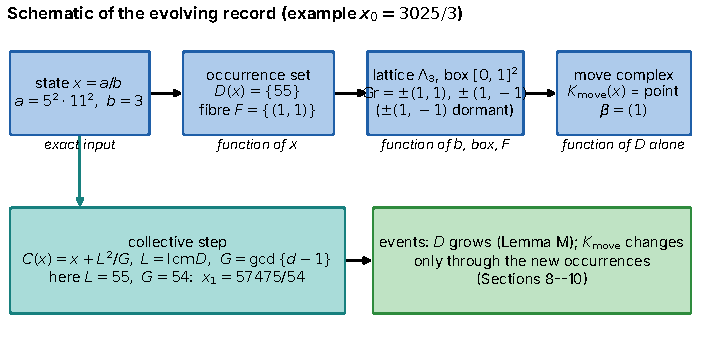
\includegraphics[width=\textwidth]{fig01_record}
\caption{\textbf{The evolving record (schematic; example values exact).} A reduced state $x=a/b$ determines its occurrence set $D(x)$ and fibre; the lattice $\Lambda_b$ and the region-Graver set depend on $b$ and the exponent box; the move complex $\Kmove$ is a function of $D$ alone (\cref{thm:R3T1a}). The collective map $C$ moves the state; the occurrence set can only grow (\cref{lem:M}); the move complex changes only through new occurrences (\cref{sec:interval}). Example $x_0=3025/3$.}\label{fig:record}
\end{figure}

\paragraph{Contributions.}
The results are organised in thirteen groups, EIII-1 to EIII-13. Each restates source records of the programme's allocation for this manuscript, which are tagged in the text by their identifiers (Appendix~\ref{app:crosswalk}).
\begin{enumerate}[leftmargin=2.7em,itemsep=2pt]
\item[\textbf{EIII-1}] \emph{Integer collapse} (\cref{sec:rational}). The complete record of an integer state is a function of its square-root content $\sigma$; the move complex is a box complex with the origin cell removed and is contractible (\cref{thm:B2T1}).
\item[\textbf{EIII-2}] \emph{Rational completeness versus relation incompleteness} (\cref{sec:rational}). For rational states the realised geometry is a function of $D(x)$ alone (\cref{thm:R3T1a}), but $D(x)$ does not determine the Graver relations: infinite families with equal $D$ and different Graver sets, for every number $k\ge2$ of primes (\cref{thm:R3T1}, uses Dirichlet's theorem), and a complete two-prime classification in seven types with one irredundant congruence bit (\cref{thm:R3T2}).
\item[\textbf{EIII-3}] \emph{Collective reduction, occurrence monotonicity, carries versus events} (\cref{sec:regimes,sec:events}). The class $G=b$ reduces to $(L,t)\mapsto(L,t+1)$ with first event at a perfect-square time (\cref{thm:R3T5a,thm:R3T5b}); $D$ is monotone along every orbit (\cref{lem:M}); arithmetic carries need not be geometric events (\cref{thm:R3T6}).
\item[\textbf{EIII-4}] \emph{Exact scaling families and a counterexample} (\cref{sec:regimes,sec:towers}). The eventual-rigidity theorem is exactly $G_\infty=1\Rightarrow$ rigid; the converse is false, with the $G=5$ tower of period $3$ and multiplier $4$ (\cref{prop:B2T7,thm:R3T5c}); the $G=11$ tower has period $8$ and multiplier $9$ (\cref{thm:R3T5bp}).
\item[\textbf{EIII-5}] \emph{The dormant-relation activation family} (\cref{sec:relations,sec:activation}). The roots $e_i-e_j$ are dormant at $x=P^2/\ell$ and realised at $y=(Pq)^2/\ell$, whose move complex is the complete graph $K_{k+1}$ with $\beta_1=\binom k2$ (\cref{thm:A4T1,thm:A4T2}).
\item[\textbf{EIII-6}] \emph{Actual dynamic activation} (\cref{sec:activation}). Reachability obstructions (a proper-divisor criterion), an eight-step orbit $3025/3\to12100/3$ with $\beta_1:0\to1$ and a $375$-step orbit with $\beta_1:0\to3$ (exact finite examples, not proofs of general reachability), and the fact that activation need not raise the Betti numbers.
\item[\textbf{EIII-7}] \emph{The exact next-event law} (\cref{sec:events}). The stage sieve $d\in D(Y_j/G)\iff Q(d)\mid Y_j$ and the resulting one-congruence-per-candidate event time; events never stop (\cref{thm:sieve,cor:event,cor:never}).
\item[\textbf{EIII-8}] \emph{Divisor-interval laws} (\cref{sec:interval}). Two occurrences are joined by an edge iff their divisor interval contains no other occurrence or $1$; when $D$ grows an old edge dies iff a new occurrence lies in its interval, and every new cell contains a new vertex (\cref{thm:A5T31,thm:A5T32}).
\item[\textbf{EIII-9}] \emph{Homology update} (\cref{sec:homology}). The zig-zag $K\leftarrow K\cap K'\to K'$ gives the identity $\Delta\beta_i=(h_i'-h_i)+(r_i'-r_i)+(r_{i-1}'-r_{i-1})$ with local $h,h'$ (\cref{thm:zigzag}) and necessary causes for any Betti change.
\item[\textbf{EIII-10}] \emph{Graph-level prediction} (\cref{sec:prediction}). Without two-cells the Betti update is predicted from the old edge set and the new occurrences alone.
\item[\textbf{EIII-11}] \emph{Event classification} (\cref{sec:prediction}). In a census of $2{,}576$ events no event is of Type~I; $1{,}787$ change the complex but no Betti number, $603$, $172$ and $14$ are of the other types (finite-exact).
\item[\textbf{EIII-12}] \emph{Nested towers} (\cref{sec:towertop}). The towers are nested filtrations without dead cells; realised moves stabilise (Graver bound $|g|_1\le\varphi(m)$); an eventual quasi-polynomial law is proved qualitatively; $G=5$ gives $(1,6,5,0)$ and $G=11$ gives $\beta_1=8$, $\beta_2=17$, $\beta_3(k+5)=\beta_3(k)+9$, all computed and verified to height $140$ and never extrapolated.
\item[\textbf{EIII-13}] \emph{Restricted correspondences and obstructions} (\cref{sec:corr}). A hierarchy of five levels of correspondence with SELECT-II, the exact classification of ratio coincidences on both towers, and the scaling obstruction: the full-period multiplier $9$ of the $G=11$ tower is not representable by any positive-length SELECT-II history.
\end{enumerate}

\paragraph{Ownership of results.}
The programme allocates to this manuscript the evolving-state, relation-lattice, occurrence-complex and collective-transformation results. A history-complex result belongs to Manuscript~II~\cite{PaperII} and a result proved in both manuscripts is proved in full in only one. Before writing, the proposed transfer was reviewed; the accepted reallocations are recorded in a derived theorem map (Appendix~\ref{app:crosswalk}) which does not alter the frozen crosswalk. In summary: the history/rewrite records B-T1--B-T9 are proved in Manuscript~II and only cited here; R3-T3, R3-T3$'$ and R3-T4 (separators and obstructions in history complexes) are cited from Manuscript~II; all other records are treated here.

\paragraph{What is not claimed.}
No physical interpretation is given. No novelty or priority claim is made. The Graver basis of the lattice is not claimed to be monotone along orbits (primitivity is not persistent; \cref{prop:A4T4b}); activation is not claimed to raise homology; tower formulas are not promoted to universal ones; finite-exact tables are never extrapolated. The programme's same-author caveat applies: all proofs and code originate from one author-collective and no independent human review is claimed. The claim C3 of the programme is not made.

\paragraph{Model boundaries.}
The collective map, the occurrence geometry and its move complexes belong to the models M5 and M8 of the programme (rational realised complexes and collective evolution). SELECT-II (M0) enters only in \cref{sec:corr}; SELECT-II is never extended to rational states. The correspondence between the integer move complex of an endpoint and the history space is cited from Manuscript~II as a non-relation (\cref{prop:A4T7}), and no map between the two dynamics is claimed (erratum ER-08).

\paragraph{Status vocabulary.}
\stat{proved} (a complete argument is given here), \stat{proved-scoped} (proved under stated hypotheses, the scope being part of the statement), \stat{finite-exact} (an exhaustive exact computation in a stated range, no claim beyond it), \stat{counterexample}, \stat{open}, \stat{cited} (taken from a released source without re-proof). \emph{Exact arithmetic} (integers and fractions, no floating point) is used in every computation; the independent engine that re-ran the finite computations of this manuscript is listed in Appendix~\ref{app:definitions}. Inherited verification suites were \emph{not re-run} (status \texttt{NOT\_RERUN}).

\paragraph{Organisation.} \Cref{sec:notation} fixes the definitions. \Cref{sec:rational,sec:relations} treat one rational state; \Cref{sec:regimes,sec:towers,sec:events} the arithmetic of the collective dynamics and of its events; \Cref{sec:activation} actual activation; \Cref{sec:interval,sec:homology,sec:prediction} the geometry of an event; \Cref{sec:towertop} the towers; \Cref{sec:corr} the correspondences; \Cref{sec:concl} the conclusions and open problems. The appendices give the source crosswalk, the definitions and engine, the complete trajectories, the relation calculations, the homology calculations and the tower tables.

\section{Collective arithmetic, occurrence geometry and notation}\label{sec:notation}
\subsection{The collective map}
\begin{definition}[collective map]\label{def:collective}
Let $x=a/b>0$ be a rational number in lowest terms. Its \emph{occurrence set} is
\[
 D(x)=\{\,d\in\Z:\ d\ge2,\ d^2\mid a,\ d\equiv1 \pmod b\,\}.
\]
The state $x$ is \emph{realised} if $D(x)\ne\emptyset$. For a realised state put
\[
 L(x)=\operatorname{lcm}D(x),\qquad G(x)=\gcd\{\,d-1:\ d\in D(x)\,\},\qquad C(x)=x+\frac{L(x)^2}{G(x)} .
\]
The map $C$ is the \emph{collective map} of the rational dynamics FIELD-I~\cite{FoundII}, in the form used by the programme (frozen releases~\cite{RefColl,HD1}). An \emph{orbit} is a sequence $x_0,x_1=C(x_0),\dots$ as long as the states are realised; $D_n=D(x_n)$, $L_n$, $G_n$ are written with the index. For an integer $x=m$ ($b=1$) the set $D(m)$ is the set of divisors $\ge2$ of the \emph{square-root content} $\sigma(m)=\prod_pp^{\lfloor v_p(m)/2\rfloor}$.
\end{definition}

\begin{lemma}[basic facts]\label{lem:basic}
Let $x=a/b$ be realised, $L=L(x)$, $G=G(x)$. Then $b\mid G$, every $d\in D(x)$ satisfies $d\equiv1\pmod G$, and $\gcd(L,G)=1$. Writing $G=bh$ one has $x=ah/G$ and $C(x)=(ah+L^2)/G$.
\end{lemma}
\begin{proof}
Every $d\in D$ is $\equiv1\pmod b$, so $b\mid d-1$ for all $d$ and $b\mid G$. Each $d-1$ is divisible by $G$ by definition of $G$, so $d\equiv1\pmod G$ and $\gcd(d,G)=1$; a prime dividing $L$ divides some $d$, hence does not divide $G$. Finally $a/b=ah/G$ and $L^2/G$ has the common denominator $G$. \qedhere
\end{proof}

\subsection{Exponent box, lattice, Graver set, move complex}
Write $a=\prod_pp^{v_p}$ and $q_p=\lfloor v_p/2\rfloor$. The \emph{active primes} are those with $q_p\ge1$; the \emph{box} is $B=\prod_{p\text{ active}}[0,q_p]\subset\Z^{k}$, $k$ the number of active primes, and for $\alpha\in B$ we write $p^\alpha=\prod p^{\alpha_p}$. Since $d^2\mid a\iff$ every exponent of $d$ is at most $q_p$, the map $\alpha\mapsto p^\alpha$ identifies the \emph{fibre} $F(x)=\{\alpha\in B\setminus\{0\}:p^\alpha\equiv1 \pmod b\}$ with $D(x)$; the origin $0\in B$ corresponds to $d=1$ and is never a vertex.

\begin{definition}[lattice, region-Graver set]\label{def:graver}
The \emph{relation lattice} of $x$ is $\Lambda_b=\{g\in\Z^k:\ \prod_pp^{g_p}\equiv1\pmod b\}$ (the primes are prime to $b$ because $a/b$ is reduced); $\Lambda_1=\Z^k$. For $g,h\in\Z^k$ write $h\sqsubseteq g$ if $h_ig_i\ge0$ and $|h_i|\le|g_i|$ for all $i$ (conformal order). The \emph{region-Graver set} $\Gr(x)$ consists of the $\sqsubseteq$-minimal non-zero elements of $\Lambda_b\cap[-q,q]$ (where $q=(q_p)$); it is a finite set closed under $g\mapsto-g$, a lattice-intrinsic object in the sense of Graver~\cite{Graver1975,Sturmfels1996}.
\end{definition}

\begin{definition}[move complexes]\label{def:Kmove}
A \emph{cell} $P(u;g_1,\dots,g_j)$ is the parallelotope $\{u+\sum_i\varepsilon_ig_i:\varepsilon\in\{0,1\}^j\}$ with $g_i\in\Gr(x)$ lexicographically positive and linearly independent; it is \emph{admissible} if all its $2^j$ vertices lie in $F(x)$. The \emph{move complex} $\Kmove(x)$ is the cubical cell complex of all admissible cells, with the usual cubical boundary $\partial P(u;g_1,\dots,g_j)=\sum_i(-1)^{i-1}\bigl(P(u+g_i;\hat g_i)-P(u;\hat g_i)\bigr)$ (see~\cite{Kozlov2008} for cubical chain complexes). The \emph{axis complex} $\Kaxis(x)$ is defined in the same way with the generators restricted to the unit vectors. Homology is taken with coefficients in a field; the Betti numbers recorded in this manuscript were computed over $\F_2$, and over $\F_p$ for $p=2^{31}-1$ in all cases where the two were compared they agree.
\end{definition}
The complexes $\Kmove$ and $\Kaxis$ are \emph{not} identified with the full realised complex of Manuscript~I nor with any history complex of Manuscript~II (\cref{prop:A4T7}).

\begin{remark}[Betti numbers as exact data]\label{rem:exact}
Every Betti number in a table or figure of this manuscript is a rank computed with exact integer arithmetic by an independent implementation (Appendix~\ref{app:definitions}); boundary maps are checked to satisfy $\partial^2=0$ in every computation. No numerical homology is used.
\end{remark}

\subsection{Monotonicity and plateaus}
\begin{lemma}[Lemma M: occurrence sets are monotone]\label{lem:M}
For every realised state $x$, $D(x)\subseteq D(C(x))$. In particular every orbit has a non-decreasing sequence $D_0\subseteq D_1\subseteq\cdots$ and every state of it is realised.
\end{lemma}
\prov{CW-0425}{A4-T3a}{PROVED}{FULL}
\begin{proof}
Let $G=bh$ as in \cref{lem:basic}, so $C(x)=(ah+L^2)/G$. For $d\in D(x)$ we have $d^2\mid a$ and $d\mid L$, so $d^2\mid ah+L^2$, and $\gcd(d,G)=1$ because $d\equiv1\pmod G$. Let $g=\gcd(ah+L^2,G)$; then $C(x)=a'/b'$ with $a'=(ah+L^2)/g$, $b'=G/g$. Since $g\mid G$ is prime to $d$, still $d^2\mid a'$; and $b'\mid G\mid d-1$ gives $d\equiv1\pmod{b'}$. Hence $d\in D(C(x))$. \qedhere
\end{proof}

\begin{definition}[events and plateaus]\label{def:event}
A step $x_n\to x_{n+1}$ is a \emph{$D$-event} if $D_n\ne D_{n+1}$; a maximal run of steps without events is a \emph{plateau} (or \emph{stage}). The sets $N=D_{n+1}\setminus D_n$ are the \emph{new occurrences}.
\end{definition}
Between events $L$ and $G$ are constant, so a plateau is an arithmetic progression $x_{n+j}=x_n+jL^2/G$; the sieve of \cref{sec:events} reads the length of the plateau from one congruence.

\section{Integer-state collapse and rational geometric structure}\label{sec:rational}
This section treats one state. For integers the geometry is determined by one integer and has no topology (\cref{thm:B2T1}); for rationals the realised geometry is determined by the occurrence set (\cref{thm:R3T1a}) but the relations are not (\cref{thm:R3T1,thm:R3T2}).

\subsection{Integer states}
\begin{theorem}[collapse and contractibility of integer states]\label{thm:B2T1}
Let $m$ be an integer with $\sigma=\sigma(m)>1$, let $q_p=\lfloor v_p(m)/2\rfloor=v_p(\sigma)$ and let $k\ge1$ be the number of primes dividing $\sigma$. Then:
\begin{enumerate}[label=(\arabic*),itemsep=1pt]
\item $\Lambda_1=\Z^k$, $\Gr(m)=\{\pm e_p\}$, $\Kmove(m)=\Kaxis(m)$, and the whole record (fibre, lattice, Graver set, cells) is a function of $\sigma$; $\sigma=\max D(m)$ recovers it.
\item $|F|=|D(m)|=\prod_p(q_p+1)-1$; the number of cells is $\prod_p(2q_p+1)-2^k$; $\chi(\Kmove(m))=1$.
\item $\Kmove(m)$ is contractible: its Betti numbers are $(1,0,\dots,0)$.
\item $\Kmove(m)\subseteq\Kmove(m')$ (as cell complexes) iff $D(m)\subseteq D(m')$ iff $q(m)\le q(m')$ coordinatewise.
\end{enumerate}
\end{theorem}
\prov{CW-0395}{B2-T1}{PROVED}{FULL}
\begin{proof}
(1) For $b=1$ every vector satisfies the congruence, so $\Lambda_1=\Z^k$ and $\Gr$ consists of the minimal non-zero vectors of $[-q,q]\cap\Z^k$. A vector with at least two non-zero coordinates dominates, in the conformal order, the unit vector of any one of them, so the minimal vectors are exactly $\pm e_p$ (which lie in the box because every $q_p\ge1$). Hence $\Kmove=\Kaxis$ is the complex of unit cubes of the box $B=\prod[0,q_p]$ none of whose vertices is the origin. The fibre is $B\setminus\{0\}$; everything is read from $q$, equivalently from $\sigma=\prod p^{q_p}=\max D(m)$.

(2) The fibre has $\prod(q_p+1)-1$ points. A cell of the box complex is a pair $(u,S)$, $u\in B$, $S\subseteq\{1..k\}$ with $u+1_S\le q$; in each coordinate there are $q_p+1$ choices if $p\notin S$ and $q_p$ if $p\in S$, in total $\prod(2q_p+1)$ cells. The origin is a vertex of exactly the cells with $u=0$, which are the $2^k$ cells $(0,S)$ (all admissible since $q_p\ge1$). Their contribution to the Euler characteristic is $\sum_S(-1)^{|S|}=0$ and the full box has $\chi=1$, so $\chi(\Kmove)=1$.

(3) Let $B$ also denote the box complex (contractible, being a cell complex structure on a box), $S=[0,1]^k$ the closed star of the origin (all cells containing the origin are faces of $[0,1]^k$) and $K=\Kmove(m)$, so that $B=K\cup S$ and $K\cap S$ is the union of the facets $\{x_i=1\}$ of $S$. All these facets contain the vertex $(1,\dots,1)$, so $K\cap S$ is a cone, hence contractible. Collapsing a contractible subcomplex is a homotopy equivalence (\cite{Hatcher2002}, Prop.~0.17): $B\simeq B/S=K/(K\cap S)\simeq K$. Thus $K$ is contractible.

(4) Cells are determined by their vertices, the vertices are the points of the fibre, and $D(m)=\{p^\alpha\}$ identifies the fibre with $D$. Hence $K(m)\subseteq K(m')$ iff $F\subseteq F'$ iff $D(m)\subseteq D(m')$. If $q\le q'$ then $B\subseteq B'$; conversely $D\subseteq D'$ contains the vertices $p^{q_p}$, giving $q\le q'$. \qedhere
\end{proof}
\begin{remark}[finite-exact check]\label{rem:B2T1check}
The closed forms of (2) and the Betti numbers of (3) were recomputed with the independent engine for the first $700$ integers $m\ge4$ with $\sigma(m)>1$: no exception (\stat{finite-exact}; Appendix~\ref{app:definitions}). The consequence recorded in the programme is that, for integers, \emph{any} geometric law is a law about $\sigma$ and $q$; the topology is trivial. Persistence of occurrence vertices implies persistence of edges and cells for integers; this fails for $b>1$ (\cref{prop:A4T4b}).
\end{remark}
\Cref{fig:integer} shows the exponent box of an integer and its closed-star decomposition .
\begin{figure}[tbp]\centering
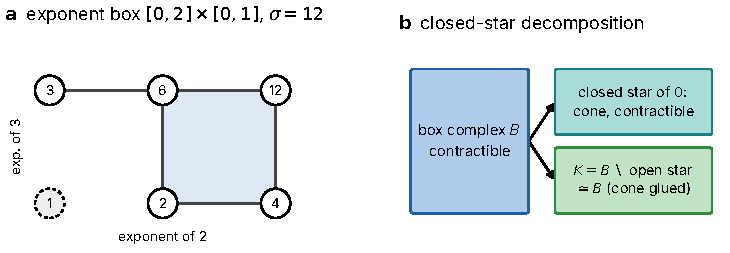
\includegraphics[width=\textwidth]{fig02_integer_collapse}
\caption{\textbf{Integer collapse (exact; proved by \cref{thm:B2T1}).} (a) The move complex of $m=2^4\,3^2\,7$, $\sigma=12$, $q=(2,1)$, drawn in exponent coordinates (a genuine grid embedding): the fibre is the box minus the origin, the shaded square is the unique cell, the dashed vertex $1$ is the removed origin. (b) The closed-star argument for contractibility.}\label{fig:integer}
\end{figure}

\subsection{Rational states: realised geometry is a function of \texorpdfstring{$D$}{D}}
\begin{lemma}[hull lemma]\label{lem:hull}
Let $x$ be a reduced rational, $u,v\in F(x)$ and $g=v-u$. Then $g\in\Gr(x)$ if and only if the coordinate hull $H(u,v)=\{w\in\Z^k:\min(u_i,v_i)\le w_i\le\max(u_i,v_i)\}$ contains no point of $F\cup\{0\}$ other than $u$ and $v$.
\end{lemma}
\begin{proof}
Since $p^u\equiv p^v\equiv1\pmod b$, $g\in\Lambda_b$, and $|g_i|\le q_i$ because $u,v\in B$. Suppose $h\in\Lambda_b$, $h\ne0,g$, $h\sqsubseteq g$. Then $w=u+h$ satisfies $w_i$ between $u_i$ and $u_i+g_i=v_i$, so $w\in H(u,v)\subseteq B$, and $p^w=p^up^h\equiv1\pmod b$, so $w\in F\cup\{0\}$ with $w\ne u,v$. Conversely a point $w\in(F\cup\{0\})\cap H(u,v)$ different from $u,v$ gives $h=w-u\in\Lambda_b$ with $h\sqsubseteq g$, $h\ne0,g$. Hence $g$ is $\sqsubseteq$-minimal in $\Lambda_b\cap[-q,q]$ iff no such $w$ exists. \qedhere
\end{proof}

\begin{theorem}[realised geometry is a function of $D$]\label{thm:R3T1a}
For a reduced rational state $x$, the fibre $F(x)$ is determined by $D(x)$, and the cell complexes $\Kaxis(x)$, $\Kmove(x)$, together with their boundary maps, components and homology, are functions of $D(x)$ alone. Moreover a pair $u,v\in F$ with $g=v-u$ is a $1$-cell of $\Kmove$ iff $H(u,v)\cap(F\cup\{0\})=\{u,v\}$, and every generator of a cell of $\Kmove$ is of this kind.
\end{theorem}
\prov{CW-0409}{R3-T1a}{PROVED}{FULL}
\begin{proof}
$F$ is recovered from $D$ by factorising $d=p^\alpha$. The cells of $\Kaxis$ are the unit cubes with all vertices in $F$. A cell $P(u;g_1,\dots,g_j)$ of $\Kmove$ has all vertices in $F$, in particular $u$ and $u+g_i$ for each $i$; by \cref{lem:hull} the condition $g_i\in\Gr(x)$ is the statement that $H(u,u+g_i)\cap(F\cup\{0\})=\{u,u+g_i\}$, a property of $F$. Linear independence and lexicographic positivity of the generators are properties of the vectors. Hence the set of cells and their boundaries are determined by $F$, and so are all derived invariants. \qedhere
\end{proof}
\begin{remark}[what lies beyond $D$]\label{rem:beyond}
\Cref{thm:R3T1a} concerns the \emph{realised} part of the record. Information beyond $D(x)$ lives in (i) \emph{dormant} Graver vectors (\cref{sec:relations}), (ii) the box and the coordinates of primes that occur in no element of $D$, and (iii) $b$ itself. For integers all of it is a function of $\sigma$ (\cref{thm:B2T1}); for rationals the realised part is not contractible in general (towers, \cref{sec:towertop}) and is generated by the congruence $d\equiv1\pmod b$.
\end{remark}

\subsection{Equal occurrence set, different relations}
\begin{theorem}[occurrence-incompleteness]\label{thm:R3T1}
\emph{(i) Two primes.} Let $r\ge13$ be a prime with $r\equiv5\pmod 8$ and put $x_r=25r^2/(5r-1)$, $y_r=25r^2/8$. Then $x_r,y_r$ are reduced, have the same active primes $\{5,r\}$, the same box $[0,1]^2$ and $D(x_r)=D(y_r)=\{5r\}$, but $\Gr(x_r)=\{\pm(1,1)\}$ and $\Gr(y_r)=\{\pm(1,1),\pm(1,-1)\}$.

\emph{(ii) $k$ primes.} Let $k\ge2$, let $\ell$ be a prime with $k\mid\ell-1$, $c\in(\Z/\ell)^*$ of exact order $k$, and $p_1,\dots,p_k$ distinct primes $\equiv c\pmod\ell$; put $P=\prod p_i$. Then $\ell\mid P-1$, and for $x=P^2/(P-1)$, $y=P^2/\ell$ one has $D(x)=D(y)=\{P\}$, box $[0,1]^k$, $\Gr(x)=\{\pm\mathbf 1\}$ and $\Gr(y)=\{\pm\mathbf 1\}\cup\{e_i-e_j:i\ne j\}$, of sizes $2$ and $k(k-1)+2$.

Both families are infinite: the primes exist, and are infinite in number, by Dirichlet's theorem on primes in arithmetic progressions~\cite{Dirichlet1837}: \emph{if $\gcd(a,m)=1$ then there are infinitely many primes $p\equiv a\pmod m$}. It is applied with $(a,m)=(5,8)$ in (i) and, in (ii), with $(a,m)=(c,\ell)$ (to choose the $p_i$) and with $(1,k)$ (to choose $\ell$).
\end{theorem}
\prov{CW-0410}{R3-T1}{PROVED}{FULL}
\begin{proof}
(i) $\gcd(25r^2,5r-1)=1$ and $\gcd(25r^2,8)=1$, so both fractions are reduced; $v_5=v_r=2$ in both numerators, so $q=(1,1)$ for the primes $(5,r)$. The fibre is contained in $\{(1,0),(0,1),(1,1)\}$. Modulo $b=5r-1$: $5\not\equiv1$ because $0<4<5r-1$; $r\not\equiv1$ because $0<r-1<5r-1$; $5r\equiv1$. Modulo $b=8$: $5\not\equiv1$, $r\equiv5\not\equiv1$, $5r\equiv25\equiv1$. So $F=\{(1,1)\}$ and $D=\{5r\}$ for both. The vector $(1,-1)$ lies in $\Lambda_b$ iff $5\equiv r\pmod b$. For $b=5r-1$ this would need $5r-1\mid r-5$, impossible since $0<|r-5|<5r-1$; for $b=8$ it holds as $r\equiv5$. The vectors $(1,0),(0,1)$ are not in $\Lambda_b$ in either case, so $\Lambda_b\cap[-1,1]^2=\{0,\pm(1,1)\}$ for $x_r$ and $\{0,\pm(1,1),\pm(1,-1)\}$ for $y_r$. The vectors $(1,1)$ and $(1,-1)$ are incomparable in the conformal order, so these sets are the Graver sets.

(ii) $P\equiv c^k\equiv1\pmod\ell$, so $\ell\mid P-1$; both fractions are reduced and the box is $[0,1]^k$. For $x$: for a non-empty $T\subseteq[k]$ put $p_T=\prod_{i\in T}p_i$. If $T\ne[k]$ then $0<p_T-1<P-1$, so $p_T\not\equiv1\pmod{P-1}$; hence $F=\{\mathbf 1\}$. A vector $1_{T_+}-1_{T_-}$ with $T_\pm$ disjoint and non-empty lies in $\Lambda_{P-1}$ iff $p_{T_+}\equiv p_{T_-}\pmod{P-1}$; both numbers lie in $[2,P/2]$ and are different (unique factorisation), so their difference is non-zero of absolute value $<P-1$: impossible. The vectors $1_T$ with $T\ne[k]$ are not in the lattice either. Hence $\Lambda\cap\{-1,0,1\}^k=\{0,\pm\mathbf 1\}$, and $\Gr(x)=\{\pm\mathbf 1\}$ (sub-vectors of $\mathbf 1$ are $1_T$). For $y$: $p_T\equiv c^{|T|}\pmod\ell$, so $F=\{\mathbf 1\}$ and $1_{T_+}-1_{T_-}\in\Lambda_\ell$ iff $k\mid|T_+|-|T_-|$. As $|T_+|+|T_-|\le k$, this means $|T_+|=|T_-|$ or $(T_+,T_-)=([k],\emptyset)$ or the reverse. A vector with $|T_+|=|T_-|\ge1$ dominates $e_i-e_j$ for $i\in T_+$, $j\in T_-$, and $e_i-e_j\in\Lambda_\ell$ is minimal (its proper sub-vectors are $\pm e_i$ or $\pm e_j$, of sum $\pm1\not\equiv0\bmod k$ since $k\ge2$); the vectors $\pm\mathbf 1$ are minimal because $1_T\notin\Lambda_\ell$ for $T\ne[k]$. These are all the minimal elements. \qedhere
\end{proof}
\begin{example}[$r=13$]\label{ex:r13}
$x_{13}=4225/64$ and $y_{13}=4225/8$ both have $D=\{65\}$; $\Gr$ has $2$ resp.\ $4$ elements (\cref{fig:equalD}). For $k=2,3,4$ the sizes $2$ versus $k(k-1)+2=4,8,14$ were recomputed by brute force with the independent engine, for $(\ell;p_i)=(3;5,11)$, $(7;23,37,79)$ and $(5;7,17,37,47)$ (\stat{finite-exact} confirmation of the proved formula).
\end{example}
\begin{figure}[tbp]\centering
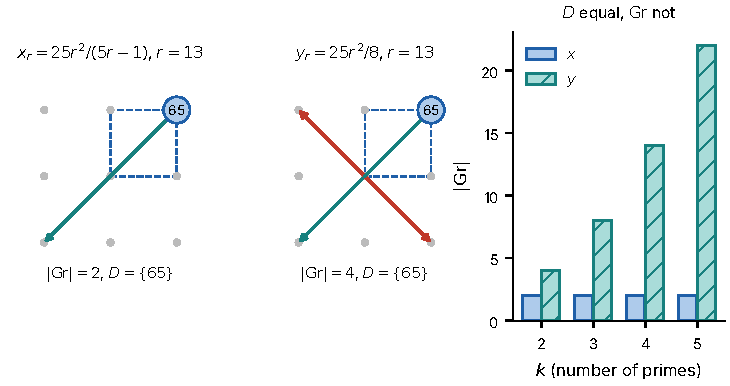
\includegraphics[width=\textwidth]{fig03_equalD_diffGr}
\caption{\textbf{Equal $D$, different Graver sets (exact; proved by \cref{thm:R3T1}).} Left, centre: the exponent plane of $(5,r)$ for $x_r$ and $y_r$, $r=13$; the dashed square is the box, the vertex is $65=5\cdot13$ at $(1,1)$ (the fibre), arrows are the Graver vectors; the red arrows $\pm(1,-1)$ are dormant. Right: sizes of the Graver sets for $x=P^2/(P-1)$ and $y=P^2/\ell$ ($k=2,3,4$ recomputed; $k=5$ is the proved formula).}\label{fig:equalD}
\end{figure}

\subsection{Two primes: the complete classification}
\begin{theorem}[two primes, box $(1,1)$]\label{thm:R3T2}
Let $p<r$ be primes and $x=(pr)^2/b$ with $\gcd(pr,b)=1$. Consider the four statements
\[
A:\ p\equiv1,\qquad B:\ r\equiv1,\qquad C:\ pr\equiv1,\qquad E:\ p\equiv r\qquad(\text{all mod }b).
\]
The lattice $\Lambda_b\cap\{-1,0,1\}^2$ contains $(1,0),(0,1),(1,1),(1,-1)$ exactly when $A,B,C,E$ hold. The set $T\subseteq\{A,B,C,E\}$ of true statements is one of seven:\ $\emptyset$, $\{A\}$, $\{B\}$, $\{C\}$, $\{E\}$, $\{C,E\}$, $\{A,B,C,E\}$; and
\[
\Gr=\emptyset,\ \pm(1,0),\ \pm(0,1),\ \pm(1,1),\ \pm(1,-1),\ \{\pm(1,1),\pm(1,-1)\},\ \{\pm(1,0),\pm(0,1)\}
\]
respectively. Moreover $D=\{p\mid A\}\cup\{r\mid B\}\cup\{pr\mid C\}$. Consequently $D$ determines the type except that $D=\emptyset$ occurs for the types $\emptyset$ and $\{E\}$ and $D=\{pr\}$ for $\{C\}$ and $\{C,E\}$; the bit $e=[E]$ is necessary and sufficient to complete $D$ to the type, i.e.\ $\Gr=\Phi(D,e)$ with $e$ irredundant.
\end{theorem}
\prov{CW-0411}{R3-T2}{PROVED}{FULL}
\begin{proof}
The four vectors are in the lattice iff the stated congruences hold. Lattice closure: $(1,0)+(0,1)=(1,1)$, $(1,0)-(0,1)=(1,-1)$, $(1,1)-(1,0)=(0,1)$, $(1,-1)+(0,1)=(1,0)$. Hence $A\wedge B$ forces $C,E$; $A\wedge C$ forces $B$ and then all; $A\wedge E$ forces $B$ (via $(1,0)-(1,-1)$) and all; $B\wedge C$ forces $A$; $B\wedge E$ forces $A$. The remaining pair $C\wedge E$ forces nothing inside the box (the sum and difference are $(2,0),(0,2)$). Therefore the true sets are exactly the seven listed. If $A$ (resp.\ $B$) holds, $\pm(1,0)$ (resp.\ $\pm(0,1)$) dominates $(1,\pm1)$, which gives the Graver sets of the types $\{A\},\{B\},\{A,B,C,E\}$; for $\{C\}$, $\{E\}$ the lattice contains only $\pm(1,1)$ resp.\ $\pm(1,-1)$; for $\{C,E\}$ the two pairs are conformally incomparable. The fibre points are the vectors of $\{(1,0),(0,1),(1,1)\}$ in the lattice, giving $D$. Necessity of $e$: both values occur for $D=\emptyset$ and $D=\{pr\}$ (\cref{ex:twoprime}); sufficiency: the table. \qedhere
\end{proof}
\begin{example}[both values of $e$ occur]\label{ex:twoprime}
$(p,r,b)=(5,13,8)$: $E$ holds ($13\equiv5$), $C$ holds, $D=\{65\}$, type $\{C,E\}$. $(p,r,b)=(5,13,64)$: only $C$, $D=\{65\}$, type $\{C\}$. For $D=\emptyset$ (neither $A,B,C$): $(p,r,b)=(3,7,4)$ gives $3\equiv7\pmod 4$, type $\{E\}$ ($\Gr=\pm(1,-1)$, no occurrence), whereas $(3,7,5)$ gives type $\emptyset$.
\end{example}
\begin{remark}[finite-exact confirmation]\label{rem:R3T2check}
For $p\in\{2,3,5,7,11,13\}$, $r\le23$ prime, $2\le b<120$, $\gcd(pr,b)=1$, the engine computed $\Gr$ by brute force for $2{,}620$ states: the type table holds for every state, and only the seven types occur, with counts $2339,27,56,108,24,32,34$ for $\emptyset,A,B,C,E,CE,ABCE$ (\cref{fig:twoprime}; \stat{finite-exact} confirmation, Appendix~\ref{app:relations}).
\end{remark}
\begin{figure}[tbp]\centering
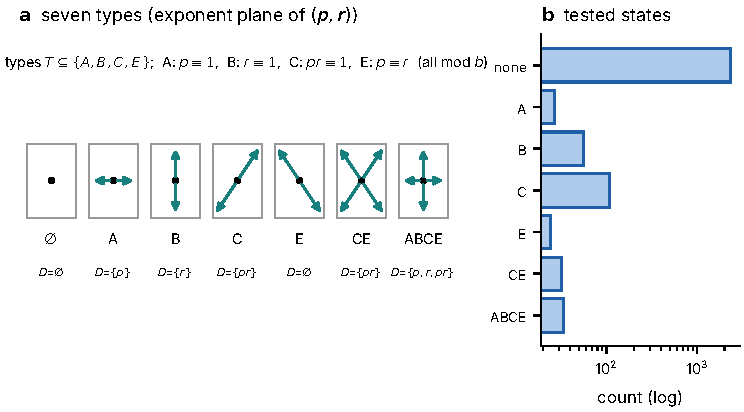
\includegraphics[width=\textwidth]{fig04_two_prime_types}
\caption{\textbf{The seven two-prime types (exact; proved by \cref{thm:R3T2}).} (a) The Graver vectors (arrows in the exponent plane of $(p,r)$) and the occurrence set of each type. (b) Number of tested states of each type among the $2{,}620$ states of \cref{rem:R3T2check} (finite-exact; log scale).}\label{fig:twoprime}
\end{figure}
\begin{problem}[R3-T2$'$: beyond two primes]\label{prob:R3T2p}
Classify the minimal descriptor $\Phi(D,J)$ beyond $D$ (the set $J$ of dormant relations) for boxes $q\ne\mathbf1^k$ and for three or more primes in full generality. Family (ii) of \cref{thm:R3T1} shows that for $q=\mathbf 1^k$ the dormant set can be the whole root system $A_{k-1}$, so the answer is a statement about lattice types, not about the number of coordinates.
\end{problem}
\prov{CW-0412}{R3-T2'}{OPEN}{OPEN}

\section{Primitive relations, dormancy and realization}\label{sec:relations}
A state carries more information than its occurrence set: the primitive relations of the region-Graver set $\Gr(x)$ include vectors that no pair of occurrences realises. This section fixes the vocabulary used for evolution and proves the exact activation family.

\subsection{Universal coordinates, active and dormant relations}
\begin{definition}[universal sparse coordinates; realisation]\label{def:universal}
Index exponent vectors by \emph{all} primes, $\Z^{(\mathbb P)}=\bigoplus_p\Z$ (finite support). A state $x_n$ of an orbit has box $B_n$ in the coordinates of its own active primes, regarded inside $\Z^{(\mathbb P)}$; $F_n\subset B_n$, $\Gr_n=\Gr(x_n)$. For $g\in\Z^{(\mathbb P)}\setminus0$ put
\[
E_g(x)=\{\,\{u,u+g\}\subset F(x)\,\}\ \ (\text{realisations of }g),\qquad g\text{ is \emph{active} at }x\iff E_g(x)\ne\emptyset .
\]
A vector $g\in\Gr(x)$ is \emph{positive} if $g\ge0$ or $g\le0$ (a pure divisibility relation), an \emph{edge relation} if it is active and not positive, and \emph{dormant} if it is not active. Since the three cases are tested in the order positive, edge, dormant, $\Gr(x)=\mathrm{Pos}\sqcup\mathrm{Edge}\sqcup\mathrm{Dormant}$. \emph{Arithmetic activation} of $g$ at step $n$ means that $g$ is active at $x_n$ and not at $x_{n-1}$; \emph{dynamical} activation concerns the change of the cell complex (\cref{sec:activation}). \emph{Creation} of $g$ means $g\in\Gr(x_n)\setminus\Gr(x_{n-1})$ (for instance because the box grew).
\end{definition}
\begin{remark}
A positive relation is an edge of the divisibility-type; in an integer state all of $\Gr=\{\pm e_p\}$ is positive and realised (\cref{thm:B2T1}). Dormancy is a phenomenon of $b>1$: the congruence conditions $d\equiv1\pmod b$ cut the fibre while $\Lambda_b$ keeps the difference vectors.
\end{remark}

\subsection{The activation family}
\begin{theorem}[activation, not creation]\label{thm:A4T1}
Let $k\ge2$, let $\ell$ be a prime with $k\mid\ell-1$, $c\in(\Z/\ell)^*$ of exact order $k$, $p_1,\dots,p_k$ distinct primes $\equiv c\pmod\ell$, $q\ne p_i$ a prime $\equiv c^{-1}\pmod\ell$, $P=\prod p_i$, and
\[
x=\frac{P^2}{\ell},\qquad y=\frac{(Pq)^2}{\ell}.
\]
Then $D(x)=\{P\}$ and $D(y)=\{P\}\cup\{p_iq:1\le i\le k\}$. For every $i\ne j$ the vector $e_i-e_j$ lies in $\Gr(x)$ and in $\Gr(y)$, is \emph{dormant at $x$} and \emph{active at $y$}: activation, not creation. Further $|\Gr(x)|=k(k-1)+2$. The move complexes of $x$ and $y$ are described in \cref{thm:A4T2}.
\end{theorem}
\prov{CW-0423}{A4-T1}{PROVED}{FULL}
\begin{proof}
\emph{Occurrence sets.} For $x$ the family is that of \cref{thm:R3T1}(ii), giving $D(x)=\{P\}$, $\Gr(x)=\{\pm\mathbf 1\}\cup\{e_i-e_j\}$, of size $k(k-1)+2$. For $y$ the active primes are $p_1..p_k,q$ and the box is $[0,1]^{k+1}$; a vertex is $p_T q^\varepsilon$ with $T\subseteq[k]$, $\varepsilon\in\{0,1\}$ not both trivial, and $p_Tq^\varepsilon\equiv c^{|T|-\varepsilon}\pmod\ell$. This is $1$ iff $|T|\equiv\varepsilon\pmod k$. For $\varepsilon=0$ only $|T|=k$ (since $T\ne\emptyset$); for $\varepsilon=1$ only $|T|=1$ (as $|T|\le k$ and $k\ge2$). Hence $D(y)=\{P,p_1q,\dots,p_kq\}$.

\emph{Edge relations.} Let $i\ne j$, $u=e_j+e_q$, $v=e_i+e_q$, so $v-u=e_i-e_j$. Both are fibre points. The coordinate hull $H(u,v)$ consists of the four points $\epsilon_ie_i+\epsilon_je_j+e_q$ ($\epsilon\in\{0,1\}^2$), and the origin is not among them; the other two, $q$ and $p_ip_jq$, have $|T|-\varepsilon=-1$ resp.\ $1$, not divisible by $k$ ($k\ge2$ for the first; for the second $k\ge2$ gives $1\not\equiv0$). By \cref{lem:hull} $e_i-e_j\in\Gr(y)$, with realisation $\{u,v\}$, so it is active. At $x$ the fibre has the single point $\mathbf 1$, so no pair of fibre points exists: $e_i-e_j$ is dormant (and it is in $\Gr(x)$ by \cref{thm:R3T1}). The same vector in both states shows that the box is the same on the primes $p_i$ and the lattice relation is the same ($d\equiv1\pmod b$ for $b=\ell$ in both), so the relation was present and is now realised.

The remaining assertions are those of \cref{thm:A4T2}. \qedhere
\end{proof}
\Cref{fig:dormant} shows the dormant and active Graver vectors at the two states.
\begin{figure}[tbp]\centering
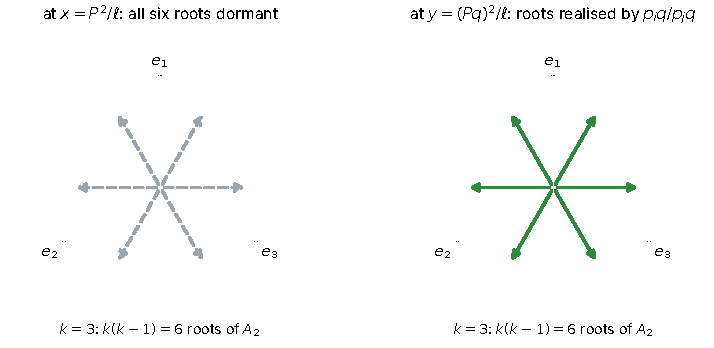
\includegraphics[width=\textwidth]{fig05_dormant_family}
\caption{\textbf{Dormant at $x$, active at $y$ (exact; proved by \cref{thm:A4T1}).} $k=2,3,4$, parameters as in the theorem. Left: $x=P^2/\ell$, a single vertex with the dormant vectors drawn as dashed arrows; right: $y=(Pq)^2/\ell$, the same vectors realised as edges of $K_{k+1}$. The move complex of $y$ is $K_{k+1}$ with no $2$-cells (\cref{thm:A4T2}), so $\beta_1=1,3,6$. The abstract objects are the relations; the geometric object is the cell complex.}\label{fig:dormant}
\end{figure}
\begin{example}[smallest member]\label{ex:A4T1}
$k=2$, $\ell=3$, $c=2$ (order $2$), $p=(5,11)$, $q=2$ ($c^{-1}=2$): $x=55^2/3$, $y=110^2/3$ with $D(y)=\{55,10,22\}$ and $\Kmove(y)$ a triangle. Further instances, $k=2$ with $q=17$ and $k=3,4,5$ with $\ell=7,5,11$, $q=11,3,3$, give $\beta_1=1,3,6,10$; they are recomputed in Appendix~\ref{app:trajectories}. The orbit of $3025/3=55^2/3$ reaches $y$-type structure (with $q=2$, not $17$) after eight steps, \cref{sec:activation}.
\end{example}

\subsection{Persistence of activity; non-persistence of primitivity}
\begin{proposition}[activity is monotone]\label{prop:A4T4a}
Along an orbit, $E_g(x_n)\subseteq E_g(x_{n+1})$ for every $g$ (in universal coordinates). Consequently $\{n:g\text{ is active at }x_n\}=[n_g,\infty)$ for an $n_g\in\N\cup\{\infty\}$.
\end{proposition}
\prov{CW-0431}{A4-T4a}{PROVED}{FULL}
\begin{proof}
In universal coordinates the fibre is the set of exponent vectors of the elements of $D(x_n)$, $F(x_n)=\{\mathrm{exp}(d):d\in D(x_n)\}$, independent of the box. A realisation $\{u,u+g\}$ is a pair of elements of $D(x_n)$, and $D(x_n)\subseteq D(x_{n+1})$ by \cref{lem:M}. \qedhere
\end{proof}
\begin{proposition}[primitivity is not persistent]\label{prop:A4T4b}
Membership $g\in\Gr(x_n)$, the $1$-cells of $\Kmove$ and $\beta_1(\Kmove)$ are not monotone along orbits. Witnesses (\stat{finite-exact}): (i) the vector $e_5-e_{11}$ lies in the lattice of the orbit of $3025/3$ at steps $n=0$ and $n=8$ only, so it is primitive-and-in-$\Gr$ at both ends and absent in between; (ii) at $57$ of the $474$ activation events of the census of \cref{sec:activation} the first Betti number of the move complex drops; (iii) for integers all geometric content is a function of $\sigma$ (\cref{thm:B2T1}), so a new occurrence can enlarge a box and destroy an edge by a divisibility relation.
\end{proposition}
\prov{CW-0432}{A4-T4b}{COUNTEREXAMPLE}{FULL}
\begin{proof}
(i) and (ii) are finite-exact computations (Appendix~\ref{app:trajectories}): along the eight-step orbit the vector $e_5-e_{11}$ is a member of $\Lambda_b\cap[-q,q]$ at $n=0$ and at $n=8$ (both with $b=3$) and of the lattice at none of the states $n=1,\dots,7$, so it is in $\Gr$ at both ends and absent in between. (iii) The orbit of $176^2/7$ at the step $5\to6$ (\cref{ex:zigzag}) has $D=\{8,22,176\}\to D'$ with nine vertices and all three old edges removed. The lattice is the same, but each old edge acquires an intermediate occurrence in its divisor interval (\cref{thm:A5T31}). \qedhere
\end{proof}

\section{Arithmetic classification of collective regimes}\label{sec:regimes}
The collective map is organised by the \emph{class number} $G(x)$. Two facts from \cref{lem:basic} drive everything: $b\mid G$, and $G(C(x))\mid G(x)$ because $D(x)\subseteq D(C(x))$ (\cref{lem:M}) and a gcd over a larger set divides the gcd over a smaller one. Hence $G_n=G(x_n)$ is eventually constant, with limit $G_\infty$, along any orbit with $D(x_0)\ne\emptyset$. We distinguish \emph{regime I} ($G=1$, integer states), \emph{class orbits} ($G=b>1$, fixed denominator) and everything else.

\subsection{Regime I: integer states with \texorpdfstring{$G=1$}{G=1}}
For an integer $m$ with $\sigma=\sigma(m)>1$ write $m=t\sigma^2$; then $t=\prod_pp^{\varepsilon_p}$ with $\varepsilon_p=v_p(m)-2q_p\in\{0,1\}$ is squarefree. Moreover $D(m)$ is the set of non-trivial divisors of $\sigma$, so $L=\sigma$.

\begin{theorem}[regime-I reduction and the rigid set]\label{thm:B2T6}
Let $m=t\sigma^2$ be as above with $G(m)=1$. Then $C(m)=(t+1)\sigma^2=t'(\sigma u)^2$ with $t'=\sqf(t+1)$ the squarefree part and $u^2=(t+1)/t'$; $G(C(m))=1$ and $\sigma(C(m))=\sigma u$. The pair $(\sigma,t)$ therefore evolves by
\[
(\sigma,t)\longmapsto(\sigma u,\ \sqf(t+1)),\qquad u=\sqrt{(t+1)/\sqf(t+1)} .
\]
The set $\{t=1,2,3\}$ is invariant, with $(\sigma,1)\to(\sigma,2)\to(\sigma,3)\to(2\sigma,1)$; on it $C^3(m)=4m$. Every orbit enters it, and the only cycle of the $t$-map $t\mapsto\sqf(t+1)$ is $(1,2,3)$.
\end{theorem}
\prov{CW-0400}{B2-T6}{PROVED}{FULL}
\begin{proof}
Since $G=1$ we have $C(m)=m+\sigma^2=(t+1)\sigma^2$. Writing $t+1=t'u^2$ gives the displayed form and $\sigma(C(m))=\sigma u$ (the $t'$ part is squarefree). By \cref{lem:basic}, $G(C(m))\mid G(m)=1$. The three steps for $t\in\{1,2,3\}$ follow from $\sqf(2)=2$, $\sqf(3)=3$, $\sqf(4)=1$ with $u=2$ at the last step; hence $C^3(\sigma^2)=4\sigma^2$, and likewise for $2\sigma^2,3\sigma^2$.

\emph{Descent.} Let $t\ge4$ be squarefree and write $t_0=t$, $t_{j+1}=\sqf(t_j+1)$. As long as $t_j+1$ is squarefree, $t_{j+1}=t_j+1$. Among $t+1,\dots,t+4$ one number is divisible by $4$, hence not squarefree; so there is a first $j\le3$ with $t+j+1$ not squarefree, and then $t_{j+1}=\sqf(t+j+1)\le(t+j+1)/4\le(t+4)/4<t$. Thus within four steps the value of $t$ drops strictly below its starting value, and by induction on $t$ every orbit reaches $t\le3$, i.e. the set $\{1,2,3\}$ of squarefree values below $4$. A cycle other than $(1,2,3)$ would contain its minimum $t_*\ge4$ and would then have to drop below $t_*$, a contradiction. \qedhere
\end{proof}
\begin{remark}[entry times; finite-exact]\label{rem:entry}
The entry time into $\{1,2,3\}$ depends only on $t$. For all squarefree $t<3000$ the maximum number of applications of $t\mapsto\sqf(t+1)$ needed is $12$ (attained at $t=1301$); the identity $C^3(m)=4m$ was also confirmed for $90$ integers of the rigid domain (\stat{finite-exact}).
\end{remark}

\subsection{Eventual rigidity: the corrected statement}
\begin{definition}[rigid]\label{def:rigid}
An orbit is \emph{rigid} if $x_{n+3}=4x_n$ for all large $n$, i.e.\ it has period $3$ with multiplier $4$ (the case of the rigid set above).
\end{definition}
\begin{proposition}[eventual rigidity; B2-T7, corrected]\label{prop:B2T7}
\begin{enumerate}[label=(\alph*),itemsep=1pt]
\item If $G_\infty=1$, the orbit is eventually an integer orbit of regime~I and is eventually rigid; the entry time after the first index with $G_n=1$ depends only on the value of $t$ at that index.
\item The converse is false: there are rigid orbits with $G_\infty=5$ (the tower of \cref{thm:R3T5c}).
\end{enumerate}
Consequently ``rigidity $\Leftrightarrow G_\infty=1$'' is not a theorem; the correct statement is \emph{only} $G_\infty=1\Rightarrow$ rigidity.
\end{proposition}
\prov{CW-0401}{B2-T7}{CORRECTED}{CORRECTED}
\begin{proof}
(a) If $G_\infty=1$ then $G_N=1$ for some $N$, hence $b_N\mid G_N=1$ and $x_N$ is an integer with $\sigma(x_N)>1$ (as $D\ne\emptyset$); \cref{thm:B2T6} applies from $N$ on. (b) is \cref{thm:R3T5c}. \qedhere
\end{proof}
\begin{remark}[provenance of the correction]
The earlier wording of this item asserted ``rigid iff $G_\infty=1$''. The $G=5$ tower of \cref{sec:towers} shows that the implication from rigidity to $G_\infty=1$ is false; the forward implication is proved above and agrees with the inherited statement (FIELD-I, Thm.~32 of~\cite{FoundII}).
\end{remark}
\Cref{fig:coords} plots the collective coordinates along an orbit.
\begin{figure}[tbp]\centering
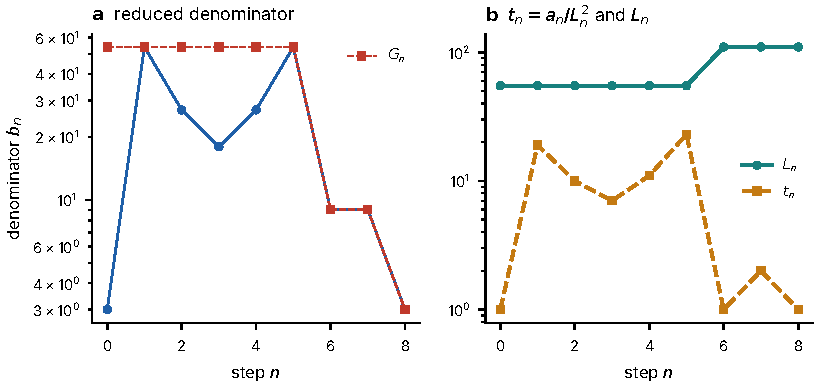
\includegraphics[width=\textwidth]{fig06_collective_coordinates}
\caption{\textbf{Collective coordinates along an orbit (exact; finite-exact data of \cref{sec:activation}).} The eight-step orbit $3025/3\to12100/3$ (parameters: $x_0=3025/3$, $n=0..8$). (a) reduced denominator $b_n$ and $G_n$ (log scale); $b_n\mid G_n$ at every step. (b) $L_n$ and $t_n=a_n/L_n^2$. Abstract quantities ($G,t$) and geometric ones ($L$) are shown together; no extrapolation.}\label{fig:coords}
\end{figure}
\begin{figure}[tbp]\centering
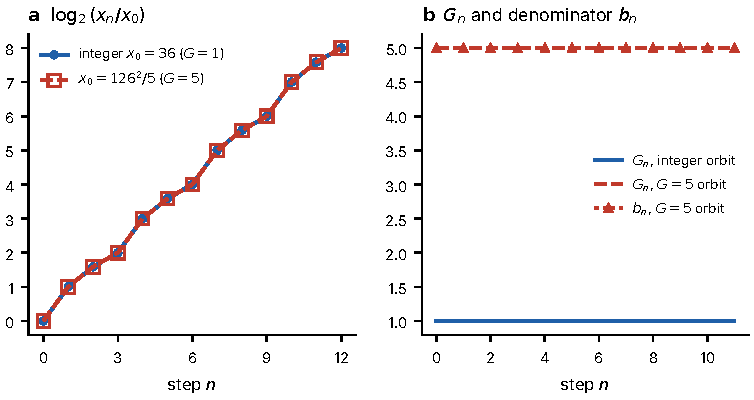
\includegraphics[width=\textwidth]{fig07_rigid_vs_persistent}
\caption{\textbf{Rigid orbits with $G=1$ and $G=5$ (finite-exact; the pattern is proved by \cref{thm:B2T6,thm:R3T5c}).} (a) $\log_2(x_n/x_0)$ for the integer orbit $x_0=36$ and for $x_0=126^2/5$, $n\le12$: both advance by $2$ every three steps, so the two curves coincide (the second is drawn with hollow markers). (b) $G_n$ for both orbits and the denominator of the second: $G$ equals $1$ resp.\ $5$ throughout, which is why rigidity does not force $G_\infty=1$.}\label{fig:rigid}
\end{figure}

\subsection{The class \texorpdfstring{$G=b$}{G=b}}
\begin{theorem}[exact reduction in the class $G(x)=b$]\label{thm:R3T5a}
Let $x=a/b$ be reduced with $D(x)\ne\emptyset$ and $G(x)=b$. Then $L^2\mid a$, so $x=tL^2/b$ with $t\in\N$, and $C(x)=(t+1)L^2/b$. If $\gcd(t+1,b)=1$ this fraction is reduced, $D(x)\subseteq D(C(x))$ and $G(C(x))=b$; if $\gcd(t+1,b)>1$ the denominator of $C(x)$ is a proper divisor of $b$ and the orbit leaves the class. While $D$ (hence $L$) is unchanged, $t$ increases by exactly $1$ per step.
\end{theorem}
\prov{CW-0416}{R3-T5a}{PROVED}{FULL}
\begin{proof}
For every prime $p$, $v_p(L)=\max_{d\in D}v_p(d)$ and $2v_p(d)\le v_p(a)$, so $L^2\mid a$. Since $G=b$ we have $h=1$ in $C(x)=(ah+L^2)/G$, giving $C(x)=(a+L^2)/b=(t+1)L^2/b$. By \cref{lem:basic}, $\gcd(L,b)=1$ (as $\gcd(L,G)=1$), so reducedness is equivalent to $\gcd(t+1,b)=1$. In that case $b\mid G(C(x))$ (basic fact for the reduced denominator $b$) and $G(C(x))\mid G(x)=b$ (monotonicity), hence equality. Otherwise cancelling the common factor shrinks the denominator. \qedhere
\end{proof}
\begin{theorem}[first event of a fresh stage; dichotomy, $b=\ell$ prime]\label{thm:R3T5b}
Let $\ell$ be prime and $x=L^2/\ell$ with $G(x)=\ell$ and $L=\lcm D(x)$ (a \emph{fresh stage}, $t=1$); write $D_\ell(S)=\{d\mid S:d\ge2,\ d\equiv1\ (\ell)\}$, so that $D(x)=D_\ell(L)$.
\begin{enumerate}[label=(\alph*),itemsep=1pt]
\item Put $u^*=\min\{u\ge2:D_\ell(uL)\ne D_\ell(L)\}$. As long as $u^{*2}<\ell$, the set $D$ is unchanged for $1\le t<u^{*2}$ and changes at $t=u^{*2}$; the stage has length $u^{*2}-1$. If $u^{*2}>\ell$ the orbit reaches the integer $L^2$ first and leaves the class.
\item Dichotomy: an orbit in the class either leaves it (becoming an integer) in finitely many steps, or has infinitely many occurrence events.
\end{enumerate}
\end{theorem}
\prov{CW-0417}{R3-T5b}{PROVED}{FULL}
\begin{proof}
(a) By \cref{thm:R3T5a} the states are $x_t=tL^2/\ell$ while $D$ is unchanged. Write $t=u_t^2\tau'$ with $\tau'$ squarefree; then $a=\tau'(u_tL)^2$ and $d^2\mid\tau'(u_tL)^2$ iff $d\mid u_tL$ (at each prime $2v_p(d)\le1+2v_p(u_tL)$ forces $v_p(d)\le v_p(u_tL)$). Hence $D(x_t)=D_\ell(u_tL)$ with $u_t^2\le t$. The sets $D_\ell(uL)$ increase with $u$ under divisibility, so for $t<u^{*2}$ we have $u_t<u^*$ and $D(x_t)=D_\ell(L)$ by minimality, while at $t=u^{*2}$, $u_t\ge u^*$ and $D$ has changed. The class is left exactly when $\ell\mid t+1$, which for $t<\ell$ first happens at $t=\ell-1$; since $\ell$ is prime $u^{*2}\ne\ell$, and $u^{*2}<\ell$ means the event comes first. (b) If there are finitely many events then $D$, hence $L$, is eventually constant, $t$ increases by one at each step (\cref{thm:R3T5a}) and $\ell\mid t+1$ within $\ell$ steps: the orbit leaves the class. \qedhere
\end{proof}
\begin{remark}
The stage that follows an event is again fresh iff $\lcm D_\ell(u^*L)=u^*L$; this holds in all the towers below, where it is verified, but it is not claimed in general (\cref{sec:towers}).
\end{remark}

\subsection{Rigid strands (finite-exact)}
\begin{proposition}[ratios along rigid strands]\label{prop:BT11}
On a rigid orbit with $x_n=t_n\sigma_n^2/b$ in the sequence $t=1,2,3,\ldots$ (the cases $G=1$ and the tower $G=5$), the consecutive ratios are $x_{n+1}/x_n=2,\ 3/2,\ 4/3$ in rotation, the displacement over one period is $4=2^2$ (exponent vector $2e_2$), and the multiplicative group generated by the ratios, $\langle2,3/2,4/3\rangle=\langle2,3\rangle$, has rank~$2$.
\end{proposition}
\prov{CW-0393}{B-T11}{FINITE-EXACT}{FINITE}
\begin{proof}
In both cases $x_n=(j+1)\sigma^2/b$ with $j=n\bmod3$ and $\sigma$ multiplied by $2$ per period: this gives the ratios $2/1,3/2,4/3$ and the product $4$. The group is generated by $2$, $3/2$, $4/3$ hence contains $3$ and $2$ and equals $\langle2,3\rangle$. \qedhere
\end{proof}
\begin{remark}
The inherited statement (FIELD-I) also records that this pattern holds on all $600$ realised states of a $20{,}000$-candidate sample; that census is \stat{cited}, not re-run. The proof above covers only the two explicit families.
\end{remark}

\section{The \texorpdfstring{$G=5$}{G=5} and \texorpdfstring{$G=11$}{G=11} towers}\label{sec:towers}
The class theorems of \cref{sec:regimes} determine an orbit once the first-event times of its stages are known. Two infinite families of fresh stages can be solved completely; they are the objects whose topology is studied in \cref{sec:towertop}. In both, ``one tower step'' replaces $S_k$ by $S_{k+1}$ and corresponds to one period of the orbit.

\subsection{The \texorpdfstring{$G=11$}{G=11} tower}
\begin{theorem}[$\ell=11$: period $8$, multiplier $9$]\label{thm:R3T5bp}
For $k\ge0$ let $S_k=2^2\,3^{3+k}\,5^4$ and $x=S_k^2/11$. Then $G(x)=11$, $L(x)=S_k$, $|D(x)|=2k+7$, and the orbit satisfies
\[
x_{8k+j}=\frac{(j+1)\,S_k^2}{11}\quad(0\le j\le8),\qquad x_{n+8}=9\,x_n,\qquad G(x_n)=11\ \text{for all }n,
\]
with exactly one occurrence event per period (at $j=8$), which creates exactly two new elements of $D$.
\end{theorem}
\prov{CW-0418}{R3-T5b'}{PROVED}{FULL}
\begin{proof}
\emph{Occurrence set.} Modulo $11$ the element $2$ is a primitive root and $3=2^8$, $5=2^4$. For $d=2^a3^c5^e$ with $a\le2$, $c\le3+k$, $e\le4$ we get $d\equiv2^{a+8c+4e}$, so $d\equiv1$ iff $a+8c+4e\equiv0\pmod{10}$. This forces $a$ even, $a\in\{0,2\}$; for $a=0$ it reads $e\equiv-2c\pmod5$, for $a=2$ it reads $e\equiv2-2c\pmod5$. For each of the $2(k+4)$ pairs $(a,c)$ there is exactly one $e\in[0,4]$. Removing $d=1$ leaves $|D|=2k+7$ (and $d\le S_k$ always has $d^2\mid S_k^2$). Since $12=2^2\cdot3\in D$ and every $d-1$ is divisible by $11$, $G=11$. The maximal exponents occur: $2^2$ in $12$; $5^4$ with $a=0,c=3$ ($e\equiv-6\equiv4$); and $3^{3+k}$ with $a=0$ and $e\equiv-2(3+k)$. Hence $L=S_k$.

\emph{One period.} By \cref{thm:R3T5a} the states while $D$ is unchanged are $x_t=tS_k^2/11$ ($t=j+1$), valid as long as $11\nmid t+1$, which holds for $t\le8$. By the proof of \cref{thm:R3T5b}, $D(x_t)=D_{11}(u_tS_k)$ with $u_t\in\{1,2\}$ for $t\le8$. The factor $2$ only raises the exponent of $2$ to $3$, which is odd and never a solution, so $D_{11}(2S_k)=D_{11}(S_k)$ and $D$ is constant for $t\le8$. At $t=9$, $u_t=3$ and the exponent of $3$ becomes $4+k$; the new solutions have $c=4+k$, one $e$ for each $a\in\{0,2\}$: exactly two new elements, and $L'=3S_k=S_{k+1}$. So $x_8=9S_k^2/11=S_{k+1}^2/11$, and the claim follows by induction on $k$ (the fresh-stage hypothesis holds at every $k$). \qedhere
\end{proof}
\Cref{fig:g11cycle} shows one period of the $G=11$ tower.
\begin{figure}[tbp]\centering
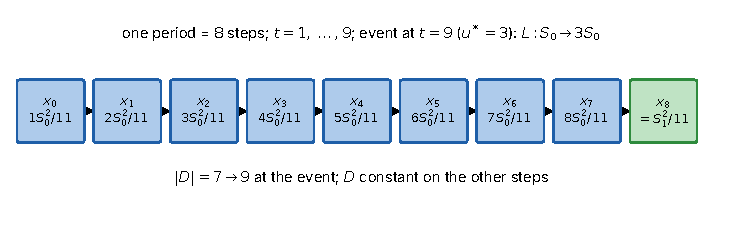
\includegraphics[width=\textwidth]{fig09_g11_cycle}
\caption{\textbf{One period of the $G=11$ tower (exact; proved by \cref{thm:R3T5bp}).} Parameters: $S_0=2^2\,3^3\,5^4$, $\ell=11$. The nine states $x_0..x_8$ of one period are drawn as boxes; $t=1,\dots,9$, the only event is at $t=9$ ($u^*=3$) where $L$ passes from $S_0$ to $3S_0$ and $|D|$ from $7$ to $9$. The orbit is abstract (arithmetic); the geometric consequence is studied in \cref{sec:towertop}.}\label{fig:g11cycle}
\end{figure}

\subsection{The \texorpdfstring{$G=5$}{G=5} tower and the failure of the converse}
\begin{theorem}[$\ell=5$: period $3$, multiplier $4$]\label{thm:R3T5c}
For $k\ge0$ let $S_k=126\cdot2^k=2^{k+1}\,3^2\,7$ and $x=S_k^2/5$. Then $G(x)=5$, $L(x)=S_k$ and
\[
x_{3k+j}=\frac{(j+1)\,S_k^2}{5}\quad(0\le j\le3),\qquad x_{n+3}=4\,x_n,\qquad G(x_n)=5\ \text{for all }n,
\]
with one event per period, at $t=4$, which creates $1$ or $2$ new elements of $D$ according as $-(k+2)\bmod4\in\{1,2\}$ or $\{0,3\}$.
\end{theorem}
\prov{CW-0419}{R3-T5c}{PROVED}{FULL}
\begin{proof}
Modulo $5$, $2$ is a primitive root, $3=2^3$ and $7\equiv2$, so $d=2^a3^c7^f\equiv2^{a+3c+f}$, which is $1$ iff $a+3c+f\equiv0\pmod4$. We have $6\in D$ ($a=1,c=1$), so $G=5$. The maximal exponents occur: for $7^1$ take $(a,c)=(0,1)$; for $3^2$ take $(a,f)=(1,1)$ ($1+6+1=8$); for $2^{k+1}$ one needs $3c+f\equiv-(k+1)\pmod4$ with $c\in\{0,1,2\}$, $f\in\{0,1\}$, and $3c+f$ takes the residues $0,1,3,0,2,3$, i.e.\ all residues. Hence $L=S_k$. The values $t=2,3$ are squarefree so $u_t=1$ and $D$ is unchanged, and $5\nmid t+1$ for $t\le3$. At $t=4$, $u_t=2$ and the exponent of $2$ rises to $k+2$; the new elements have $a=k+2$ and $3c+f\equiv-(k+2)$, which has $2,1,1,2$ solutions for the residues $0,1,2,3$ respectively. So $L'=2S_k=S_{k+1}$ and $x_3=4S_k^2/5=S_{k+1}^2/5$. \qedhere
\end{proof}
\begin{corollary}[B2-T7 is not an equivalence]\label{cor:B2T7}
The orbit of $126^2/5$ is rigid in the sense of \cref{def:rigid} with $G_\infty=5$.
\end{corollary}
\Cref{fig:g5cycle} shows one period of the $G=5$ tower.
\begin{figure}[tbp]\centering
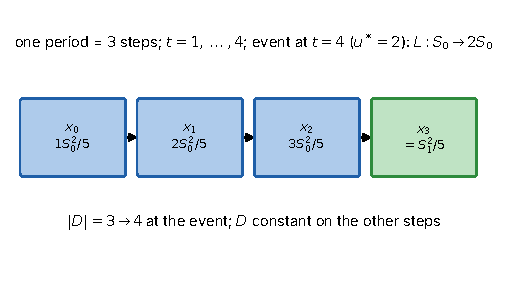
\includegraphics[width=\textwidth]{fig08_g5_cycle}
\caption{\textbf{One period of the $G=5$ tower (exact; proved by \cref{thm:R3T5c}).} Parameters: $S_0=126$, $\ell=5$. Boxes: $x_0..x_3$ with $t=1,\dots,4$; the event at $t=4$ ($u^*=2$) takes $L$ from $S_0$ to $2S_0$ and $|D|$ from $3$ to $4$. Same period and multiplier as the integer rigid orbit, but with $G=5$ rather than $1$ (\cref{fig:rigid}).}\label{fig:g5cycle}
\end{figure}

\subsection{Stage law and the \texorpdfstring{$\ell=29$}{l=29} control}
\begin{theorem}[stage law; periodic stage sequences]\label{thm:R3T5d}
Suppose an orbit in the class $G=\ell$ is a concatenation of fresh stages with first-event times $\tau_i=u_i^2$ and $L_{i+1}=u_iL_i$. Then stage $i$ lasts $\tau_i-1$ steps and multiplies $x$ by $\tau_i$. If the sequence $(\tau_i)$ is periodic with period $r$, then
\[
x_{n+P}=\rho^2x_n\ \ (n\ge n_0),\qquad P=\sum_{i<r}(\tau_i-1),\quad\rho^2=\prod_{i<r}\tau_i .
\]
The towers above are the cases $(\tau)=(9)$: $(P,\rho^2)=(8,9)$, and $(\tau)=(4)$: $(3,4)$.
\end{theorem}
\prov{CW-0420}{R3-T5d}{MIXED}{SPLIT}
\begin{proof}
At the start of stage $i$ the state is $L_i^2/\ell$; at its end, by \cref{thm:R3T5b}, it is $\tau_iL_i^2/\ell=L_{i+1}^2/\ell$. Inside a stage the state at offset $s$ is $(1+s)L_i^2/\ell$. If $\tau_{i+r}=\tau_i$ for all $i$ then $L_{i+r}=\rho L_i$ and the states of stage $i+r$ are those of stage $i$ multiplied by $\rho^2$, with the same stage lengths. \qedhere
\end{proof}
\begin{example}[$\ell=29$, $S=1890$; finite-exact]\label{ex:l29}
For $x_0=1890^2/29$ the first-event times are $\tau=(25,4,9)$ over three stages, so $P=24+3+8=35$ and $\rho^2=900$. Events occur at steps $24,27,35,59,62,70$; $x_{35}=900\,x_0$, $x_{70}=900\,x_{35}$; $G\equiv29$ throughout; the first event creates the single element $175$. This was checked with the independent engine for two full periods; \emph{periodicity for all further stages is verified, not proved}, which is why the record is split (stage law proved given periodicity; the instance finite-exact).
\end{example}
\begin{remark}[cited census]
A census of $1{,}920$ orbits $x_0=S^2/\ell$, $\ell\in\{5,\dots,29\}$ prime, of $70$--$90$ steps found among the persistent ($G>1$ forever) periodic orbits only the pairs $(P,\rho^2)=(3,4),(8,9),(35,900)$. This is \stat{cited} from the source release, not re-run, and is not a theorem.
\end{remark}

\section{Arithmetic occurrence events and their prediction}\label{sec:events}
By \cref{thm:R3T1a} the realised geometry changes only when $D$ changes. This section separates the arithmetic bookkeeping (carries, plateaus) from the occurrence events, and proves an exact sieve that predicts the next event from the current state.

\subsection{Plateaus, carries and silent carries}
\begin{proposition}[plateau theorem]\label{prop:BT10}
Let $x=a/b$ with $D(x)\ne\emptyset$ and let $\delta=L^2/G$. Along any maximal run of steps on which $D$ is unchanged, $x_{n+j}=x_n+j\delta$: a plateau is an arithmetic progression with difference $\delta=L(x)^2/G(x)$.
\end{proposition}
\prov{CW-0392}{B-T10}{MIXED}{SPLIT}
\begin{proof}
If $D$ is unchanged then $L$ and $G$ are unchanged and $C(x)=x+L^2/G$ by definition. \qedhere
\end{proof}
\begin{example}[the plateau of $1369/9$; finite-exact]\label{ex:plateau}
$x_0=37^2/9$ has $D=\{37\}$, $L=37$, $G=36$, $\delta=1369/36$. The plateau has length $140$ and ends at $x_{140}=1369\cdot144/36=5476=4\cdot37^2$, an integer with $D\ni74$ (new element $74^2=5476$).
\end{example}
\begin{remark}
The source record also asserts the ruler-function pattern of the $2$-adic valuations on a plateau and the value $\pi(c+l)$ of a rank invariant. These parts are \emph{finite-exact} in the source and are \stat{cited}, not re-derived; the record is therefore split: the arithmetic-progression statement is proved above.
\end{remark}

\begin{definition}[carry, silent carry]\label{def:carry}
A step $x_n\to x_{n+1}$ is a \emph{carry} if the box changes (in either direction), i.e.\ $q_p(x_{n+1})\ne q_p(x_n)$ for some prime $p$ (a new active prime counts as a change from $q_p=0$), and an \emph{event} if $D(x_{n+1})\ne D(x_n)$. A carry that is not an event is \emph{silent}.
\end{definition}
\begin{theorem}[occurrence changes only at carries (regime I)]\label{thm:B2T8}
On a regime-I orbit with $m_n=t_n\sigma_n^2$, $D(m_n)=\{d\mid\sigma_n:d\ge2\}$ is non-decreasing; it changes exactly at the steps with $u_n>1$ (the carries of \cref{thm:B2T6}), and at such a step the number of new elements is $\tau(\sigma_nu_n)-\tau(\sigma_n)$. In particular, for $u=2$ and $\sigma=2^a\mu$ with $\mu$ odd the count is $\tau(\mu)$.
\end{theorem}
\prov{CW-0402}{B2-T8}{PROVED}{FULL}
\begin{proof}
$D(m)=\{d\mid\sigma:d\ge2\}$, so $|D|=\tau(\sigma)-1$ and $\sigma_{n+1}=\sigma_nu_n$ by \cref{thm:B2T6}; $D$ changes iff $u_n>1$. If $u=2$ and $\sigma=2^a\mu$, then $\tau(2\sigma)-\tau(\sigma)=(a+2)\tau(\mu)-(a+1)\tau(\mu)=\tau(\mu)$. \qedhere
\end{proof}
\begin{theorem}[constancy between events; silent carries]\label{thm:R3T6}
Along any orbit the realised complexes $\Kaxis(x_n)$, $\Kmove(x_n)$ (with boundaries, components and homology) are constant on every run of steps without an event, even through carries. Silent carries occur: the box can change while $D$ is fixed (\cref{fig:carries}).
\end{theorem}
\prov{CW-0421}{R3-T6}{MIXED}{SPLIT}
\begin{proof}
Constancy is \cref{thm:R3T1a}: the realised complexes are functions of $D$. A silent carry is exhibited by the $G=11$ tower: for $x_n=(j+1)S_0^2/11$, $S_0=2^23^35^4$, the exponent $q_2(x_n)=\lfloor v_2(a_n)/2\rfloor$ follows the $2$-adic valuation of the factor $j+1$ and equals $3$ instead of $2$ at $n=3,7,11,15$ (returning at $n=4,8,12,16$), while $D$ changes only at $n=8$ and $n=16$, where $q_3$ rises (\cref{fig:carries}). \qedhere
\end{proof}
\begin{remark}
The \stat{finite-exact} part of the source record, the table of Betti vectors of the $\ell=11$ tower for $k\le11$, is superseded in this paper by the longer exact table to $k=140$ of \cref{sec:towertop}; no claim is made beyond the computed range.
\end{remark}
\begin{figure}[tbp]\centering
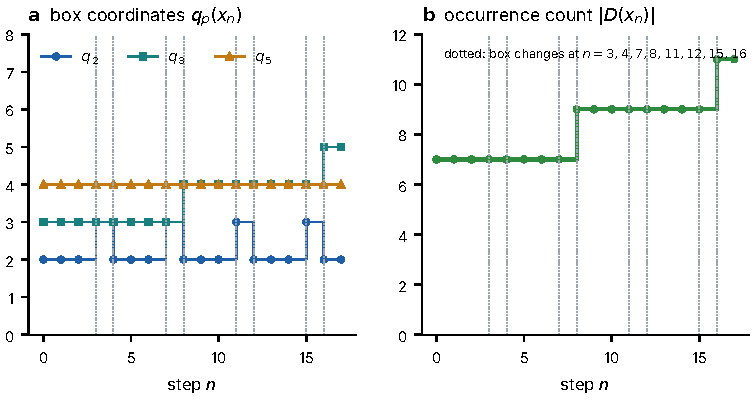
\includegraphics[width=\textwidth]{fig10_carries_vs_events}
\caption{\textbf{Carries versus events (finite-exact; illustrates \cref{thm:R3T6}).} Parameters: $G=11$ tower, $S_0=2^2\,3^3\,5^4$, $x_0=S_0^2/11$, steps $n=0..17$. (a) box coordinates $q_2,q_3,q_5$ of $x_n$ (a carry occurs wherever one of them changes; dotted lines mark the steps $n=3,4,7,8,11,12,15,16$). (b) occurrence count $|D(x_n)|$: constant except for its two jumps, at $n=8$ and $n=16$. Carries at $n=3,4,7,11,12,15$ are silent. The box coordinates are arithmetic data of the numerator; the count $|D|$ is the geometric (occurrence) datum. The range shown is the checked range.}\label{fig:carries}
\end{figure}

\subsection{The stage sieve}
Let $x=a/b$ be a state with $D(x)\ne\emptyset$, $G=G(x)=bh$, $L=L(x)$, and put $Y_j=ah+jL^2$. For a plateau starting at $x$ (so that $L,G$ are fixed), $x_{j}:=C^j(x)=Y_j/G$ as long as $D$ is unchanged; $Y_j/G$ need not be reduced.
\begin{definition}[sieve modulus]\label{def:Q}
For an integer $d\ge2$ put $r(d)=G/\gcd(d-1,G)$ and
\[
Q(d)=\lcm\Big(r(d),\ \prod_{p\mid d}p^{\,2v_p(d)+v_p(G)}\Big).
\]
\end{definition}
\begin{theorem}[stage sieve]\label{thm:sieve}
For every $j\ge0$ and every integer $d\ge2$: $d\in D(Y_j/G)\iff Q(d)\mid Y_j$.
\end{theorem}
\prov{CW-0437}{A5-T2.1}{PROVED}{FULL}
\begin{proof}
Let $g=\gcd(Y_j,G)$, $N=Y_j/g$, $B=G/g$, so $Y_j/G=N/B$ is reduced and $d\in D$ iff $d^2\mid N$ and $B\mid d-1$.

\emph{($\Rightarrow$)} Suppose $d^2\mid N$ and let $p\mid d$, $v=v_p(d)$. If $p\mid G$ then $v_p(g)=v_p(G)$: otherwise $v_p(g)=v_p(Y_j)$ and $v_p(N)=0<2v$. If $p\nmid G$, $v_p(g)=0=v_p(G)$. In both cases $v_p(Y_j)\ge2v+v_p(G)$. Next $B\mid d-1$ means $B\mid e:=\gcd(d-1,G)$, i.e.\ $G\mid eg$, i.e.\ $r(d)=G/e\mid g\mid Y_j$.

\emph{($\Leftarrow$)} If $Q(d)\mid Y_j$ then $r(d)\mid\gcd(Y_j,G)=g$, hence $B\mid d-1$ by the same equivalence. For $p\mid d$: $v_p(Y_j)\ge2v+v_p(G)$; if $p\mid G$ then $v_p(g)=v_p(G)$ and $v_p(N)=v_p(Y_j)-v_p(G)\ge2v$; if $p\nmid G$, $v_p(N)=v_p(Y_j)\ge2v$. So $d^2\mid N$. \qedhere
\end{proof}
\begin{corollary}[first-event law]\label{cor:event}
Let $\tau_D$ be the least $j\ge1$ such that some $d\notin D(x)$ satisfies $Q(d)\mid Y_j$ (equivalently $L^2j\equiv-ah\pmod{Q(d)}$). Then $D$ is unchanged for $0\le j<\tau_D$, the plateau has length $\tau_D$ and $D(x_{\tau_D})=\{d\ge2:Q(d)\mid Y_{\tau_D}\}\supsetneq D(x)$. Each candidate contributes one linear congruence, solvable iff $\gcd(L^2,Q(d))\mid ah$, with least positive solution found modulo $Q(d)/\gcd(L^2,Q(d))$.
\end{corollary}
\prov{CW-0438}{A5-T2.2}{PROVED}{FULL}
\begin{proof}
By \cref{thm:sieve}, $D(x_j)$ is the set of $d$ with $Q(d)\mid Y_j$ as long as $L,G$ are unchanged, i.e.\ until the first $j$ at which the set is larger than $D(x)$ (it always contains $D(x)$ by \cref{lem:M}). The condition $Q(d)\mid ah+jL^2$ is the stated congruence. \qedhere
\end{proof}
\begin{corollary}[events never stop]\label{cor:never}
For every state with $D\ne\emptyset$, $\tau_D<\infty$. Hence along every orbit with $D(x_0)\ne\emptyset$ there are infinitely many events and $|D(x_n)|\to\infty$.
\end{corollary}
\prov{CW-0439}{A5-T2.3}{PROVED}{FULL}
\begin{proof}
Choose a prime $p\nmid aGL$. Then $p\notin D(x)$ (since $p^2\nmid a$) and $Q(p)=r(p)p^2$ with $r(p)\mid G$ prime to $p$. The congruence $L^2j\equiv-ah\pmod{Q(p)}$ is solvable: $\gcd(L,G)=1$ (\cref{lem:basic}) and $p\nmid L$, so $L^2$ is invertible modulo $Q(p)$. Thus $\tau_D\le Q(p)<\infty$. After the event $D$ is again non-empty and strictly larger; iterate. \qedhere
\end{proof}
\Cref{fig:firstevent} illustrates the congruence for the first event.
\begin{figure}[tbp]\centering
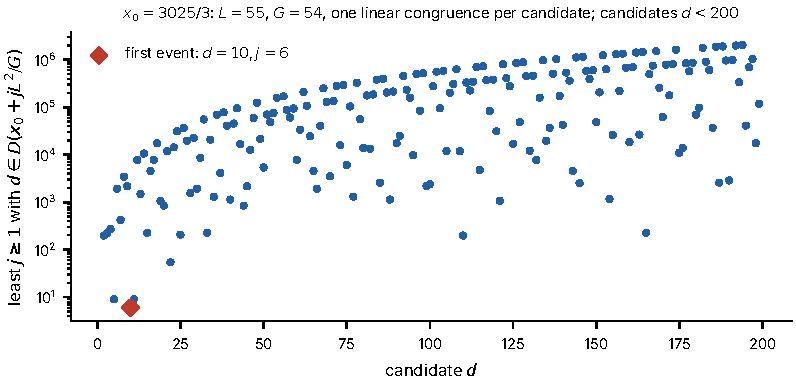
\includegraphics[width=\textwidth]{fig11_first_event}
\caption{\textbf{One linear congruence per candidate (exact computation; \cref{cor:event}).} $x_0=3025/3$: $a=3025$, $b=3$, $G=54$, $h=18$, $L=55$. Each point is a candidate $d<200$, $d\notin D$, for which the congruence is solvable, plotted at its least solution $j$. The minimum is $j=6$, attained at $d=10$ (diamond): the first event is at step $6$ and creates $10$. Finite-exact illustration, $d<200$ only; the law itself quantifies over all $d$.}\label{fig:firstevent}
\end{figure}

\subsection{Agreement with direct simulation}
\begin{remark}[finite-exact verification]\label{rem:nextevent}
The first-event law was tested against direct iteration of $C$ on $49$ states (orbits with $\tau_D\le200$ and the congruence search restricted to $\sqrt{ah+\tau L^2}\le30000$): the predicted step, and the full new set $\{d:Q(d)\mid Y_{\tau}\}$, agreed in all $49$ cases. A graph-level predictor (\cref{sec:prediction}) agreed on $175$ further events. Both are \stat{finite-exact} (\cref{fig:prediction}); no inherited suite was re-run.
\end{remark}
\begin{figure}[tbp]\centering
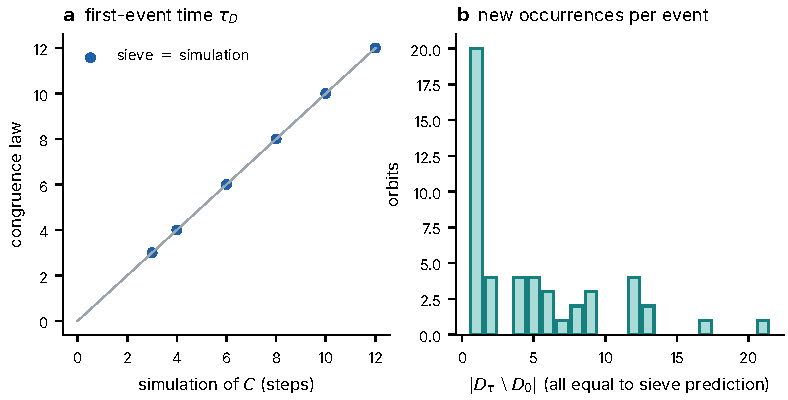
\includegraphics[width=\textwidth]{fig12_prediction}
\caption{\textbf{Prediction against reconstruction (finite-exact; $49$ states).} (a) first-event time from the congruence law versus the first event found by iterating $C$ (all points on the diagonal). (b) number of new occurrences per event; each count equals the sieve prediction. Orbits with $\tau_D\le200$ only; nothing outside this range is plotted or claimed.}\label{fig:prediction}
\end{figure}

\section{Dynamical activation}\label{sec:activation}
\Cref{thm:A4T1} exhibits a pair $(x,y)$ in which relations dormant at $x$ are realised at $y$. The dynamical question is whether $y$ lies on the collective orbit of $x$. This section proves the structure of $\Kmove(y)$, the necessary conditions, an obstruction, and a closed form for the arrival of the activating occurrences, and then presents the complete eight-step and $375$-step trajectories as exact finite examples. Throughout, the family data of \cref{thm:A4T1} are fixed; write $N=P-1=\ell m$.

\subsection{The geometry of the activated state}
\begin{theorem}[the move complex of the activated state]\label{thm:A4T2}
In the setting of \cref{thm:A4T1}, $\Kmove(y)$ is the complete graph $K_{k+1}$ on the vertices $P,p_1q,\dots,p_kq$ with no $2$-cells; hence $\beta_1(\Kmove(y))=k(k-1)/2$ and $\beta_i=0$ for $i\ge2$. $\Kaxis(y)$ is a discrete set of $k+1$ points, and $\Kmove(x)$ is a point. For $k=2$ this is a triangle with $\beta_1=1$. Moreover $|\Gr(y)|=(k+1)(k+2)$ for $k=2,\dots,5$ (\stat{finite-exact}).
\end{theorem}
\prov{CW-0424}{A4-T2}{MIXED}{SPLIT}
\begin{proof}
The fibre of $y$ is $\{P,p_1q,\dots,p_kq\}$ with exponent vectors $\mathbf 1=\sum_je_j$ and $e_i+e_q$. The vectors $e_i-e_j$ ($i\ne j$) are edges, as shown in the proof of \cref{thm:A4T1}; they join all pairs of the $k$ vertices $p_iq$. The vertex $P$ and $p_iq$ differ by $g=\sum_{j\ne i}e_j-e_q$; the coordinate hull $H(P,p_iq)$ consists of points whose $p_i$-coordinate is $1$, so it excludes the origin, and by the classification of fibre points it contains no fibre point other than the endpoints; by \cref{lem:hull}, $g\in\Gr(y)$ and $\{P,p_iq\}$ is an edge. So the $1$-skeleton is $K_{k+1}$. A $2$-cell would be a parallelogram $w_1,w_2,w_3,w_4$ of distinct fibre points with $w_1+w_4=w_2+w_3$. The $q$-coordinate is $0$ for $P$ and $1$ for each $p_iq$. If $P$ is not among the four, the relation reads $e_a+e_b=e_c+e_d$ on the $p$-coordinates with $\{a,b\}=\{c,d\}$, contradicting distinctness; if $P$ is among them, the two sides have $q$-coordinate sums $0+1$ and $1+1$ (or $0+0$ against $2$), which differ. Hence there are no $2$-cells and $\beta_1=\binom{k+1}2-k=\binom k2$ for the connected graph. $\Kaxis(y)$: two fibre points differ by a unit vector $\pm e_p$ never (their differences are of the above types), so there are no axis edges. $\Kmove(x)$ is the single fibre point $\mathbf 1$. The value $|\Gr(y)|=(k+1)(k+2)$ was found by exhaustive enumeration with the independent engine (Appendix~\ref{app:relations}). \qedhere
\end{proof}
The activation family for $k=2$ is drawn in \cref{fig:family}, and the complete graphs for larger $k$ in \cref{fig:completegraph}.
\begin{figure}[tbp]\centering
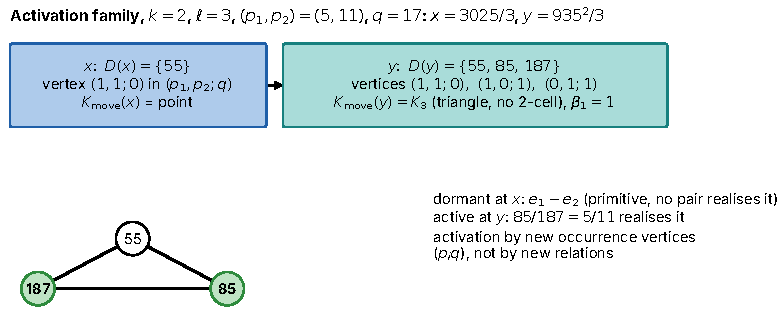
\includegraphics[width=\textwidth]{fig13_activation_family}
\caption{\textbf{The activation family, $k=2$ (exact; proved by \cref{thm:A4T1,thm:A4T2}).} Parameters: $\ell=3$, $(p_1,p_2)=(5,11)$, $q=17$, $x=3025/3$, $y=935^2/3$. Left box: $x$ has a single occurrence vertex, $55$. Right box: $y$ has $D(y)=\{55,85,187\}$ and its move complex is the triangle $K_3$ with no $2$-cell, $\beta_1=1$. The relation $e_1-e_2$ is primitive but realised by no pair at $x$ (dormant) and realised by $85/187=5/11$ at $y$: activation by new occurrence vertices, not creation of a relation. The abstract objects are the Graver vectors; the geometric object is the complex.}\label{fig:family}
\end{figure}
\begin{figure}[tbp]\centering
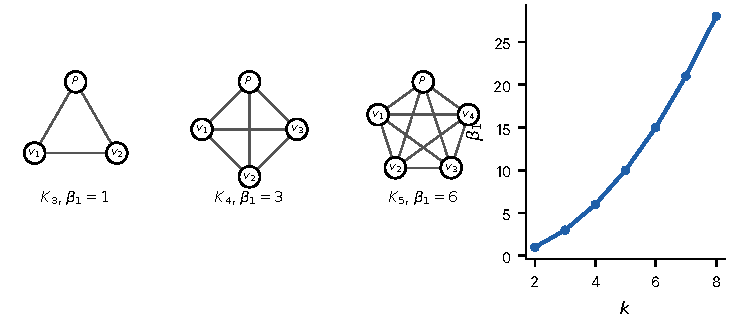
\includegraphics[width=\textwidth]{fig14_complete_graph}
\caption{\textbf{The complete graph $K_{k+1}$ (exact; proved by \cref{thm:A4T2}).} $k=2,3,4$: the move complex of $y$ with vertices $P,v_i=p_iq$ (abstract layout; not a geometric embedding), $\beta_1=1,3,6$. Right: $\beta_1=k(k-1)/2$ for $k=2,\dots,8$ is the proved formula; the values $k=2..5$ were recomputed by the engine and $k\ge6$ are formula values (labelled as such), not computations.}\label{fig:completegraph}
\end{figure}

\subsection{Progression, necessary conditions, blocking}
\begin{lemma}[progression]\label{lem:progression}
From $x=P^2/\ell$ the orbit is $x_j=P^2(m+j)/(\ell m)=P^2u/N$, $u=m+j$, as long as $D(x_j)=\{P\}$, and $P\in D(x_j)$ always. The first state with $D\ne\{P\}$ lies on this line. The line reaches $y$ exactly at $u=q^2m$.
\end{lemma}
\begin{proof}
$D(x)=\{P\}$, $L=P$, $G=P-1=N$ (as $G$ divides $N$ and $P-1\in\{d-1\}$), $b=\ell$, $h=m$, $Y_j=P^2(m+j)$. For $d=P$: $r(P)=1$ and $Q(P)=P^2$ (as $v_p(N)=0$ for $p\mid P$), so $P\in D$ by \cref{thm:sieve}. The state with $u=q^2m$ equals $P^2q^2/\ell=y$. \qedhere
\end{proof}
\begin{theorem}[necessary conditions and blocking criterion]\label{thm:A4T3b}
Suppose $y$ lies on the collective orbit of $x$. Then:
\begin{enumerate}[label=(\arabic*),itemsep=1pt]
\item every state $z$ of the orbit before $y$ satisfies $D(z)\subseteq D(y)=\{P\}\cup\{p_iq\}$;
\item at the first event, at progression index $u$, the new elements are among the $p_iq$, so $q^2\mid u/\gcd(u,N)$ and $p_iq\equiv1\pmod{b_u}$ with $b_u=N/\gcd(u,N)$;
\item the line cannot run to $u=N$: there the state is the integer $P^2$, with $p_i\in D(P^2)\setminus D(y)$.
\end{enumerate}
Conversely, \emph{any} state of an orbit with $D\not\subseteq D(y)$ blocks $y$ forever (blocking criterion).
\end{theorem}
\prov{CW-0426}{A4-T3b}{PROVED}{FULL}
\begin{proof}
(1) and the converse are \cref{lem:M}: $D$ is non-decreasing along the orbit, so a state containing an element outside $D(y)$ is followed only by such states. (2) On the line, the state $P^2u/N$ has reduced denominator $b_u=N/\gcd(u,N)$ and numerator $P^2u/\gcd(u,N)$; $d=p_iq\in D$ requires $q^2\mid u/\gcd(u,N)$ (as $q\nmid P$) and $d\equiv1\pmod{b_u}$. (3) At $u=N$ the state is $P^2\cdot N/N=P^2$; $p_i^2\mid P^2$ so $p_i\in D(P^2)$ (the denominator is $1$), whereas $p_i\notin D(y)=\{P\}\cup\{p_jq\}$ by \cref{thm:A4T1}. \qedhere
\end{proof}

\begin{theorem}[proper-divisor obstruction]\label{thm:A5T11}
For a proper divisor $1<d_0<P$, while $D=\{P\}$ one has $d_0\in D(x_u)\iff r(d_0)\mid u$, $r(d_0)=N/\gcd(d_0-1,N)$. Put $u_f=\min_{d_0}(\text{least multiple of }r(d_0)\text{ exceeding }m)$ and $u_a=\min_iu_i$ where $u_i$ is the arrival index of $p_iq$ of \cref{thm:A5T24}. If $u_f\le u_a$ and $u_f<q^2m$, then $y$ is not on the orbit of $x$ (\stat{blocked}).
\end{theorem}
\prov{CW-0453}{A5-T1.1}{PROVED}{FULL}
\begin{proof}
$P$ is squarefree and $p\mid d_0$ implies $p\nmid N$, so $Q(d_0)=\lcm(r(d_0),\prod_{p\mid d_0}p^2)$ and $Q(d_0)\mid P^2u$ iff $r(d_0)\mid u$ ($\gcd(r(d_0),P)=1$ since $r\mid N$). By \cref{thm:sieve} this is the stated equivalence. A proper divisor $d_0$ of the squarefree $P$ is not in $D(y)=\{P\}\cup\{p_iq\}$. Consider the orbit for $u<u_f$. If an event occurs at $u<u_f$, it cannot add only elements of the form $p_iq$ (those arrive at $u\ge u_a\ge u_f$), so some state has $D\not\subseteq D(y)$. If no event occurs before $u_f$, at $u=u_f$ some $d_0$ joins, with the same conclusion; and $y$ (at $u=q^2m>u_f$) was not hit meanwhile, since $D(x_u)=\{P\}\ne D(y)$ for $u<u_f$. In both cases the blocking criterion of \cref{thm:A4T3b} applies. \qedhere
\end{proof}
\begin{theorem}[arrival of the activating occurrences]\label{thm:A5T24}
While $D=\{P\}$, the occurrence $p_iq$ belongs to $D(x_u)$ iff $M_i\mid u$, where $M_i=\lcm\big(r_i,\ q^{2+v_q(N)}\big)$ and $r_i=N/\gcd(p_iq-1,N)$. The earliest arrival is at $u_i=$ the least multiple of $M_i$ exceeding $m$.
\end{theorem}
\prov{CW-0440}{A5-T2.4}{PROVED}{FULL}
\begin{proof}
Apply \cref{thm:sieve} to $d=p_iq$ with $Y=P^2u$, $G=N$: for $p=p_i$ we have $v_{p}(N)=0$ and $p^2\mid P^2$; the prime $q$ has $q\nmid P$ so $q^{2+v_q(N)}\mid P^2u$ iff $q^{2+v_q(N)}\mid u$; and $r_i\mid N$ is coprime to $P$, so $r_i\mid P^2u$ iff $r_i\mid u$. Finally $M_i\nmid m$ because $p_iq\notin D(x)$. \qedhere
\end{proof}
\begin{remark}[finite-exact check]
The closed form was compared with the sieve evaluated directly in $14$ instances: all agree (\stat{finite-exact}). The set $\{M_i\}$ is the object behind the observed phenomenon that the numerical multiplier $q^2$ is \emph{not} the mechanism of arrival: the orbit leaves the line at the first event, and arrives at $y$ by a later exact landing (examples below).
\end{remark}
\begin{counter}[``$q^2>\ell\Rightarrow$ unreachable'']\label{cx:q2l}
The initial conjecture that $q^2>\ell$ forbids reaching $y$ is false: $\ell=3$, $q=2$ has $q^2=4>3$ and $y=110^2/3$ is reached from $x=55^2/3$ in eight steps (\cref{sec:activation}, below).
\end{counter}
\prov{CW-0429}{A4-T3e}{COUNTEREXAMPLE}{EXAMPLE}

\subsection{The eight-step trajectory \texorpdfstring{$3025/3\to12100/3$}{3025/3->12100/3}}
The pair $x=55^2/3=3025/3$, $y=110^2/3=12100/3$ is the member $k=2$, $\ell=3$, $c=2$, $(p_1,p_2)=(5,11)$, $q=2$ of the family ($q=2$, not $17$). Here $P=55$, $N=54$, $m=18$.
\begin{theorem}[$x\to y$ in eight steps]\label{thm:A4T3c}
The collective orbit of $3025/3$ passes through $12100/3$ at step $8$. The denominators are $3,54,27,18,27,54,9,9,3$. The occurrence inventories, move complexes and Betti vectors are those of \cref{tab:t8}: $D=\{55\}$ for $n\le5$ (a point); one event at step $6$ ($D=\{10,55\}$, one edge, a path) and one event at step $8$ ($D=\{10,22,55\}$, a triangle with no $2$-cell). Hence $\beta_1$ passes from $0$ to $1$, at step $8$, and $y$ is reached by activation of $e_{11}-e_5$.
\end{theorem}
\prov{CW-0427}{A4-T3c}{FINITE-EXACT}{FINITE}
\begin{proof}[Exact computation]
Direct iteration of $C$ in rational arithmetic with the independent engine. The first event is predicted by \cref{cor:event,thm:A5T24}: $d=10=5\cdot2$ has $r(10)=54/\gcd(9,54)=6$, $q^{2+v_2(54)}=2^3$, $M=24$, so it arrives at $u=24$, i.e.\ at step $24-18=6$; at this step $L=110$ and $G=9$ change, and the second stage ($D=\{10,55\}$, $b=9$) lands on $y$ two steps later, with the new element $22$. \qedhere
\end{proof}
\begin{table}[tbp]\centering\small
\begin{tabular}{@{}rrrlrl@{}}\toprule
$n$ & $x_n$ & $b_n$ & $D(x_n)$ & move edges & $(\beta_0,\beta_1)$\\\midrule
0 & $3025/3$ & 3 & $\{55\}$ & 0 & $(1)$\\
1 & $57475/54$ & 54 & $\{55\}$ & 0 & $(1)$\\
2 & $30250/27$ & 27 & $\{55\}$ & 0 & $(1)$\\
3 & $21175/18$ & 18 & $\{55\}$ & 0 & $(1)$\\
4 & $33275/27$ & 27 & $\{55\}$ & 0 & $(1)$\\
5 & $69575/54$ & 54 & $\{55\}$ & 0 & $(1)$\\
6 & $12100/9$ & 9 & $\{10,55\}$ & 1 & $(1)$\\
7 & $24200/9$ & 9 & $\{10,55\}$ & 1 & $(1)$\\
8 & $12100/3$ & 3 & $\{10,22,55\}$ & 3 & $(1,1)$\\
\bottomrule\end{tabular}
\caption{\textbf{The eight-step orbit $x_0=3025/3$} (exact, \cref{thm:A4T3c}). Events occur at $n=6$ (new occurrence $10$) and $n=8$ (new occurrence $22$); the move complex of $D$ gains the edge $\{10,55\}$ at $n=6$ and the triangle with edges $\{10,22\},\{10,55\},\{22,55\}$ at $n=8$, so $\beta_1$ rises $0\to1$ at the last step only. The state $x_8=12100/3=(55\cdot2)^2/3$ is the activated target with $q=2$.}\label{tab:t8}
\end{table}

\begin{remark}[$q=2$ versus $q=17$; blocking]
For the same $x$ and $q=17$ the target $y'=935^2/3$ is blocked (\cref{thm:A5T11}: $u_f=27\le u_a=2601$ and $u_f<q^2m$; concretely the first event at step $6$ adds $10\notin D(y')$). Reachability depends on $q$, not on $q^2>\ell$ (\cref{cx:q2l}).
\end{remark}
\Cref{fig:eight} plots the eight-step trajectory of \cref{tab:t8}.
\begin{figure}[tbp]\centering
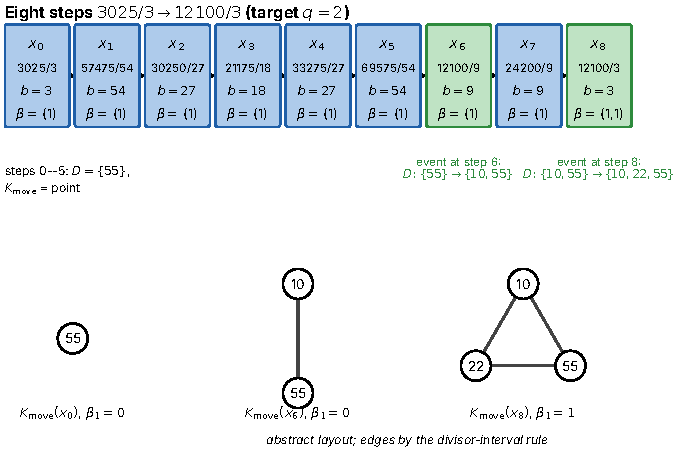
\includegraphics[width=\textwidth]{fig15_eight_step}
\caption{\textbf{The eight-step trajectory (finite-exact; exact computation).} $x_0=3025/3$, $n=0..8$, $\ell=3$, $q=2$. Each box gives $x_n$, its denominator $b_n$ and the Betti vector of $\Kmove(x_n)$ (boxes shaded green at the two event steps $6$ and $8$). Below: the move complexes at steps $0$, $6$, $8$ (abstract layout; edges by the divisor-interval rule of \cref{sec:interval}); $D$ changes only at the two events, the topology changes only at the second.}\label{fig:eight}
\end{figure}

\subsection{The \texorpdfstring{$375$}{375}-step three-prime example}
\begin{theorem}[$k=3$, $\ell=7$: $x\to y$ in $375$ steps]\label{thm:A4T3c375}
Let $(p_1,p_2,p_3)=(11,53,67)$, $P=39061$, $q=2$, $\ell=7$, $x=P^2/7$, $y=(2P)^2/7$. The orbit of $x$ reaches $y$ at step $375$. The events are at steps $372$ (new element $106=2\cdot53$), $373$ ($22=2\cdot11$) and $375$ ($134=2\cdot67$), and $\beta_1(\Kmove)$ is $0$ up to step $372$, $0$ after it, $1$ after step $373$ and $3$ after step $375$. The progression of \cref{lem:progression} alone would need $q^2m-m=16740$ steps.
\end{theorem}
\prov{CW-0427}{A4-T3c}{FINITE-EXACT}{FINITE}
This is an \emph{exact finite example}: it is computed, step by step, with the independent engine; it is not a general reachability result. The complex after the last event is $K_4$ ($P$ and the three $p_iq$, with $|D|=4$ and six edges), so $\beta_1=3$ agrees with \cref{thm:A4T2}. \Cref{fig:375} shows the denominators and the last twelve steps.
\begin{figure}[tbp]\centering
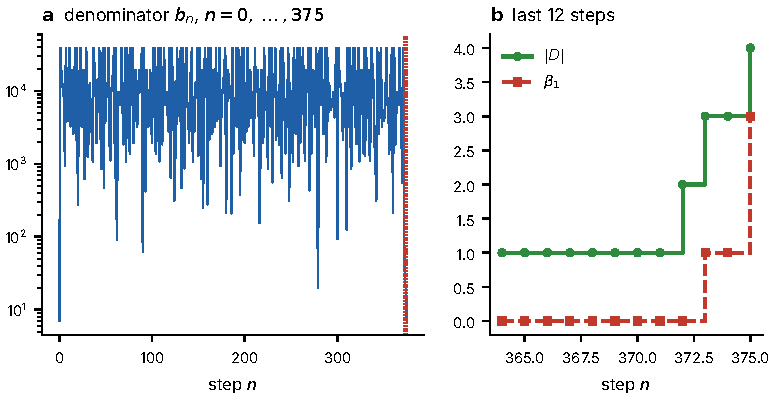
\includegraphics[width=\textwidth]{fig16_375_step}
\caption{\textbf{The $375$-step orbit (finite-exact; exact computation).} $x_0=39061^2/7$, $n=0..375$. (a) Reduced denominator $b_n$ (log scale); dotted lines mark the events at $n=372,373,375$. (b) Last twelve steps: $|D(x_n)|$ and $\beta_1$ of $\Kmove(x_n)$; $\beta_1$ is $0$ up to $n=372$, $1$ for $n=373,374$ and $3$ at $n=375$.}\label{fig:375}
\end{figure}

\subsection{Reachability scope}
The decision problem (is $y$ on the orbit of $x$?) is settled by an exact stage-jumping decider: follow the orbit stage by stage with the sieve; inside a stage landing on $y$ is an integrality condition on $(y-x_j)L^{-2}G$, and \cref{lem:M} supplies the blocking test. It is exact but not known to terminate on every input.
\begin{proposition}[cited finite data on reachability]\label{prop:reach}
The following are \stat{cited} from the source release (A4-T3c table, A5-T1.2, A5-T1.3), not re-run here:
(i) among $993$ pairs ($\ell=3$ with $q\in\{2,5,11,17,23,29\}$; $\ell=5,7$ with $k=2$; $\ell=7$, $k=3$, $q=2$), $40$ are reached, $929$ blocked, $24$ were unresolved at the step cap and none overshot; the $24$ were later decided exactly: $22$ blocked and $2$ reached (for $k=3$, $\ell=7$, $q=2$, $(67,151,179)$ in $45{,}666$ steps and $(151,179,193)$ in $67{,}756$ steps);
(ii) in a scan of $k=2$ pairs ($p<2000$, $P\le300{,}000$, $q<90$), $\ell=3$ has $52{,}997$ pairs of which $1{,}131$ are reached, $\ell=5$ has $4{,}010$ pairs of which one is reached, and the reached $q$ include $11,17$ ($\ell=3$) and $19$ ($\ell=5$: $(89,1709)$ in $2{,}239$ steps). The statement ``reached members occur only for $q\in\{2,5\}$'' is therefore false and is not repeated.
\end{proposition}
\prov{CW-0454}{A5-T1.2}{FINITE-EXACT}{CITED}
\prov{CW-0455}{A5-T1.3}{FINITE-EXACT}{CITED}
The cases re-examined here are exact: $(5,11)$, $q=2$ reached in $8$ steps; $(5,11)$, $q=17$ blocked at the first event (adds $10$); $(29,647)$, $\ell=3$, $q=11$ reached in $938$ steps; $(47,1613)$, $q=17$ in $2318$ steps; $(89,1709)$, $\ell=5$, $q=19$ in $2239$ steps; $(11,53,67)$, $\ell=7$, $q=2$ in $375$ steps (\stat{finite-exact}).
\begin{problem}[A4-T3f: infinite reached subfamily; no overshoot; closed form of the arrival step]\label{prob:A4T3f}
Is the set of reached members infinite? Is every non-blocked member reached (no overshoot; none seen among the resolved rows)? Is there a closed form for the step at which an orbit lands on $y$? \Cref{thm:A5T24} gives only the first arrival of an activating occurrence along the progression.
\end{problem}
\prov{CW-0430}{A4-T3f}{OPEN}{OPEN}

\subsection{Activation at step level, and activation without a change of Betti numbers}
\begin{proposition}[step-level activation without excursion]\label{prop:A4T3d}
(i) On the orbit of $126^2/5$ (the $G=5$ tower of \cref{thm:R3T5c}, $k=0$), at the step $5\to6$ (tower index $1\to2$) the set $D=\{6,21,36,126\}$ gains $56$, the number of dormant primitive relations drops from $6$ to $0$ and $\beta_1$ of $\Kmove$ passes from $1$ to $4$. (ii) For $\ell=29$, $x_0=1890^2/29$, at step $23\to24$ $D$ gains $175$, the number of dormant relations drops from $4$ to $2$ and the Betti vector passes from $(1)$ to $(1,1)$. (\stat{finite-exact}.)
\end{proposition}
\prov{CW-0428}{A4-T3d}{FINITE-EXACT}{FINITE}
\begin{proposition}[activation need not change Betti numbers]\label{prop:A4T4c}
There are activation events with $\beta(\Kmove)$ unchanged: the first is $\ell=5$, $S=36$, $x_0=S^2/5$, step $3\to4$, with Betti vector $(1)\to(1)$. Among the $474$ step-activation events of the source census ($\ell=5,7,11,13$; $382$ orbits), $394$ change the Betti vector, $80$ do not, and $57$ lower $\beta_1$ (\stat{cited}). In the recomputed census of all $2{,}576$ occurrence events of the orbits $x_0=S^2/\ell$ ($L=S$, $G=\ell$, $S<1500$, $24$ steps; \cref{thm:A5T7}), a different sample from the source's $474$ events,, $1{,}787$ leave the Betti vector unchanged, $603$ raise it, $172$ lower it and $14$ both raise and lower (\cref{sec:homology}). Thus the implication ``activation $\Rightarrow$ topology change'' is false in general, and it is also false that activation always raises homology.
\end{proposition}
\prov{CW-0433}{A4-T4c}{COUNTEREXAMPLE}{CITED}
\Cref{fig:unchanged} records an event with unchanged Betti numbers.
\begin{figure}[tbp]\centering
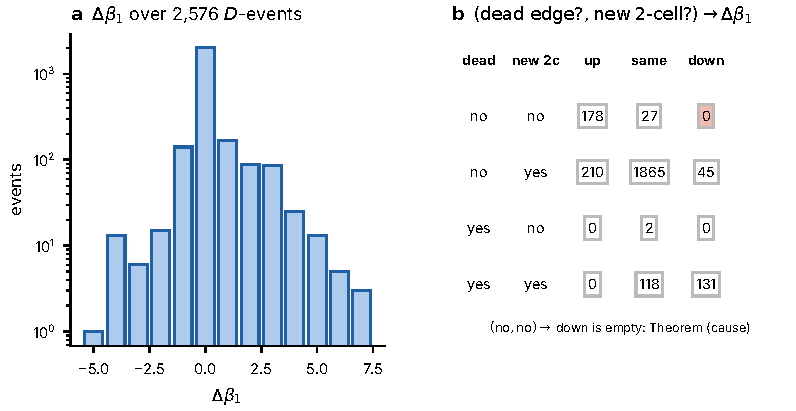
\includegraphics[width=\textwidth]{fig17_unchanged_betti}
\caption{\textbf{Occurrence events do not determine the sign of the homology change (finite-exact; $2{,}576$ events, $382$ orbits, $\ell=5,7,11,13$).} (a) Distribution of $\Delta\beta_1$ (log scale). (b) Counts by mechanism: whether the event kills an old edge (``dead'') and whether it creates a $2$-cell (``new $2$c''), against the sign of $\Delta\beta_1$. The cell (no dead edge, no new $2$-cell) with $\Delta\beta_1<0$ is empty, as proved in \cref{thm:zigzag}. Checked range only; the census is a finite sample, not a statement about all orbits.}\label{fig:unchanged}
\end{figure}

\section{Divisor-interval laws}\label{sec:interval}
Edges and cells of the move complex are decided by a local arithmetic test on divisor intervals; this turns the transition between consecutive complexes into a statement about which new occurrences fall into which old intervals.

\subsection{The edge rule}
For occurrences $u,v\in D$ write $[u,v]^\circ=\{w\in\N:\gcd(u,v)\mid w\mid\lcm(u,v)\}$ for the \emph{divisor interval}; in exponent coordinates it is the coordinate hull $H(e(u),e(v))$, with $1\leftrightarrow0$.
\begin{theorem}[divisor-interval rule]\label{thm:A5T31}
Two distinct occurrences $u,v\in D(x)$ are joined by an edge of $\Kmove(x)$ if and only if $[u,v]^\circ\cap(D\cup\{1\})=\{u,v\}$. In particular $\Kmove(x)$ is a function of $D(x)$ alone: the denominator $b$ enters only through which $D$ occurs.
\end{theorem}
\prov{CW-0441}{A5-T3.1}{PROVED}{FULL}
\begin{proof}
The $1$-cells of $\Kmove$ are the pairs $\{w,w+g\}\subseteq F$ with $g\in\Gr(x)$. By \cref{lem:hull} (with $u=e(u)$, $v=e(v)$), $v-u\in\Gr(x)$ iff the coordinate hull contains no point of $F\cup\{0\}$ other than the endpoints. Under the bijection $F\leftrightarrow D$, $0\leftrightarrow1$, the hull is $[u,v]^\circ$. \qedhere
\end{proof}
\begin{definition}[$K(D)$ for an arbitrary set]\label{def:KD}
For any finite $D\subset\N_{\ge2}$ let $K(D)$ be the cell complex with vertex set $D$, edges given by the rule of \cref{thm:A5T31}, and cells the parallelotopes $P(u;g_1,\dots,g_j)$ (lexicographically positive, linearly independent generators in the universal coordinates) all of whose $2^j$ vertices lie in $D$ and all of whose $1$-faces are edges.
\end{definition}
\begin{proposition}[intrinsic-Graver lemma]\label{prop:intrinsic}
For every state $x$, $\Kmove(x)=K(D(x))$.
\end{proposition}
\begin{proof}
A cell $P(u;g_1,\dots,g_j)$ of $\Kmove(x)$ has all vertices in $F$ and $g_i\in\Gr(x)$; its $1$-faces are the pairs $\{w,w+g_i\}\subseteq F$, which are edges by \cref{lem:hull}. Conversely if all vertices lie in $F$ and all $1$-faces are edges, then each generator $g_i=(w+g_i)-w$ with both endpoints in $F$ and $\{w,w+g_i\}$ an edge lies in $\Gr(x)$ (\cref{lem:hull}). \qedhere
\end{proof}
\begin{remark}[independent confirmation; finite-exact]
The equality was checked in the source release, with identical $f$-vectors and Betti numbers over $\F_2$ and over a large prime field, against an engine building $\Kmove$ from the lattice rather than from $D$, on $1{,}783$ states (towers, orbits for $\ell=5,7,11,13$, the activation family); that check is inherited and \stat{cited}. In the present paper the edge sets of $K(D)$ from the divisor-interval rule and from the lattice region-Graver routine were compared on $182$ states (the first $30$ steps of the orbits of $3025/3$, $126^2/5$, $1890^2/29$, $36^2/5$, $176^2/7$ and $S_0^2/11$ for $S_0=2^23^35^4$, numerators below $10^{13}$) with no mismatch (\stat{finite-exact}; script \texttt{xcheck\_KD.py}).
\end{remark}
\begin{corollary}[local consequences of the rule]\label{cor:local}
\begin{enumerate}[label=(\alph*),itemsep=1pt]
\item \emph{Coprime non-adjacency.} If $\gcd(u,v)=1$ there is no edge $\{u,v\}$, since $1\in[u,v]^\circ$.
\item \emph{Comparable pairs.} If $u\mid v$, then $\{u,v\}$ is an edge iff $u$ and $v$ are consecutive in the divisibility order of $D\cup\{1\}$.
\item \emph{Positive-primitive moves.} A positive vector $e(d)$, $d\in D$, belongs to $\Gr(x)$ iff $d$ is divisibility-minimal in $D$.
\end{enumerate}
\end{corollary}
\begin{proof}
(a) is immediate. (b) $[u,v]^\circ=\{w:u\mid w\mid v\}$. (c) The proof of \cref{lem:hull} applies with $u=0$ ($h\sqsubseteq e(d)$, $h\ne0,e(d)$, $h\in\Lambda_b$ is a point of $F$, i.e.\ a proper divisor of $d$ in $D$). \qedhere
\end{proof}

\subsection{The transition law}
Let $D\subseteq D'$ be finite sets, $N=D'\setminus D$, $K=K(D)$, $K'=K(D')$. An edge of $K$ is \emph{dead} (for $D'$) if it is not an edge of $K'$; a cell of $K$ is \emph{dead} if one of its edges is. Put $\mathrm{Dead}=\{\text{dead cells of }K\}$, $K^\circ=K\cap K'$, $\mathrm{New}=K'\setminus K$ (cells).
\begin{theorem}[transition law]\label{thm:A5T32}
\begin{enumerate}[label=(\arabic*),itemsep=1pt]
\item \emph{Non-edges persist}: a pair of $D$ that is not an edge of $K$ is not an edge of $K'$.
\item \emph{An old edge $\{u,v\}$ is dead iff some $w\in N$ lies in $[u,v]^\circ$.}
\item \emph{Every new edge and every new cell contains a new vertex.}
\item A cell dies iff one of its edges dies.
\item $K^\circ=K\setminus\mathrm{Dead}$ is a subcomplex of both $K$ and $K'$, and $K'=K^\circ\cup\mathrm{New}$.
\item \emph{Moves.} A realised move $g=e(v)-e(u)$ disappears iff every pair realising it is dead; it can appear only through a pair containing a new vertex. Consequently if $N\ne\emptyset$ is not met, no move changes: vertex growth is necessary for any change, edge loss needs a piercing new occurrence, and a new $2$-cell needs a new vertex.
\end{enumerate}
\end{theorem}
\prov{CW-0442}{A5-T3.2}{PROVED}{FULL}
\begin{proof}
(1) A non-edge $\{u,v\}$ has a point $w\in[u,v]^\circ\cap(D\cup\{1\})$, $w\ne u,v$; as $D\cup\{1\}\subseteq D'\cup\{1\}$ it is still a non-edge. (2) An old edge has no point of $D\cup\{1\}$ in its interval other than $u,v$; it is an edge of $K'$ iff there is no point of $D'\cup\{1\}$ there, i.e.\ iff no point of $N$. (3) Let $\{u,v\}$ be an edge of $K'$ with $u,v\in D$: by (1) it is an edge of $K$, so it is not new. If a cell of $K'$ has all vertices in $D$, its $1$-faces are edges of $K'$ between old vertices, hence edges of $K$, so the cell is a cell of $K$. (4) is the definition of cells of $K(D)$ via their $1$-faces. (5) The faces of a surviving cell have fewer edges, all alive, so $K\setminus\mathrm{Dead}$ is a subcomplex of $K$; a cell lies in $K'$ iff its vertices are in $D'$ and its $1$-faces are edges of $K'$, so the cells of $K$ in $K'$ are exactly the surviving ones, and the cells of $K'$ are either of $K$ (surviving) or new. (6) Disappearance and appearance of $g$ follow from (2) and (3). \qedhere
\end{proof}
\begin{corollary}[event localisation]\label{cor:localise}
At the end $\tau$ of a plateau starting at $x_0$, $N=\{d\notin D_0:Q(d)\mid Y_\tau\}$ and the dead edges are $\{\{u,v\}\in E(K(D_0)):\exists\,d\in N,\ \gcd(u,v)\mid d\mid\lcm(u,v)\}$. Both are computed from the \emph{old} complex and the congruence data of the stage; the new complex need not be built.
\end{corollary}
\prov{CW-0443}{A5-T3.3}{PROVED}{FULL}
\begin{proof}
\Cref{cor:event} gives $N$; \cref{thm:A5T32}(2) gives the dead edges. \qedhere
\end{proof}
\begin{example}[a piercing event]\label{ex:interval}
Let $D=\{8,22,176\}$, the occurrence set of $176^2/7$ at step $5$ of its orbit, and $D'=\{2,4,8,11,16,22,44,88,176\}$ at step $6$ ($N=\{2,4,11,16,44,88\}$). The three old edges are $\{8,22\}$, $\{8,176\}$, $\{22,176\}$; the intervals are $\{2,4,8,22,44,88\}$, $\{8,16,88,176\}$ and $\{22,44,88,176\}$, each of which contains a new occurrence ($2$, $16$, $44$ respectively). All three die (\cref{fig:interval}), and $K'$ has $9$ vertices, $11$ edges and $3$ squares (\cref{fig:beforeafter}).
\end{example}
\begin{figure}[tbp]\centering
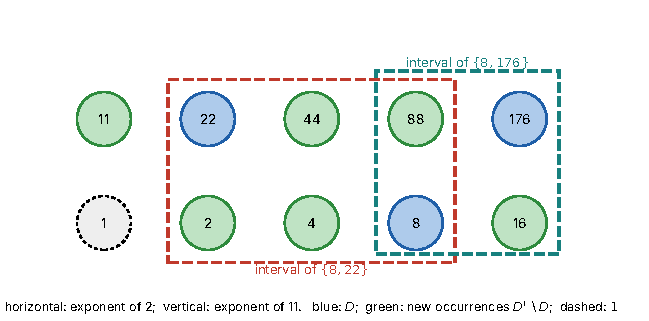
\includegraphics[width=\textwidth]{fig18_divisor_interval}
\caption{\textbf{Divisor intervals pierced by new occurrences (exact; \cref{ex:interval}, proved by \cref{thm:A5T32}).} The nine occurrences in exponent coordinates (horizontal: exponent of $2$; vertical: exponent of $11$). Blue: $D=\{8,22,176\}$ at step $5$ of the orbit of $176^2/7$; green: the new occurrences at step $6$; dashed circle: $1$. The dashed boxes are the intervals of $\{8,22\}$ and $\{8,176\}$; each contains a new occurrence. The interval of $\{22,176\}$ is pierced likewise.}\label{fig:interval}
\end{figure}
\begin{figure}[tbp]\centering
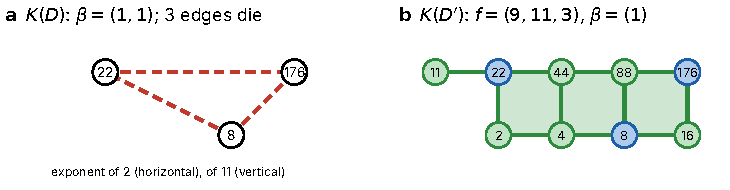
\includegraphics[width=\textwidth]{fig19_before_after}
\caption{\textbf{Before and after the same event (exact; \cref{ex:interval}).} Both complexes are drawn in exponent coordinates $(v_2,v_{11})$, a genuine planar embedding of the grid complex. (a) $K(D)$: three vertices, three dashed edges that will die, $\beta=(1,1)$. (b) $K(D')$: $9$ vertices, $11$ edges, three squares (shaded), $\beta=(1,0)$; the new edges are drawn in green. The abstract reading (which edges died) is the content of \cref{thm:A5T32}; the geometric reading is the picture.}\label{fig:beforeafter}
\end{figure}

\section{Cellular and homological transition identities}\label{sec:homology}
Let $D\subseteq D'$ be occurrence sets, $K=K(D)$, $K'=K(D')$, $K^\circ=K\cap K'=K\setminus\mathrm{Dead}$ and $\mathrm{New}=K'\setminus K$ as in \cref{thm:A5T32}. Homology is taken over a field $\mathbb k$ ($\F_2$ for all computations; the proofs hold over any field). Write $\beta_i,\beta_i'$ for the Betti numbers of $K,K'$, $\mathrm{Dead}_i,\mathrm{New}_i$ for the sets of $i$-cells, and, for the inclusions $\iota:K^\circ\to K$, $\iota':K^\circ\to K'$,
\[
\begin{aligned}r_i&=\rank(\iota_*:H_i(K^\circ)\to H_i(K)),& r_i'&=\rank(\iota'_*:H_i(K^\circ)\to H_i(K')),\\ h_i&=\dim H_i(K,K^\circ),& h_i'&=\dim H_i(K',K^\circ),\end{aligned}
\]
with the convention that all quantities of negative degree vanish. The \emph{zig-zag} $K\hookleftarrow K^\circ\hookrightarrow K'$ compares the two complexes through what survives. It is a diagram of the shape studied in zigzag persistence~\cite{CarlssonDeSilva2010} (see also~\cite{CarlssonZomorodian2009}); for this two-step case we need only the long exact sequence of a pair, and the identities below are proved directly from it.

\subsection{The zig-zag identity}
\begin{theorem}[zig-zag identity]\label{thm:zigzag}
For every $i\ge0$,
\[
\beta_i(K)=r_i+h_i-\beta_{i-1}(K^\circ)+r_{i-1},\qquad \beta_i(K')=r_i'+h_i'-\beta_{i-1}(K^\circ)+r_{i-1}',
\]
and therefore
\[
\Delta\beta_i:=\beta_i'-\beta_i=(h_i'-h_i)+(r_i'-r_i)+(r_{i-1}'-r_{i-1}).
\]
Moreover $\Delta\chi=\chi(K')-\chi(K)=\sum_i(-1)^i(|\mathrm{New}_i|-|\mathrm{Dead}_i|)$ is local: it depends only on the dead and new cells.
\end{theorem}
\prov{CW-0444}{A5-T4.1}{PROVED}{FULL}
\begin{proof}
The long exact sequence of the pair $(K,K^\circ)$ reads $\cdots\to H_i(K^\circ)\xrightarrow{\iota_*}H_i(K)\to H_i(K,K^\circ)\xrightarrow{\partial}H_{i-1}(K^\circ)\xrightarrow{\iota_*}H_{i-1}(K)\to\cdots$. By exactness, $\dim H_i(K)=\operatorname{rank}\iota_*+\operatorname{rank}(H_i(K)\to H_i(K,K^\circ))$, and the second rank equals $\dim\ker\partial=h_i-\operatorname{rank}\partial$. Again by exactness $\operatorname{rank}\partial=\dim\ker(\iota_*:H_{i-1}(K^\circ)\to H_{i-1}(K))=\beta_{i-1}(K^\circ)-r_{i-1}$. This gives the first formula; the second is the same argument for the pair $(K',K^\circ)$. Subtracting, the terms $\beta_{i-1}(K^\circ)$ cancel. For $\chi$: $K=K^\circ\sqcup\mathrm{Dead}$ and $K'=K^\circ\sqcup\mathrm{New}$ as sets of cells. \qedhere
\end{proof}
\begin{remark}[what is local]
The numbers $h_i,h_i'$ are homology of the relative chain complexes of the dead and new cells modulo $K^\circ$; $r_i,r_i'$ depend on how the surviving complex sits in $K$ and in $K'$. Everything is determined by $(D,D')$ through the rule of \cref{thm:A5T31}.
\end{remark}
\begin{example}[the piercing event of \cref{ex:interval}]\label{ex:zigzag}
$K=K(\{8,22,176\})$ is a triangle with $\beta=(1,1)$; all three edges die, so $K^\circ$ is three points, $\beta(K^\circ)=(3,0)$. Then $r=(1,0)$ (three points map onto one component) and $h=(0,3)$ (three relative $1$-cells). $K'$ has $f=(9,11,3)$ and $\beta'=(1,0)$, with $r'=(1,0)$ and $h'=(0,2)$. The identity gives $\Delta\beta_1=(2-3)+(0-0)+(1-1)=-1$ and $\Delta\beta_0=0$, as observed (\cref{fig:zigzag}). The Euler characteristic is local: $|\mathrm{Dead}|=(0,3,0)$, $|\mathrm{New}|=(6,11,3)$, so $\Delta\chi=(6-0)-(11-3)+(3-0)=1=\chi(K')-\chi(K)=1-0$. Chain-level boundary matrices and the check $\partial^2=0$ are in Appendix~\ref{app:homology}.
\end{example}
\begin{figure}[tbp]\centering
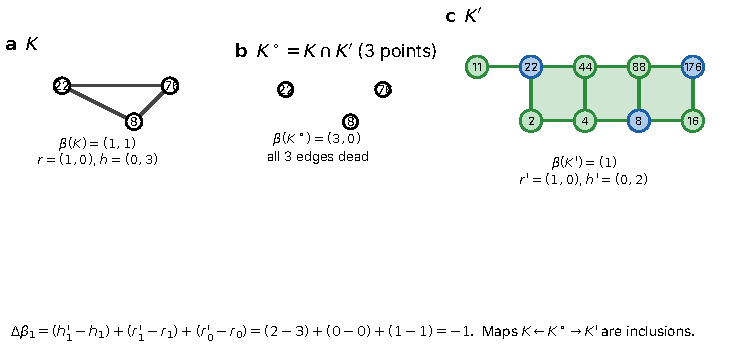
\includegraphics[width=\textwidth]{fig20_zigzag}
\caption{\textbf{The zig-zag $K\hookleftarrow K^\circ\hookrightarrow K'$ for the event of \cref{ex:interval} (exact; \cref{thm:zigzag}).} Left: $K(\{8,22,176\})$, a triangle, $\beta=(1,1)$. Centre: $K^\circ=K\cap K'$, the three surviving vertices (all three edges are dead), $\beta=(3,0)$. Right: $K(D')$, $f=(9,11,3)$, $\beta=(1,0)$. The numbers $r,h,r',h'$ of the identity are listed under the panels. The drawing is schematic (abstract layout of the complexes); the embedded version is \cref{fig:beforeafter}.}\label{fig:zigzag}
\end{figure}

\subsection{Which cells cause a change}
\begin{theorem}[cause criteria]\label{thm:cause}
For every $i\ge0$:
\begin{enumerate}[label=(\roman*),itemsep=1pt]
\item if $\Delta\beta_i<0$ then $\mathrm{Dead}_i\ne\emptyset$ or $\mathrm{New}_{i+1}\ne\emptyset$ (a cell of dimension $i$ died or a cell of dimension $i+1$ appeared);
\item if $\Delta\beta_i>0$ then $\mathrm{New}_i\ne\emptyset$ or $\mathrm{Dead}_{i+1}\ne\emptyset$.
\end{enumerate}
In particular, if no cell dies, $\Delta\beta_i<0$ forces a new $(i+1)$-cell.
\end{theorem}
\prov{CW-0445}{A5-T4.2}{PROVED}{FULL}
\begin{proof}
(i) Suppose $\mathrm{Dead}_i=\emptyset=\mathrm{New}_{i+1}$. Then $C_i(K)=C_i(K^\circ)\subseteq C_i(K')$, so $Z_i(K)\subseteq Z_i(K')$ (boundaries of cells of $K^\circ$ are computed in $K^\circ$), and $C_{i+1}(K')=C_{i+1}(K^\circ)\subseteq C_{i+1}(K)$, so $B_i(K')\subseteq B_i(K)$. Hence $\beta_i'=\dim Z_i(K')-\dim B_i(K')\ge\dim Z_i(K)-\dim B_i(K)=\beta_i$, i.e.\ $\Delta\beta_i\ge0$. (ii) Symmetrically, if $\mathrm{New}_i=\emptyset=\mathrm{Dead}_{i+1}$ then $C_i(K')\subseteq C_i(K)$, $C_{i+1}(K)\subseteq C_{i+1}(K')$, so $Z_i(K')\subseteq Z_i(K)$ and $B_i(K)\subseteq B_i(K')$ and $\beta_i'\le\beta_i$. \qedhere
\end{proof}
\begin{remark}[correction of the inherited proof]
The inherited argument for the first part used the equality $B_i(K')=B_i(K)$ when no $(i+1)$-cell is added; that is false when cells die at level $i+1$. The inclusions $Z_i(K)\subseteq Z_i(K')$ and $B_i(K')\subseteq B_i(K)$ used above are what the argument needs, and the statement is unchanged.
\end{remark}
\begin{theorem}[nested events]\label{thm:nested}
If $\mathrm{Dead}=\emptyset$ (so $K\subseteq K'$), then with $k_i=\dim\ker(H_i(K)\to H_i(K'))$ one has
\[
\Delta\beta_i=h_i(K',K)-k_i-k_{i-1}.
\]
\end{theorem}
\prov{CW-0446}{A5-T4.3}{PROVED}{FULL}
\begin{proof}
Here $K^\circ=K$, hence $h=0$, $r_i=\beta_i$ and $r_i'=\beta_i-k_i$. Substitute in \cref{thm:zigzag}. \qedhere
\end{proof}
\begin{remark}[scope]
The nested case occurs along the towers of \cref{sec:towertop} (where $\mathrm{Dead}=\emptyset$ at every tower step), but not in general along orbits: an occurrence event with $\mathrm{Dead}\ne\emptyset$ is a genuine zig-zag (\cref{ex:zigzag}).
\end{remark}

\section{Predictive graph topology and event classification}\label{sec:prediction}
\Cref{thm:zigzag} separates the change of Betti numbers into local terms and the global ranks $r,r'$. In the case where all complexes involved are graphs, the global term is one number, the change of the number of components, and the update can be carried out from the old edge set and the new occurrences.

\subsection{An exact graph-level predictor}
\begin{theorem}[graph-level update]\label{thm:A5T44}
Let $D\subseteq D'$, $N=D'\setminus D$, and suppose neither $K=K(D)$ nor $K'=K(D')$ has a $2$-cell. Let $\mathrm{Pierced}$ be the set of edges $\{u,v\}$ of $K$ with some $w\in N$ in $[u,v]^\circ$, and $\mathrm{NewEdges}$ the set of pairs $\{u,w\}$, $w\in N$, $u\in D'$, whose interval meets $D'\cup\{1\}$ only in $u,w$. Then $E(K')=(E(K)\setminus\mathrm{Pierced})\cup\mathrm{NewEdges}$ and
\[
\Delta\beta_1=\Delta E-\Delta V+\Delta\beta_0,\qquad\Delta V=|N|,\quad\Delta E=|\mathrm{NewEdges}|-|\mathrm{Pierced}|,
\]
where $\beta_0(K')$ is the number of connected components of the graph $(D',E(K'))$.
\end{theorem}
\prov{CW-0447}{A5-T4.4}{PROVED}{FULL}
\begin{proof}
The edge set of $K'$ is given by \cref{thm:A5T32}(2),(3): old edges survive unless pierced, and every other edge contains a new vertex and is detected by the interval rule against $D'\cup\{1\}$. For a graph, $\chi=V-E=\beta_0-\beta_1$, so $\beta_1=E-V+\beta_0$ for $K$ and for $K'$; subtract. \qedhere
\end{proof}
\begin{remark}[what is, and is not, claimed; control]
The predictor does not recompute old--old pairs, builds no cells and does no linear algebra: it needs the old edge set, the intervals pierced by $N$, the pairs through new vertices, and a union--find. The hypothesis that $K'$ has no $2$-cell is checked by testing parallelograms through the new vertices; it is \emph{not} dropped. For complexes with $2$-cells only the local terms and the cause criteria are arithmetic, and no rebuild-free Betti prediction in higher dimension is claimed. \emph{Control:} the activation family, $D=\{P\}\to D(y)$, $N=\{p_iq\}$, $\mathrm{Pierced}=\emptyset$, $|\mathrm{NewEdges}|=\binom{k+1}{2}$, $\Delta V=k$, $\Delta\beta_0=0$, gives $\Delta\beta_1=\binom{k+1}2-k=k(k-1)/2$, the value of \cref{thm:A4T2} obtained from the transition law alone.
\end{remark}
\begin{remark}[finite-exact test]
On the $175$ events of the census below in which neither complex has cells of dimension $\ge2$, the predicted $\beta_1(K')$ agreed with the rebuilt value in $175$ of $175$ cases (\cref{fig:graphupdate}; \stat{finite-exact}).
\end{remark}
\begin{figure}[tbp]\centering
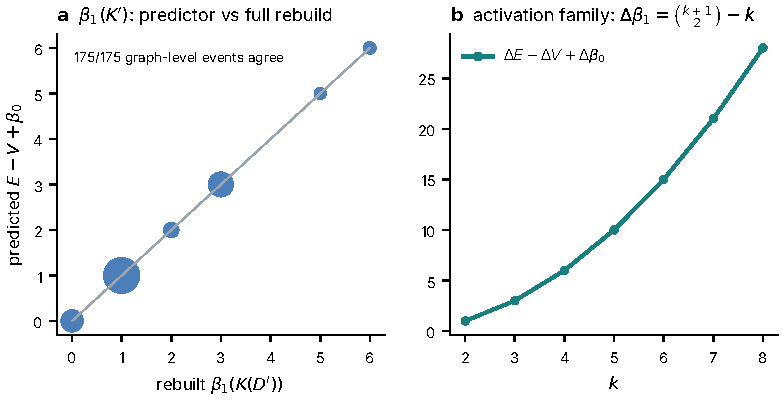
\includegraphics[width=\textwidth]{fig21_graph_update}
\caption{\textbf{Graph-level prediction (exact theorem; finite-exact test on $175$ events).} (a) Predicted $\beta_1(K')=E-V+\beta_0$ versus $\beta_1$ of the rebuilt complex, for the $175$ census events in which neither complex has $2$-cells (point size grows with multiplicity; all points lie on the diagonal). (b) $\Delta\beta_1=\binom{k+1}2-k$ for the activation family: the values for $k=2,\dots,5$ were recomputed, the points for $k=6,7,8$ are values of the proved formula, not computations.}\label{fig:graphupdate}
\end{figure}
\begin{counter}[a pierced edge with an increase of $\beta_1$ in the abstract calculus]\label{cx:abstract}
Take (as abstract sets) $D=\{56,21,32,45\}$ and $N=\{51,15,11\}$. Then $K(D)$ has edges $\{21,45\},\{21,56\},\{32,56\}$, $\beta=(1,0)$; $K(D\cup N)$ has $7$ vertices, $6$ edges, no $2$-cells and $\beta=(2,1)$; the edge $\{21,45\}$ is pierced (by $15\in[3,315]^\circ$) and $\beta_1$ nevertheless increases. This is a computation with the rule of \cref{thm:A5T31} and does not assert that such an event occurs along a collective orbit.
\end{counter}
\begin{remark}[a census regularity, not a theorem]
In the census below, the $251$ events with a dead edge never raise $\beta_1$. This regularity is not a law of the transition calculus (\cref{cx:abstract}); whether it can fail along a collective orbit is open.
\end{remark}

\subsection{Event types}
Every occurrence event adds at least one vertex. Classify an event $D\to D'$ by its effect on $(K,\beta)$:
\begin{center}\small
\begin{tabular}{@{}cl@{}}\toprule
Type & definition\\\midrule
I & the complex does not change\\
II & some $\beta_i$ increases and none decreases\\
III & some $\beta_i$ decreases and none increases\\
IV & some $\beta_i$ increases and some decreases\\
V & the Betti vector is unchanged while the complex changes\\\bottomrule
\end{tabular}
\end{center}
\begin{theorem}[no event of Type I; census]\label{thm:A5T7}
(a) Type I never occurs among occurrence events: $D\subsetneq D'$ adds a vertex, so $K\ne K'$. Hence every activation without a change of Betti numbers is of Type V.
(b) \emph{Census} (finite-exact, recomputed): for the orbits $x_0=S^2/\ell$ with $L(x_0)=S$, $G(x_0)=\ell$, $\ell\in\{5,7,11,13\}$, $S<1500$, followed for $24$ steps ($382$ orbits), the $2{,}576$ occurrence events are of Type V in $1{,}787$ cases, II in $603$, III in $172$, IV in $14$ and I in none. $251$ events have a dead edge (at most $16$ in one event) and $2{,}325$ are nested ($\mathrm{Dead}=\emptyset$); $\beta_2$ changes in $246$ events and $\beta_3$ in one; $\beta_1$ decreases in $176$ and increases in $388$. In each event the structural statements of \cref{thm:A5T32}, the zig-zag identity, the reconstruction of $\beta(K)$ and $\beta(K')$ from $(r,h,\beta(K^\circ))$, the local Euler formula and the cause criteria of \cref{thm:cause} hold (no exception).
(c) Table of the dependence of $\Delta\beta_1$ on the cause, ``dead edge?'' and ``new $2$-cell?'': (no,no): $178$ up, $27$ same, $0$ down; (no,yes): $210$, $1865$, $45$; (yes,no): $0$, $2$, $0$; (yes,yes): $0$, $118$, $131$. The empty ``down'' entry of (no,no) is \cref{thm:cause}; the zeros in the ``up'' column of both dead-edge rows are a census regularity (see above).
\end{theorem}
\prov{CW-0452}{A5-T7}{MIXED}{SPLIT}
\begin{proof}
(a) is the definition. (b), (c) are computations with the engine of Appendix~\ref{app:definitions}; the proved parts are those named. \qedhere
\end{proof}
\begin{remark}[no predictive predicate for the type]
What is proved is the \emph{form} of the answer: the type is determined by $(K(D),N)$, and $N$ is arithmetic (\cref{cor:event}). No arithmetic predicate of the state alone is claimed to predict the type; that is an open problem (\cref{sec:concl}). The inherited cross-check, that all $474$ step-activation events of the source census have the same Betti vectors before and after under this engine, is \stat{cited}.
\end{remark}
The distribution of event types is shown in \cref{fig:types}.
\begin{figure}[tbp]\centering
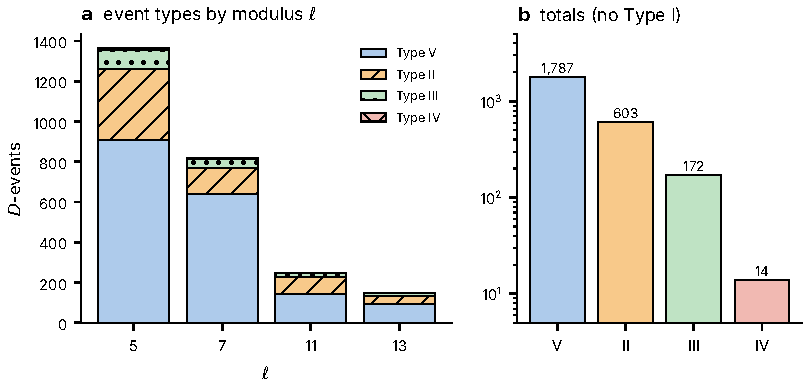
\includegraphics[width=\textwidth]{fig22_event_types}
\caption{\textbf{Event types in the census (finite-exact; $2{,}576$ events, $382$ orbits $x_0=S^2/\ell$ with $L=S$, $G=\ell$; $\ell=5,7,11,13$, $S<1500$, $24$ steps).} (a) Counts of Types V, II, III, IV for each $\ell$ (Type I is absent). (b) Totals $1{,}787$, $603$, $172$, $14$ on a log scale. The census is a finite sample drawn from a fixed parameter box and is not extrapolated.}\label{fig:types}
\end{figure}

\section{Higher-dimensional tower topology}\label{sec:towertop}
The two towers of \cref{sec:towers} give, for each $k$, an occurrence set $D_k=D(x_k)$ and a complex $K_k=K(D_k)$ with $x_k=S_k^2/m$ ($m=11$, $S_k=2^23^{3+k}5^4$, or $m=5$, $S_k=126\cdot2^k$). We study $k\mapsto\beta_i(K_k)$. Four statements are kept apart throughout: the \emph{existence} of an eventual quasi-polynomial law, its \emph{period}, an \emph{effective threshold} after which it holds, and \emph{exact formulas} for the Betti numbers. Only the first two are proved here for all $k$; the last two are finite-exact.

\subsection{Towers are nested filtrations}
\begin{theorem}[nested tower]\label{thm:A5T51}
For $k\le k'$ on either tower: (a) $D_k=\{d\in D_{k'}:d\mid S_k\}$; (b) $K_k$ is the induced subcomplex of $K_{k'}$ on the vertices $D_k$ (the cells of $K_{k'}$ all of whose vertices lie in $D_k$); in particular $K_k\subseteq K_{k+1}\subseteq\cdots$; (c) at every event of the orbit, $x_{8k+7}\to x_{8k+8}$ (resp.\ $x_{3k+2}\to x_{3k+3}$), no cell dies: $\mathrm{Dead}=\emptyset$.
\end{theorem}
\prov{CW-0448}{A5-T5.1}{PROVED}{FULL}
\begin{proof}
(a) $D_k=\{d\mid S_k:d\ge2,\ d\equiv1\ (m)\}$ and $S_k\mid S_{k'}$. (b) For $u,v\in D_k$ every element of $[u,v]^\circ$ divides $\lcm(u,v)\mid S_k$, so $[u,v]^\circ\cap(D_{k'}\cup\{1\})=[u,v]^\circ\cap(D_k\cup\{1\})$ by (a). By \cref{thm:A5T31} $K(D_k)$ and $K(D_{k'})$ have the same edges among $D_k$, hence the same cells with all vertices in $D_k$ (cells are determined by their vertices and $1$-faces). (c) By \cref{thm:R3T5bp,thm:R3T5c} the orbit between $x_{\cdot}$ and the event has $D=D_k$ and then $D=D_{k+1}$; the new occurrences $N=D_{k+1}\setminus D_k$ do not divide $S_k$ and every interval of an edge of $K_k$ consists of divisors of $S_k$, so no edge is pierced (\cref{thm:A5T32}(2)). \qedhere
\end{proof}
\begin{remark}[consequence for homology]
By \cref{thm:cause} and \cref{thm:nested}, along a tower a Betti number is created as relative homology of the new slab and can only be lowered by new cells of one higher dimension. This is why the two towers, which have the same structural form, differ only through the cross-section (the caps of the fixed primes and the lattice $\Lambda$), not through any piercing.
\end{remark}
The nested filtration is drawn in \cref{fig:nestedtowers}.
\begin{figure}[tbp]\centering
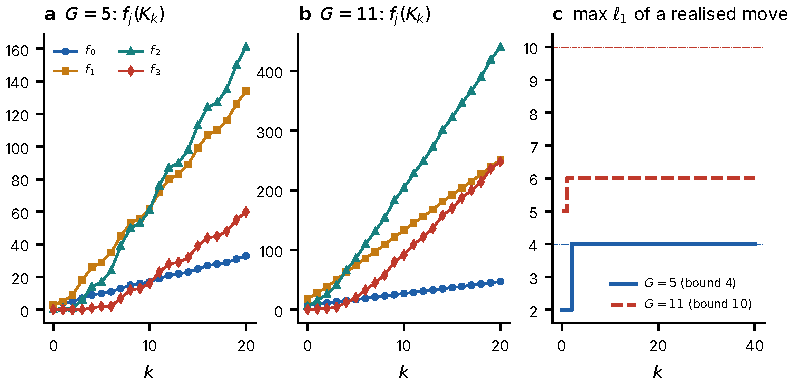
\includegraphics[width=\textwidth]{fig25_nested_towers}
\caption{\textbf{Nested towers (finite-exact; nestedness proved by \cref{thm:A5T51}).} (a), (b) $f$-vectors of $K_k$ for the $G=5$ and $G=11$ towers, $k\le20$ (shown range). (c) Largest $\ell_1$-norm of a realised move for $k\le40$: at most $4$ for $G=5$ and $6$ for $G=11$, below the proved bounds $4$ and $10$ of \cref{lem:A5T52}. Inclusion of cell sets $K_k\subseteq K_{k+1}$ was also verified for all $k\le25$ (both towers). Nothing beyond the computed range is plotted.}\label{fig:nestedtowers}
\end{figure}

\subsection{Stabilisation of moves and the qualitative Betti law}
\begin{lemma}[moves stabilise]\label{lem:A5T52}
Let $\Lambda=\ker(\Z^r\to(\Z/m)^*,\ g\mapsto\prod p_i^{g_i})$ for the primes $p_i$ of $S_k$. Every region-Graver vector $g$ satisfies $\|g\|_1\le|\langle p_1,\dots,p_r\rangle|\le\varphi(m)$. Hence all moves of the towers have $\ell_1$-norm at most $10$ ($m=11$) resp.\ $4$ ($m=5$), and once the cap of the growing prime exceeds this bound the set of moves of $K_k$ does not change with $k$.
\end{lemma}
\prov{CW-0449}{A5-T5.2}{PROVED}{FULL}
\begin{proof}
A region-Graver vector is minimal in $\Lambda\cap[-q,q]$; every $h\sqsubseteq g$ lies in the box, so $g$ is a Graver vector of $\Lambda$. Because $g$ has a fixed sign in each coordinate, $g$ is the sequence $a_1,\dots,a_n$ ($n=\|g\|_1$) consisting of $g_i^+$ copies of $p_i$ and $g_i^-$ copies of $p_i^{-1}$ in the group $H=\langle p_i\rangle\le(\Z/m)^*$, with product $1$, and minimality says that it has no proper non-empty zero-sum sub-sequence. The partial products $s_j=a_1\cdots a_j$ ($1\le j\le n-1$) are $\ne1$ (a prefix would be a zero-sum subsequence) and pairwise distinct (a quotient $s_j/s_i$ would be one), so $n-1\le|H|-1$. For $m$ prime $\varphi(m)=m-1$. \qedhere
\end{proof}
\begin{theorem}[eventual quasi-polynomial Betti laws, qualitative]\label{thm:A5T53}
Let $\rho$ be the growing prime ($\rho=3$, $m=11$; $\rho=2$, $m=5$), $\omega=\ord_m(\rho)$ ($\omega=5$, resp.\ $4$). For every field $\mathbb k$ and every $i\ge0$ there exist an integer $k_1$ and a quasi-polynomial $q_i$ of degree $\le1$ and period dividing $\omega$ such that $\beta_i(K_k;\mathbb k)=q_i(k)$ for all $k\ge k_1$. The threshold $k_1$ is \emph{not} controlled.
\end{theorem}
\prov{CW-0450}{A5-T5.3}{PROVED-SCOPED}{SPLIT}
\begin{proof}[Proof (structure; the threshold is not effective)]
Use the coordinates $(u,h)\in\Z^{r-1}\times\Z$ with $h$ the exponent of $\rho$, and let $\Lambda'$ be the lattice. Let $\tilde K$ be the complex defined by the interval rule on the infinite slab $\Lambda'\cap(\text{box}\times\N)$ \emph{including the origin as a vertex}; $K_k$ is the subcomplex of cells avoiding the origin and of height $\le h_0+k$ (an edge between non-origin vertices has an interval of lower height, so the rule is the same). Since $\rho^\omega\equiv1$, the shift $T:(u,h)\mapsto(u,h+\omega)$ preserves $\Lambda'$, and the lattice points of the shifted box are the shifts of those of the box, so $T$ is an injective cellular map; a cell whose minimal height is at least $\omega$ is the image under $T$ of a cell of $\tilde K$ (if the preimage box meets the origin, $T$ of the origin is a lattice point of the shifted box, so the origin is then a vertex of the preimage cell). By \cref{lem:A5T52} cells have bounded diameter, hence the cells of $\tilde K$ that are not in the image of $T$ form a finite set. Form $R=\bigoplus_hC_*(K_h)$ as a graded module over $\mathbb k[t,T]$, $t$ acting by inclusion $K_h\to K_{h+1}$ (degree $1$) and $T$ by the shift (degree $\omega$); it is finitely generated by the above finite set of cells (and the shifts of the finitely many cells through the origin). By Noetherianity $\bigoplus_hH_i(K_h)=H_i(R)$ is a finitely generated graded module, and the Hilbert function of a finitely generated graded module over $\mathbb k[t,T]$ with weights $(1,\omega)$ is eventually a quasi-polynomial of degree $\le1$ and period dividing $\omega$ (Hilbert--Serre; \cite{Eisenbud1995}; for quasi-polynomials in this form \cite{Stanley1997,Ehrhart1962}). \qedhere
\end{proof}
\begin{corollary}[conditional exact formulas]\label{cor:cond}
If for the $G=11$ tower the regime of $\beta_1$ (resp.\ $\beta_2$, $\beta_3$) begins at some $k_1\le130$, then $\beta_1\equiv8$ and $\beta_2\equiv17$ for all $k\ge k_1$, resp.\ $\beta_3(k+5)=\beta_3(k)+9$ for all $k\ge\max(k_1,8)$. The unconditional statement needs a bound on $k_1$ (a regularity bound for the module $H_i(R)$), which is open.
\end{corollary}
\begin{proof}
A quasi-polynomial of degree $\le1$ and period $5$ is determined by two values in each residue class. Between $k_1$ and $140$ there are at least $10$ computed consecutive values, in each residue class at least two, on which the computed laws of \cref{thm:A5T6} hold. \qedhere
\end{proof}
\begin{remark}[four distinctions]
(i) \emph{Existence} of an eventual quasi-polynomial: proved (\cref{thm:A5T53}). (ii) \emph{Period}: divides $\omega$: proved. (iii) \emph{Effective threshold} $k_1$: not known; the observed onset ($k=2$ for $\beta_1$, $k=6$ for $\beta_2$, $k=8$ for $\beta_3$ on $G=11$; $k=7$ on $G=5$) is a computed fact for $k\le140$. (iv) \emph{Exact formulas}: finite-exact to $k\le140$, and exact for all $k$ only under the hypothesis of \cref{cor:cond}. The formulas are not promoted to universal ones.
\end{remark}

\subsection{Contrast: corrected \texorpdfstring{$\sigma$}{sigma}-transport versus collective monotonicity}\label{ssec:contrast}
The \emph{collective} map is monotone: $D(x)\subseteq D(C(x))$ (\cref{lem:M}), so occurrences persist and the complex only changes by the transition law. The \emph{generative} SELECT-II edges $m\xrightarrow{N}m'=m(N+1)^2/N$ ($N\mid m$) behave differently, and the claim of inclusion for them must not be carried over.
\begin{proposition}[corrected $\sigma$-transport, B2-T9]\label{prop:B2T9}
On every SELECT-II edge $\sigma(m')=\sigma(m)(N+1)/c$ with $c=\prod_{p\mid N}p^{l_p}$ and $c\le N$. Hence $\sigma$ \emph{strictly increases}, $\sigma(m')>\sigma(m)$, and $D(m')\ne D(m)$ (since $\sigma=\max D$): no step is silent. It is \emph{not} true that $D(m)\subseteq D(m')$ or that $\sigma(m)\mid\sigma(m')$: the edge $4\xrightarrow{2}18$ has $D(4)=\{2\}$, $D(18)=\{3\}$.
\end{proposition}
\prov{CW-0403}{B2-T9}{CORRECTED}{CORRECTED}
\begin{proof}
The transport formula is \cref{thm:B2T2}. Since $l_p\le v_p(N)$, $c\le N<N+1$. For the example: $4=2^2$ has $\sigma=2$; $18=2\cdot3^2$ has $\sigma=3$. \qedhere
\end{proof}
\begin{remark}[finite-exact check]
On all $24{,}496$ edges with $1\le m\le3000$, $N\mid m$: the transport formula holds, $\sigma$ strictly increases and $D$ changes on every edge; the inclusion $D(m)\subseteq D(m')$ holds on $13{,}894$ edges and fails on $10{,}602$ (the first failure is $m=4$, $N=2$). A table of the $24{,}495$ edges with $m\ge2$ in the inherited note differs from this count only by the edge $1\to4$ (\stat{finite-exact}). Nothing in this paper uses inclusion on generative edges, and no Graver-basis monotonicity claim is made.
\end{remark}
\begin{remark}[what this does to the comparison]
The contrast is part of why the hierarchy of \cref{sec:corr} is kept level by level: a statement that holds along collective orbits (persistence of occurrences, nested towers) need not hold along generative histories.
\end{remark}

\subsection{Exact tower laws to \texorpdfstring{$k\le140$}{k<=140}}\label{ssec:towerlaws}
\begin{theorem}[tower laws; finite-exact]\label{thm:A5T6}
The following were computed exactly (over $\mathbb F_2$ and over $\mathbb F_p$, $p=2^{31}-1$, which gave the same Betti vector at every $k$) for every $k\le140$ and are \emph{not} extrapolated.
\begin{enumerate}[label=(\alph*),itemsep=1pt]
\sloppy\item $G=11$: $\beta_0=1$; $\beta_1=6,7,8,8,8,\dots$ ($=8$ for $2\le k\le140$); $\beta_2=0,1,4,7,13,16,17,17,\dots$ ($=17$ for $6\le k\le140$); $\beta_3=0$ for $k\le8$ and $\beta_3(k+5)=\beta_3(k)+9$ for $8\le k\le135$, with $(\beta_3(8),\dots,\beta_3(12))=(0,4,4,7,8)$; $\beta_4=0$. Moreover $|D_k|=2k+7$ (proved, \cref{thm:R3T5bp}).
\item $G=5$: $(\beta_0,\beta_1,\beta_2,\beta_3)=(1,1,0,0),\allowbreak(1,1,0,0),\allowbreak(1,4,0,0),\allowbreak(1,6,0,0),\allowbreak(1,6,1,0),\allowbreak(1,6,1,0),\allowbreak(1,6,3,0)$ for $k=0,\dots,6$ and $(1,6,5,0)$ for every $7\le k\le140$.
\item The event at the orbit step $5\to6$ of the $G=5$ tower, which is the tower-index step $k=1\to2$ (not ``$5\to6$'' in the index $k$), adds one occurrence ($56$), four new edges to old vertices, no dead cell and no new $2$-cell, $f=(4,5,1)\to(5,9,1)$, and $\beta_1$ passes from $1$ to $4$; this is the star formula $\Delta\beta_1=4-1=3$ of \cref{thm:A5T44}.
\end{enumerate}
\end{theorem}
\prov{CW-0451}{A5-T6}{FINITE-EXACT}{FINITE}
\begin{proof}[Computation]
Both towers were generated from the closed forms of \cref{thm:R3T5bp,thm:R3T5c}, the complexes $K(D_k)$ were built with the interval rule and the Betti numbers computed by exact linear algebra over both fields, with the check $\partial^2=0$ over $\F_2$ at every $k$; the closed forms for $|D_k|$ were checked at every $k$. The full tables are in Appendix~\ref{app:towers}. \qedhere
\end{proof}
The computed Betti numbers of the two towers are plotted in \cref{fig:g5betti,fig:g11betti}.
\begin{figure}[tbp]\centering
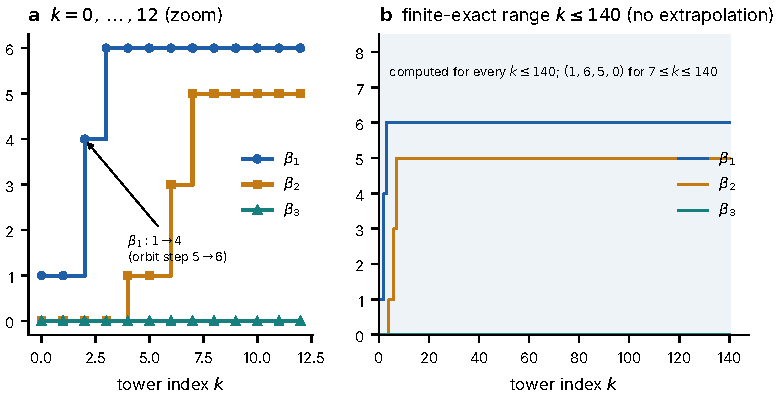
\includegraphics[width=\textwidth]{fig23_g5_betti}
\caption{\textbf{Betti numbers of the $G=5$ tower (finite-exact; \cref{thm:A5T6}).} $S_k=126\cdot2^k$. (a) $\beta_1,\beta_2,\beta_3$ for $k=0,\dots,12$; the jump $\beta_1:1\to4$ is at tower index $k=1\to2$ (orbit step $5\to6$). (b) the whole computed range $k\le140$ (shaded); the values $(1,6,5,0)$ hold for every computed $7\le k\le140$. No curve is extended beyond $k=140$.}\label{fig:g5betti}
\end{figure}
\begin{figure}[tbp]\centering
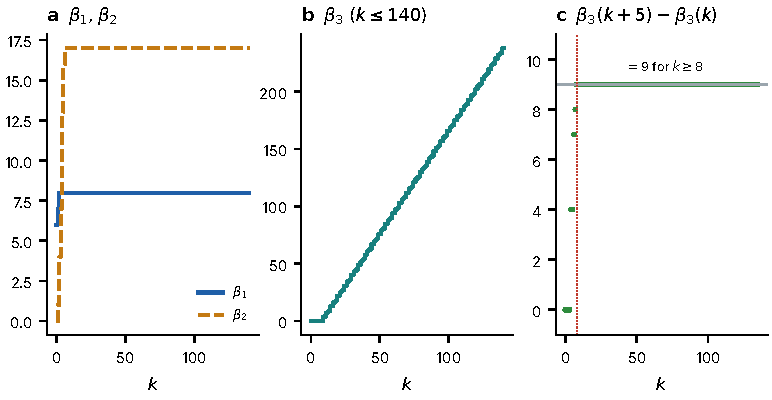
\includegraphics[width=\textwidth]{fig24_g11_betti}
\caption{\textbf{Betti numbers of the $G=11$ tower (finite-exact; \cref{thm:A5T6}).} $S_k=2^2\,3^{3+k}\,5^4$, computed for every $k\le140$. (a) $\beta_1,\beta_2$ (stable at $8$ and $17$). (b) $\beta_3$. (c) the increment $\beta_3(k+5)-\beta_3(k)$, equal to $9$ for all computed $k\ge8$. The periodic structure of period $5$ is that of $\ord_{11}(3)=5$ (a proved arithmetic fact), the values are computed.}\label{fig:g11betti}
\end{figure}
\begin{proposition}[comparison of the two towers; finite-exact and open]\label{prop:A4T56}
Both towers are nested with $\mathrm{Dead}=\emptyset$ (\cref{thm:A5T51}) and have exactly one occurrence event per period, but the Betti vectors differ: $G=5$ is bounded with $\beta_3=0$, $G=11$ has $\beta_3$ growing linearly in $k$ over the computed range. The scaling laws $x_{n+3}=4x_n$ and $x_{n+8}=9x_n$ determine $D$ and hence the realised complex, but not the dormant relations and not the Betti pattern; the stabilisation scale is set by the Graver bound ($4$ versus $10$) and by $\omega$ ($4$ versus $5$) (\cref{lem:A5T52,thm:A5T53}). \emph{No theorem here explains why $G=11$ has growing $\beta_3$ while $G=5$ has none}; this is open (\cref{sec:concl}). The $\ell=29$ tower stays finite-exact (\cref{ex:l29}).
\end{proposition}
\prov{CW-0434}{A4-T5}{MIXED}{SPLIT}
\prov{CW-0435}{A4-T6}{FINITE-EXACT}{FINITE}

\section{Restricted correspondences and obstructions}\label{sec:corr}
Two integer systems act on the same states: the collective map $C$ and the generative \emph{SELECT-II} edges~\cite{FoundI} $T_N:m\mapsto m(N+1)^2/N$ ($N\mid m$). This section records what can be compared exactly between them. The comparison is graded by levels, and \emph{a level is never inferred from a weaker one}.

\begin{definition}[levels of correspondence]\label{def:levels}
\textbf{L1} (numerical): the two systems relate the same pair of states, or the same ratio $x_m/x_n$. \textbf{L2} (occurrence information): equal initial and final occurrence structures. \textbf{L3} (reduced event records): equal numbers (and, for integers, equal $\sigma$-sequences) of occurrence-changing steps along the two paths. \textbf{L4} (geometric structures): equal realised complexes along the paths. \textbf{L5} (dynamical intertwining): a map conjugating the two dynamics. The hierarchy runs L1 $\to$ L2 $\to$ L3 $\to$ L4 $\to$ L5 in increasing strength; each level is tested on its own.
\end{definition}

\subsection{Transport along a SELECT-II edge}
\begin{theorem}[box transport, B2-T2]\label{thm:B2T2}
Let $m\xrightarrow{N}m'=m(N+1)^2/N$ with $N\mid m$, and let $p$ be a prime, $n=v_p(N)$, $w=v_p(N+1)$ (at most one of $n,w$ is non-zero). Then $q_p(m')=q_p(m)+w$ if $p\nmid N$, and $q_p(m')=q_p(m)-l_p$ if $p\mid N$, where $l_p=\lfloor n/2\rfloor$ if $v_p(m)$ is odd and $l_p=\lceil n/2\rceil$ if $v_p(m)$ is even. Consequently $\sigma(m')=\sigma(m)(N+1)/c$ with $c=\prod_{p\mid N}p^{l_p}\le N$.
\end{theorem}
\prov{CW-0396}{B2-T2}{PROVED}{FULL}
\begin{proof}
$v_p(m')=v_p(m)+2w-n$. For $p\nmid N$ ($n=0$) the change $2w$ is even, so $\lfloor v_p/2\rfloor$ increases by $w$. For $p\mid N$ ($w=0$), put $e=v_p(m)\ge n$: $\lfloor(e-n)/2\rfloor=\lfloor e/2\rfloor-\lfloor n/2\rfloor$ if $e$ is odd and $\lfloor e/2\rfloor-\lceil n/2\rceil$ if $e$ is even. Multiplying over primes, $\prod_{p\mid N+1}p^{w}=N+1$ and $c\le\prod p^{n}=N$. \qedhere
\end{proof}
\begin{theorem}[gain--loss balance, B2-T3]\label{thm:B2T3}
For a history with labels $N_1,\dots,N_r$ put $G_p=\sum_iv_p(N_i+1)$ and let $\Lambda_p$ be the total decrease of $q_p$ over the steps with $p\mid N_i$. Then $q_p(\mathrm{end})-q_p(\mathrm{start})=G_p-\Lambda_p$, so the loss budget $\Lambda_p$ is determined by the content and the endpoints, not by the order. If two admissible blocks $u,v$ from the same state have equal endpoints, then
\[
\Lambda_p(u)-\Lambda_p(v)=\tfrac12\big(H_p(u)-H_p(v)\big),\qquad H_p=\sum_iv_p(N_i)\ \text{(denominator content).}
\]
\end{theorem}
\prov{CW-0397}{B2-T3}{PROVED}{FULL}
\begin{proof}
Telescope \cref{thm:B2T2}. The multiplier of a history is $\prod_i(N_i+1)^2/N_i$; equal endpoints from the same state force $2G_p(u)-H_p(u)=2G_p(v)-H_p(v)$ for every $p$, and substituting $G_p=\Delta q_p+\Lambda_p$ (with $\Delta q_p$ equal for $u$ and $v$) gives the relation. \qedhere
\end{proof}
\begin{theorem}[parity conservation, restricted]\label{thm:B2T4}
Let every label of a history satisfy $v_p(N)\le1$ and let $c$ be the number of labels divisible by $p$. Then the parity of $v_p$ flips at each of these $c$ edges and is unchanged at the others. The $p$-edges therefore see the parities $\pi,\pi+1,\pi,\dots$ in order ($\pi$ the parity of $v_p$ at the start), and the loss steps for $p$ are those that see an even parity: their number is $\lceil c/2\rceil$ if $\pi$ is even and $\lfloor c/2\rfloor$ if $\pi$ is odd, whatever the order of the labels. Orderings only permute when the losses occur. No claim is made outside $v_p(N)\le1$.
\end{theorem}
\prov{CW-0398}{B2-T4}{PROVED-SCOPED}{FULL}
\begin{proof}
For $p\mid N$ with $n=v_p(N)=1$ we have $w=0$ and $v_p(m')=v_p(m)-1$, so the parity flips; for $p\nmid N$, $v_p(m')=v_p(m)+2w$, so it does not. By \cref{thm:B2T2}, $l_p=\lfloor1/2\rfloor=0$ if $v_p(m)$ is odd and $l_p=\lceil1/2\rceil=1$ if $v_p(m)$ is even; a loss for $p$ is therefore a $p$-edge taken at even $v_p(m)$. The alternation of parities gives the count. \qedhere
\end{proof}
\begin{remark}[correction of wording]
The inherited summary describes the loss step as the one with $v_p(m)$ odd; by \cref{thm:B2T2} it is the one with $v_p(m)$ even (for $n=1$ an odd exponent loses nothing). The parity-flip conclusion is unaffected.
\end{remark}

\subsection{Rigid relations and one-step obstructions}
\begin{proposition}[one-step obstruction]\label{prop:onestep}
For every state $x$ with $D(x)\ne\emptyset$, $1<C(x)/x\le2$, whereas $T_N(x)/x=R(N):=(N+1)^2/N\ge4$ for every $N\ge1$. Hence $C(x)\ne T_N(x)$ for all $N$: one collective step is never a SELECT-II edge.
\end{proposition}
\begin{proof}
$C(x)/x=1+L^2/(ah)$ and $L^2\mid a$, $h\ge1$ give $L^2/(ah)\le1$. $R(N)=N+2+1/N\ge4$ with equality iff $N=1$. \qedhere
\end{proof}
\begin{theorem}[snapshot relation, B-T12]\label{thm:BT12}
On the rigid domain (\cref{thm:B2T6}, $t\in\{1,2,3\}$, $G=1$) $C^3(x)=4x=T_1(x)$. This relation holds at the snapshots $n\equiv0\pmod3$ only: by \cref{prop:onestep} no single collective step equals a SELECT-II edge, so the relation is \emph{not} a conjugacy of the two systems (no L5).
\end{theorem}
\prov{CW-0394}{B-T12}{PROVED}{FULL}
\begin{proof}
\Cref{thm:B2T6} and $T_1(x)=4x$; the second part is \cref{prop:onestep}. The identity $C^3=4x$ was also checked on $90$ integers of the rigid domain (\stat{finite-exact}). \qedhere
\end{proof}
\begin{theorem}[rigid event correspondence, B2-T10]\label{thm:B2T10}
Let $x=t\sigma^2$, $t\in\{1,2,3\}$, $\sigma$ even. The collective orbit passes from $x$ to $C^3(x)=4x$ with reduced $\sigma$-sequence $(\sigma,2\sigma)$, one birth event and $\tau(\mu)$ new occurrences, $\sigma=2^a\mu$, $\mu$ odd; the single edge $T_1:x\mapsto4x$ has the same $\sigma$-sequence, one birth event and the same number $\tau(\mu)$ of new occurrences. L3 holds. L4 holds at the integer endpoints by \cref{thm:B2T1}; L5 does not (\cref{thm:BT12}).
\end{theorem}
\prov{CW-0404}{B2-T10}{PROVED}{FULL}
\begin{proof}
For $\sigma$ even $G=1$, so \cref{thm:B2T6} applies: the carry occurs at the third step ($t=3\to1$, $u=2$) and $D$ changes only there, with $\tau(2\sigma)-\tau(\sigma)=\tau(\mu)$ new elements (\cref{thm:B2T8}). The edge $T_1$ sends $\sigma\to2\sigma$ ($c=1$, $N+1=2$) with the same count. By \cref{thm:B2T1} the box record of an integer is a function of $\sigma$. \qedhere
\end{proof}
\begin{theorem}[a coincidence family, B2-T12]\label{thm:B2T12}
Let $N=2^a-1$ be squarefree ($a\ge2$), $s$ even, $x=Ns^2$. Then $C^k(x)=T_N(x)=(2^as)^2$ with $k=1+3a/2$ for $a$ even and $k=1+2+3(a-1)/2$ for $a$ odd: $k$ collective steps against exactly one SELECT-II event.
\end{theorem}
\prov{CW-0406}{B2-T12}{PROVED}{FULL}
\begin{proof}
$N$ squarefree gives $\sigma(x)=s$, $t=N$, and $G=1$ since $s$ is even. $T_N(x)=x(N+1)^2/N=(2^as)^2$. For $a$ even, $t+1=2^a$ is a square: $t\to1$, $\sigma\to2^{a/2}s$ in one step; each rigid period $(1,2,3)$ takes three steps and doubles $\sigma$, and $a/2$ periods give $\sigma=2^as$ with $t=1$: $k=1+3a/2$. For $a$ odd, $\sqf(2^a)=2$: $t\to2$, $\sigma\to2^{(a-1)/2}s$; two more steps ($t=2\to3\to1$) double $\sigma$; $(a-1)/2$ further periods are needed: $k=1+2+3(a-1)/2$. \qedhere
\end{proof}
\begin{remark}[finite-exact]
Verified for $a=2,\dots,5$ and $s\in\{2,4,6,8,10\}$ ($k=4,6,7,9$) with the engine; a scan of $x<4000$ in the source found all single-edge coincidences with $N+1\in\{2^a,3\cdot2^a\}$; completeness is \stat{open} and not claimed.
\end{remark}
\begin{theorem}[scaling obstruction, B2-T13]\label{thm:B2T13}
(a) $R(N)=(N+1)^2/N$ is an integer iff $N=1$ (then $R=4$). (b) The multiplier $9$ of the $G=11$ tower is not $R(N)$ for any integer $N$ ($R(N)=9\iff N^2-7N+1=0$, no integer root), and it is not a product of two or more factors $R(N_i)$, since each factor is $\ge4$ and such a product is $\ge16$. (c) The multiplier $900$ of the $\ell=29$ example is not $R(N)$ for any integer $N$.
\end{theorem}
\prov{CW-0407}{B2-T13}{PROVED}{FULL}
\begin{proof}
(a) $\gcd(N,(N+1)^2)=1$, so $R(N)$ is reduced with denominator $N$. (b) $(N+1)^2=9N$ is $N^2-7N+1=0$, with discriminant $45$, not a square; the product bound follows from $R(N)\ge4$ (as $R(N)=N+2+1/N$). (c) $(N+1)^2=900N$ is $N^2-898N+1=0$ with discriminant $898^2-4=806{,}400=896\cdot30^2$, and $896=2^7\cdot7$ is not a square. \qedhere
\end{proof}
\Cref{fig:hierarchy} summarises the hierarchy of levels and the scaling obstruction.
\begin{figure}[tbp]\centering
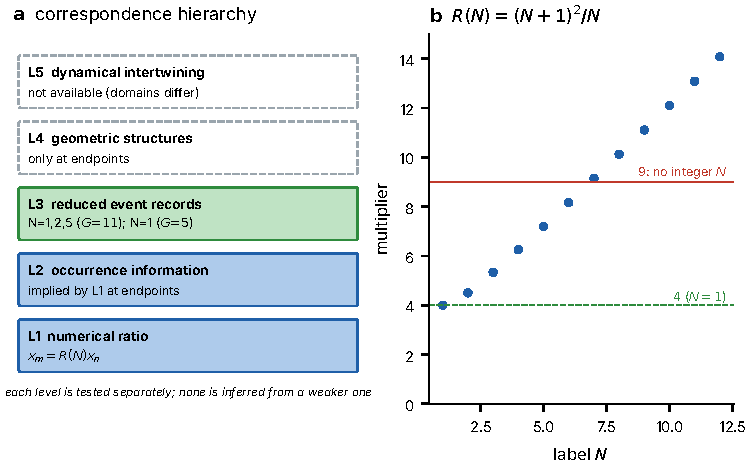
\includegraphics[width=\textwidth]{fig26_hierarchy_obstruction}
\caption{\textbf{The hierarchy and the scaling obstruction (schematic left; exact right).} (a) Levels of correspondence L1--L5 with what is established: L3 for the formal multipliers $N=1,2,5$ ($G=11$) and $N=1$ ($G=5$) at the event level; L4 only at endpoints; L5 not available. The diagram is schematic and each level is tested separately. (b) $R(N)=(N+1)^2/N$ for $N=1,\dots,12$; the integer value $4$ occurs only at $N=1$ and $9$ occurs for no integer $N$ (proved by \cref{thm:B2T13}).}\label{fig:hierarchy}
\end{figure}

\subsection{Formal multipliers on the two towers}
\begin{theorem}[classification of multiplier coincidences, R3-T7]\label{thm:R3T7}
Write the iterates of a tower as $x_n=u\,\rho^{2a}x_0$ with $u\in[1,P]$ ($(P,\rho^2)=(8,9)$ for $G=11$, $(3,4)$ for $G=5$). A pair $n<m$ has $x_m/x_n=R(N)$ for an integer $N$ exactly in the following cases ($x_m/x_n=\rho^{2a}v/u$, $a$ the number of periods crossed, $u,v\in[1,P]$):
\begin{enumerate}[label=(\alph*),itemsep=1pt]
\item $G=11$: $N=1$, $(u,a,v)\in\{(1,0,4),(2,0,8)\}$ (ratio $4$); $N=2$, $(u,a,v)=(2g,1,g)$, $g=1,\dots,4$ (ratio $9/2$); $N=5$, $(5,1,4)$ (ratio $36/5$); $N=8$, $(8,2,1)$ (ratio $81/8$). No other pair has a SELECT-II ratio.
\item $G=5$: $N=1$, $(u,1,u)$ (ratio $4$, a full period); $N=3$, $(3,2,1)$ (ratio $16/3$).
\end{enumerate}
At the event level, with L3 meaning that the number of occurrence-changing steps along the collective segment, which is $a$, equals that of the formal edge, which is $1$ if $D(x_n)\ne D(x_m)$ and $0$ otherwise (that is, $[a\ge1]$): L3 holds for $N=1,2,5$ ($G=11$; for $N=1$ both counts are $0$: the formal $T_1$ is \emph{silent} on these rational states) and for $N=1$ ($G=5$); L3 fails, although L1 holds, for $N=8$ ($G=11$; $a=2$ against $1$) and for $N=3$ ($G=5$; $a=2$ against $1$). The full-period multiplier is $4=R(1)$ for $G=5$ and $9$ for $G=11$, which is not of the form $R(N)$ (\cref{thm:B2T13}).
\end{theorem}
\prov{CW-0422}{R3-T7}{PROVED}{FULL}
\begin{proof}
By \cref{thm:R3T5bp,thm:R3T5c}, $x_{Pk+j}=(j+1)\rho^{2k}x_0$ for $0\le j<P$. Write $x_n=u\rho^{2a_n}x_0$, $x_m=v\rho^{2a_m}x_0$ with $a=a_m-a_n$. The equation $\rho^{2a}v/u=(N+1)^2/N$ is $N\rho^{2a}v=u(N+1)^2$. As $\gcd(N,N+1)=1$, $N\mid u$, so $N\le P$ and $u=Nw$ with $\rho^{2a}v=w(N+1)^2$, $1\le v\le P$, $1\le w\le\lfloor P/N\rfloor$. For $G=11$ ($P=8$, $\rho^2=9$) one checks $N=1,\dots,8$: $9^av=w(N+1)^2$ has the solutions listed (e.g.\ $N=2$: $9^av=9w$ forces $a=1$, $v=w$; $N=8$: $9^av=81$ forces $a=2$, $v=1$; $N=3,4,6,7$ have none because $16w,25w,49,64$ are not of the form $9^av$ with $1\le v\le8$), and similarly for $G=5$ ($P=3$, $\rho^2=4$, $N\le3$). Events: $D$ changes exactly at the steps $x_{Pk}$, $k\ge1$ (\cref{thm:R3T5bp,thm:R3T5c}), so the collective segment from $x_n$ to $x_m$ crosses exactly $a$ of them, and $D(x_n)\ne D(x_m)$ iff $a\ge1$. \qedhere
\end{proof}
\begin{remark}[finite-exact check; phase shift]
Brute force over the first $41$ iterates ($G=11$) and $19$ iterates ($G=5$) found exactly these cases, with $10,17,4,4$ pairs for $N=1,2,5,8$ ($G=11$) and $16,5$ pairs for $N=1,3$ ($G=5$), and the event counts $0,1,1,2$ and $1,2$ respectively (\stat{finite-exact}). A phase-shifted correspondence holds on the $G=11$ tower: $C^{8-g}(2gS^2/11)=\tfrac92\cdot2gS^2/11$ for $g=1,\dots,4$ (the formal edge $N=2$, $R(2)=9/2$), verified for $S=S_0$; the multiplier $9$ itself is not representable. The $\sigma$-track step of one period ($L:S_k\to3S_k$) is realised by a genuine integer edge ($m=2S_k^2\xrightarrow{2}9S_k^2$) with multiplier $9/2$ rather than $9$. These are statements about L1--L3 only; no L4 beyond endpoints and no L5 is claimed.
\end{remark}

\subsection{Corrected block and cited results}
\begin{proposition}[the SELECT-II block, B2-T14 (split)]\label{prop:B2T14}
(i) \emph{Common carrier} (proved): the generative edge acts on $\sigma$ by $\sigma\mapsto\sigma(N+1)/c$ (\cref{thm:B2T2}), and the collective regime-I carry by $\sigma\mapsto\sigma u$ (\cref{thm:B2T6}); both are rules on the same object, but with unrelated multipliers, meeting only in the rigid case, the coincidence family and the $N=1$ obstruction. (ii) \emph{Level 3 $\Rightarrow$ level 4 for integers} (proved): the box record of an integer state is a function of $\sigma$ (\cref{thm:B2T1}), so equal $\sigma$-sequences give equal geometric records. (iii) \emph{Loss-budget blindness} (\stat{cited}, finite-exact): the geometric events of a history do not see the loss budget $\Lambda$; this part rests on inherited computations and is not re-derived.
\end{proposition}
\prov{CW-0408}{B2-T14}{PROVED}{SPLIT}
\begin{remark}[cited]
The following inherited records are \stat{cited}, with ownership as in Appendix~\ref{app:crosswalk}: B2-T5 (mixed-index forcing, proved for contents $2^\alpha3^\beta$ and open for $k>2$ primes), B2-T11 (birth-endpoint classification $x_m=4^jx_n$; finite-exact on $16{,}028$ pairs, not re-run), and, from Paper~II~\cite{PaperII}, R3-T3, R3-T3$'$, R3-T4 and the obstruction A4-T7, discussed below.
\end{remark}
\prov{CW-0399}{B2-T5}{MIXED}{CITED}
\prov{CW-0405}{B2-T11}{PROVED}{CITED}
\prov{CW-0413}{R3-T3}{PROVED}{CITED}
\prov{CW-0414}{R3-T3'}{FINITE-EXACT}{CITED}
\prov{CW-0415}{R3-T4}{PROVED-SCOPED}{CITED}
\begin{proposition}[obstruction to identifying histories with orbits, A4-T7; cited from Paper~II]\label{prop:A4T7}
The move complex of an integer state is contractible (\cref{thm:B2T1}), whereas the history complexes of Paper~II between integer endpoints have two or three components in the cases studied there; consequently no identification of the two kinds of complex is available, and no map between them is claimed. The connection beyond this obstruction is \stat{open}.
\end{proposition}
\prov{CW-0436}{A4-T7}{MIXED}{CITED}
\begin{remark}[no universal correspondence]
Nothing in this section establishes a universal law relating the two systems. What is exact: the transport formulas, the one-step and scaling obstructions, the rigid relation at snapshots, one coincidence family and the classification on two towers. The strongest levels are not inferred from the weaker ones.
\end{remark}

\section{Conclusions and open problems}\label{sec:concl}
\subsection{What has been established}
The central question was which geometry changes along a collective orbit are exactly predictable from the arithmetic state, which depend on additional relations, and which topological consequences need cellular-attachment data. The answer assembled here is as follows.
\begin{itemize}[itemsep=2pt]
\item \emph{Exactly determined by the arithmetic state.} The realised complexes are functions of the occurrence set $D$ (\cref{thm:R3T1a,thm:A5T31}); for integers they collapse to the single integer $\sigma$ and are contractible (\cref{thm:B2T1}); occurrences are monotone along orbits (\cref{lem:M}); the next occurrence event is given by one linear congruence per candidate (\cref{thm:sieve,cor:event}) and events never stop (\cref{cor:never}); the old edges that die and the new edges that appear are read from divisor intervals (\cref{thm:A5T32}).
\item \emph{Depending on additional relations.} Equal occurrence sets can carry different primitive relations (\cref{thm:R3T1,thm:R3T2}); relations can be dormant and become active without being created (\cref{thm:A4T1,thm:A4T2}); whether an activated target lies on the orbit is a reachability question with a proved obstruction and exact finite examples (\cref{thm:A5T11,thm:A4T3c,thm:A4T3c375}).
\item \emph{Needing cellular-attachment data.} The change of Betti numbers follows the zig-zag identity, with local terms and global ranks (\cref{thm:zigzag}); a change always has a cause in dead or new cells (\cref{thm:cause}); at graph level the update is exact (\cref{thm:A5T44}); activation does not force a topological change and does not always raise homology (\cref{prop:A4T4c,thm:A5T7}).
\item \emph{Towers.} Both towers are nested with no dead cell (\cref{thm:A5T51}); an eventual quasi-polynomial law exists with period dividing the order of the growing prime, with uncontrolled threshold (\cref{thm:A5T53}); the exact laws are finite-exact to $k\le140$ and are not promoted (\cref{thm:A5T6}).
\item \emph{Correspondences.} Between the collective and the generative systems the exact statements are transport formulas, the snapshot relation $C^3=4x=T_1(x)$, the one-step and scaling obstructions, a coincidence family and the classification of formal multipliers on the two towers; no universal correspondence is established (\cref{sec:corr}).
\end{itemize}
Corrections carried out in this paper are the following: in B2-T7 only $G_\infty=1\Rightarrow$ rigidity holds, the $G=5$ tower being a counterexample to the converse (\cref{prop:B2T7}); in B2-T9, $\sigma$ strictly increases and $D$ changes on every edge, but inclusion $D(m)\subseteq D(m')$ fails (\cref{prop:B2T9}); the inherited proof of the cause criterion was repaired (\cref{thm:cause}); the loss step of B2-T4 is the even one (\cref{thm:B2T4}); the entry-time statistic for the regime-I descent is $12$ in the range checked (\cref{rem:entry}).

\subsection{Limits of this paper}
All census and tower results are finite-exact and are stated with their ranges; no extrapolated curve is plotted. Inherited verifier suites and inherited censuses (the $993$-pair reachability table, the $474$-event table, the census of $1{,}920$ orbits, the $20{,}000$-candidate rigid sample, the $16{,}028$-pair birth-endpoint scan) are \stat{cited} and not re-run. The ownership of results shared with Paper~II is recorded in Appendix~\ref{app:crosswalk}. The programme sources~\cite{FoundI,GEOI} are cited at their pinned commits and were not re-fetched.

\subsection{Open problems}
\begin{enumerate}[label=\textbf{P\arabic*.},itemsep=2pt]
\item \emph{Relations beyond $D$} (\cref{prob:R3T2p}): classify the minimal descriptor $\Phi(D,J)$ for boxes $q\ne\mathbf 1^k$ and three or more primes.
\item \emph{Reachability} (\cref{prob:A4T3f}): are infinitely many members of the activation family on the orbit of their source? Is every non-blocked member reached? A closed form for the landing step?
\item \emph{Type predicate}: no arithmetic predicate of the state is known that predicts the type (V, II, III, IV) of an occurrence event; only the form of the answer, determined by $(K(D),N)$, is proved (\cref{thm:A5T7}).
\item \emph{Dead edges and $\beta_1$}: in the census no event with a dead edge raises $\beta_1$; in the abstract calculus it can (\cref{cx:abstract}); can it along a collective orbit?
\item \emph{Higher-dimensional predictor}: a rebuild-free prediction of the Betti vector when $2$-cells and higher cells are present (\cref{thm:A5T44} is graph-level only).
\item \emph{Threshold and mechanism for the towers}: an effective bound for $k_1$ in \cref{thm:A5T53}; an explanation of why $G=11$ has growing $\beta_3$ and $G=5$ none (\cref{prop:A4T56}).
\item \emph{Periodicity}: is the stage sequence periodic for every persistent orbit? For $\ell=29$ the periodic pair $(P,\rho^2)=(35,900)$ is verified, not proved (\cref{ex:l29}); the $(3,4),(8,9),(35,900)$ census is not a theorem.
\item \emph{Mixed-index forcing for $k>2$} primes (B2-T5), \emph{completeness of single-edge coincidences} (B2-T12), and the connection between history complexes and orbits beyond the obstruction (\cref{prop:A4T7}).
\end{enumerate}

\subsection{Place in the programme}
Papers~I--III together prepare, but do not contain, the synthesis of Manuscript~IV, \emph{The Geometry of Generation in the UNNS Substrate: A Mathematical Synthesis}. Nothing in this paper claims a universal organising law; the results above are statements about the collective map, the selected towers and the restricted correspondences, each with the status and range recorded in the theorem map (Appendix~\ref{app:crosswalk}). Transport and dimensional obstructions are the subject of Paper~I~\cite{PaperI}, history complexes that of Paper~II~\cite{PaperII}, and the geometric framework on which all three rely is that of~\cite{GEOI}.

\clearpage
\phantomsection\addcontentsline{toc}{section}{References}
\begin{thebibliography}{99}\small\raggedright
\bibitem{PaperI} UNNS Research Collective, \emph{Arithmetic Transport and Dimensional Obstructions in UNNS Occurrence Geometry}, Manuscript~I of the programme GEO-HD-1, version~0.2 (2~Nov.\ 2026); file \texttt{PAPER\_I\_TRANSPORT\_v0.2.pdf}, SHA-256 \texttt{5f7c0809db2006b419c7f7490c1aca01e984b5ad5f814ae3209e44728f312a68}.
\bibitem{PaperII} UNNS Research Collective, \emph{Generative Histories, Arithmetic Recombination, and Higher-Dimensional Route Topology}, Manuscript~II of the programme GEO-HD-1, version~0.2 (2~Nov.\ 2026); file \texttt{PAPER\_II\_HISTORIES\_v0.2.pdf}, SHA-256 \texttt{55c38d4ebd217267114381ae8d46b103a0878b940f97e6ee6cc054a7cd8cd98e}.
\bibitem{FoundI} UNNS Substrate programme, \emph{Mathematical Foundations of the UNNS Substrate, Volume~I: Generative Arithmetic and Structural Reachability} (the grammar SELECT-II and the occurrence set). Source: \texttt{ukbbi/UNNS}, commit \texttt{9a021346b2b3d964523440d2737b9d0c4ddbb3e5}, \texttt{projects/UNNS\_MATH\_FOUNDATIONS/Manuscript}.
\bibitem{FoundII} UNNS Substrate programme, \emph{Mathematical Foundations of the UNNS Substrate, Volume~II: Collective Dynamics, Prime Rigidity, and Effective Predictability} (the collective map FIELD-I and its theorems cited here, e.g.\ the eventual rigidity theorem for $G_\infty=1$). Same commit and path as~\cite{FoundI}.
\bibitem{GEOI} GEO-I, Papers~A and~B of the geometry programme (occurrence geometry, region-Graver sets and the realised complexes), cited at commit \texttt{9a021346b2b3d964523440d2737b9d0c4ddbb3e5} as in~\cite{FoundI}.
\bibitem{RefColl} Foundations reference collection v001 (SELECT-I/II, FIELD-I v001--v012; frozen), \texttt{ukbbi/UNNS}, commit \texttt{bb8b12d753c600c597feb00df17fe139c7cc65fa} (23 Oct.\ 2026), \texttt{projects/UNNS\_MATH\_FOUNDATIONS/sources}.
\bibitem{HD1} GEO-HD-1 research collection, snapshot \texttt{a88f31487f3b05c9db297dcd1192d56eea2b0c7d} (the pin named in the programme specification; not independently verified in this work). The release archives from which the records of this manuscript are taken, with their SHA-256 as computed on the files supplied for this work:
\begin{itemize}[leftmargin=1.4em,itemsep=1pt,topsep=2pt]\footnotesize
\item\texttt{GEO\_HD\_1D\_v001} \texttt{c532b7410f3bf9d437f9f172b3e56029cd9f7bab5b2ac0c0e533713155eaf7a4};
\item\texttt{GEO\_HD\_1D\_v002} \texttt{8baf463c07bb5285dd53b355aee05a0f841c068ba3ae4794f3702adff6a4bae0};
\item\texttt{GEO\_HD\_1D\_v003} \texttt{65dbb281e4c75d625b6cf3e4bcb8262d7d42e68d0c476fbba225fcde744a4706};
\item\texttt{GEO\_HD\_1D\_v004} \texttt{e0390e2a2f88eaeb11042de09fd056741ed98f94318de708d308faa090f05b5b};
\item\texttt{GEO\_HD\_BRIDGE\_v001} \texttt{e99472809928f4a23fb292f60759965159c7a4db5f018d56748ccac328719395};
\item\texttt{GEO\_HD\_BRIDGE\_v002} \texttt{012ead97e5b8854cd5218417d46f0e388d927b6d59d5f6e75a8cc343f5dd4955} (with the accepted erratum \texttt{GEO\_HD\_BRIDGE\_v002\_ERRATUM\_B2-T9.md}; the erratum for B2-T7 is \texttt{GEO\_HD\_BRIDGE\_v002\_ERRATUM\_B2-T7.md});
\item\texttt{GEO\_HD\_BRIDGE\_v003} \texttt{6fba87af9f3096772e43f4ac77fa8d55aea9e242eeef241081a987b567d5d5a8};
\item\texttt{GEO\_HD\_BRIDGE\_v004} \texttt{cfb31157a39666d1a4bbb33b280ec626c7de2c141e8232da43c8b934b8affff4};
\item\texttt{GEO\_HD\_BRIDGE\_v005} \texttt{50e342821d7a5f760c5127df348e97f3a4d4d3bf34bf60e1019d6336f28c5d03}.
\end{itemize}
\bibitem{Dirichlet1837} P.~G.~L. Dirichlet, Beweis des Satzes, dass jede unbegrenzte arithmetische Progression, deren erstes Glied und Differenz ganze Zahlen ohne gemeinschaftlichen Factor sind, unendlich viele Primzahlen enth\"alt, \emph{Abh.\ K\"onigl.\ Preuss.\ Akad.\ Wiss.} (1837), 45--81. Used for primes in a residue class $a\bmod m$ with $\gcd(a,m)=1$ (\cref{thm:R3T1}, \cref{thm:A4T1}).
\bibitem{Graver1975} J.~E. Graver, On the foundations of linear and integer linear programming~I, \emph{Math.\ Programming} \textbf{9} (1975), 207--226.
\bibitem{Sturmfels1996} B.~Sturmfels, \emph{Gr\"obner Bases and Convex Polytopes}, University Lecture Series~8, American Mathematical Society, 1996 (Graver bases, \S4).
\bibitem{Hatcher2002} A.~Hatcher, \emph{Algebraic Topology}, Cambridge University Press, 2002 (cellular homology, \S2.2; long exact sequence of a pair, \S2.1; quotient by a contractible subcomplex, Prop.~0.17; nerve theorem, Cor.~4G.3).
\bibitem{CarlssonZomorodian2009} G.~Carlsson, A.~Zomorodian, The theory of multidimensional persistence, \emph{Discrete Comput.\ Geom.} \textbf{42} (2009), 71--93.
\bibitem{CarlssonDeSilva2010} G.~Carlsson, V.~de~Silva, Zigzag persistence, \emph{Found.\ Comput.\ Math.} \textbf{10} (2010), 367--405 (zig-zag diagrams of complexes; cited for the shape $K\leftarrow K^\circ\to K'$ only).
\bibitem{Stanley1997} R.~P. Stanley, \emph{Enumerative Combinatorics}, vol.~1, Cambridge University Press, 1997 (quasi-polynomials and Ehrhart theory, \S4.4).
\bibitem{Ehrhart1962} E.~Ehrhart, Sur les poly\`edres rationnels homoth\'etiques \`a $n$ dimensions, \emph{C.~R.\ Acad.\ Sci.\ Paris} \textbf{254} (1962), 616--618.
\bibitem{Eisenbud1995} D.~Eisenbud, \emph{Commutative Algebra with a View Toward Algebraic Geometry}, Graduate Texts in Mathematics~150, Springer, 1995 (Hilbert functions of finitely generated graded modules, Chapter~12; Noetherianity).
\bibitem{Kozlov2008} D.~N. Kozlov, \emph{Combinatorial Algebraic Topology}, Algorithms and Computation in Mathematics~21, Springer, 2008.
\end{thebibliography}
\paragraph{On the references.} UNNS sources are cited at the commits and archive hashes fixed by the programme; repository access during this work was read-only and the pinned repositories were not fetched from the environment in which the manuscript was prepared. External literature is cited by author, title and publication data and only for the standard theorems named (Dirichlet's theorem, cellular and relative homology, the long exact sequence, the nerve theorem, Hilbert functions and quasi-polynomials) and for the resemblance of the zig-zag shape and of Graver bases to known notions; nothing in the manuscript is proved by appeal to an equivalence with those theories, and no claim of novelty or priority is made.

\appendix
\section{Source crosswalk}\label{app:crosswalk}
The frozen crosswalk of the programme (518 rows) is not modified. The seventy-three records allocated to this manuscript at the start are all accounted for in \cref{tab:map}, a derived theorem map generated from the provenance lines printed in the text (the same table is the file \texttt{crosswalk/PAPER\_III\_THEOREM\_MAP.tsv}). The column \emph{owner} shows the original owner and the primary manuscript after review: nine records (B-T1 to B-T9, CW-0383 to CW-0391) were reviewed and reallocated to Manuscript~II~\cite{PaperII}, where they are proved; they are cited here and used only where stated. Where a record has several statements in this paper, the first is listed; a record treated twice (the $375$-step example reuses CW-0427) is listed once.

\paragraph{Reading the table.} Status is the status of the statement as proved in this paper; \textsc{Mixed} marks a proved part and a finite-exact part that are kept apart in the statement. Treatment is as in Appendix~\ref{app:definitions}. Records marked \textsc{Corrected} correct a statement of the source (B2-T7, B2-T9, the B2-T4 loss step and the proof of the cause criteria); records marked \textsc{Counterexample} are explicit objects; \textsc{Cited} records are proved in Manuscript~II or are inherited results quoted with their range.
\begin{center}\scriptsize
\begin{longtable}{@{}lllllll@{}}\caption{Theorem map: the 73 allocated records, their status and treatment in this paper, and where they appear.}\label{tab:map}\\\toprule
CW row & source id & status & treatment & section & number & owner\\\midrule
\endfirsthead
\toprule
CW row & source id & status & treatment & section & number & owner\\\midrule
\endhead
\texttt{CW-0383} & \texttt{B-T1} & PROVED & CITED & - & - & III$\to$II\\
\texttt{CW-0384} & \texttt{B-T2} & PROVED & CITED & - & - & III$\to$II\\
\texttt{CW-0385} & \texttt{B-T3} & PROVED & CITED & - & - & III$\to$II\\
\texttt{CW-0386} & \texttt{B-T4} & FINITE-EXACT & CITED & - & - & III$\to$II\\
\texttt{CW-0387} & \texttt{B-T5} & PROVED & CITED & - & - & III$\to$II\\
\texttt{CW-0388} & \texttt{B-T6} & FINITE-EXACT & CITED & - & - & III$\to$II\\
\texttt{CW-0389} & \texttt{B-T7} & PROVED & CITED & - & - & III$\to$II\\
\texttt{CW-0390} & \texttt{B-T8} & PROVED & CITED & - & - & III$\to$II\\
\texttt{CW-0391} & \texttt{B-T9} & PROVED & CITED & - & - & III$\to$II\\
\texttt{CW-0392} & \texttt{B-T10} & MIXED & SPLIT & 7 & 7.1 & III\\
\texttt{CW-0393} & \texttt{B-T11} & FINITE-EXACT & FINITE & 5 & 5.9 & III\\
\texttt{CW-0394} & \texttt{B-T12} & PROVED & FULL & 13 & 13.7 & III\\
\texttt{CW-0395} & \texttt{B2-T1} & PROVED & FULL & 3 & 3.1 & III\\
\texttt{CW-0396} & \texttt{B2-T2} & PROVED & FULL & 13 & 13.2 & III\\
\texttt{CW-0397} & \texttt{B2-T3} & PROVED & FULL & 13 & 13.3 & III\\
\texttt{CW-0398} & \texttt{B2-T4} & PROVED-SCOPED & FULL & 13 & 13.4 & III\\
\texttt{CW-0399} & \texttt{B2-T5} & MIXED & CITED & 13 & 13.15 & III\\
\texttt{CW-0400} & \texttt{B2-T6} & PROVED & FULL & 5 & 5.1 & III\\
\texttt{CW-0401} & \texttt{B2-T7} & CORRECTED & CORRECTED & 5 & 5.4 & III\\
\texttt{CW-0402} & \texttt{B2-T8} & PROVED & FULL & 7 & 7.5 & III\\
\texttt{CW-0403} & \texttt{B2-T9} & CORRECTED & CORRECTED & 12 & 12.7 & III\\
\texttt{CW-0404} & \texttt{B2-T10} & PROVED & FULL & 13 & 13.8 & III\\
\texttt{CW-0405} & \texttt{B2-T11} & PROVED & CITED & 13 & 13.15 & III\\
\texttt{CW-0406} & \texttt{B2-T12} & PROVED & FULL & 13 & 13.9 & III\\
\texttt{CW-0407} & \texttt{B2-T13} & PROVED & FULL & 13 & 13.11 & III\\
\texttt{CW-0408} & \texttt{B2-T14} & PROVED & SPLIT & 13 & 13.14 & III\\
\texttt{CW-0409} & \texttt{R3-T1a} & PROVED & FULL & 3 & 3.4 & III\\
\texttt{CW-0410} & \texttt{R3-T1} & PROVED & FULL & 3 & 3.6 & III\\
\texttt{CW-0411} & \texttt{R3-T2} & PROVED & FULL & 3 & 3.8 & III\\
\texttt{CW-0412} & \texttt{R3-T2'} & OPEN & OPEN & 3 & 3.11 & III\\
\texttt{CW-0413} & \texttt{R3-T3} & PROVED & CITED & 13 & 13.15 & III\\
\texttt{CW-0414} & \texttt{R3-T3'} & FINITE-EXACT & CITED & 13 & 13.15 & III\\
\texttt{CW-0415} & \texttt{R3-T4} & PROVED-SCOPED & CITED & 13 & 13.15 & III\\
\texttt{CW-0416} & \texttt{R3-T5a} & PROVED & FULL & 5 & 5.6 & III\\
\texttt{CW-0417} & \texttt{R3-T5b} & PROVED & FULL & 5 & 5.7 & III\\
\texttt{CW-0418} & \texttt{R3-T5b'} & PROVED & FULL & 6 & 6.1 & III\\
\texttt{CW-0419} & \texttt{R3-T5c} & PROVED & FULL & 6 & 6.2 & III\\
\texttt{CW-0420} & \texttt{R3-T5d} & MIXED & SPLIT & 6 & 6.4 & III\\
\texttt{CW-0421} & \texttt{R3-T6} & MIXED & SPLIT & 7 & 7.6 & III\\
\texttt{CW-0422} & \texttt{R3-T7} & PROVED & FULL & 13 & 13.12 & III\\
\texttt{CW-0423} & \texttt{A4-T1} & PROVED & FULL & 4 & 4.3 & III\\
\texttt{CW-0424} & \texttt{A4-T2} & MIXED & SPLIT & 8 & 8.1 & III\\
\texttt{CW-0425} & \texttt{A4-T3a} & PROVED & FULL & 2 & 2.6 & III\\
\texttt{CW-0426} & \texttt{A4-T3b} & PROVED & FULL & 8 & 8.3 & III\\
\texttt{CW-0427} & \texttt{A4-T3c} & FINITE-EXACT & FINITE & 8 & 8.8 & III\\
\texttt{CW-0428} & \texttt{A4-T3d} & FINITE-EXACT & FINITE & 8 & 8.13 & III\\
\texttt{CW-0429} & \texttt{A4-T3e} & COUNTEREXAMPLE & EXAMPLE & 8 & 8.7 & III\\
\texttt{CW-0430} & \texttt{A4-T3f} & OPEN & OPEN & 8 & 8.12 & III\\
\texttt{CW-0431} & \texttt{A4-T4a} & PROVED & FULL & 4 & 4.5 & III\\
\texttt{CW-0432} & \texttt{A4-T4b} & COUNTEREXAMPLE & FULL & 4 & 4.6 & III\\
\texttt{CW-0433} & \texttt{A4-T4c} & COUNTEREXAMPLE & CITED & 8 & 8.14 & III\\
\texttt{CW-0434} & \texttt{A4-T5} & MIXED & SPLIT & 12 & 12.11 & III\\
\texttt{CW-0435} & \texttt{A4-T6} & FINITE-EXACT & FINITE & 12 & 12.11 & III\\
\texttt{CW-0436} & \texttt{A4-T7} & MIXED & CITED & 13 & 13.16 & III\\
\texttt{CW-0437} & \texttt{A5-T2.1} & PROVED & FULL & 7 & 7.9 & III\\
\texttt{CW-0438} & \texttt{A5-T2.2} & PROVED & FULL & 7 & 7.10 & III\\
\texttt{CW-0439} & \texttt{A5-T2.3} & PROVED & FULL & 7 & 7.11 & III\\
\texttt{CW-0440} & \texttt{A5-T2.4} & PROVED & FULL & 8 & 8.5 & III\\
\texttt{CW-0441} & \texttt{A5-T3.1} & PROVED & FULL & 9 & 9.1 & III\\
\texttt{CW-0442} & \texttt{A5-T3.2} & PROVED & FULL & 9 & 9.6 & III\\
\texttt{CW-0443} & \texttt{A5-T3.3} & PROVED & FULL & 9 & 9.7 & III\\
\texttt{CW-0444} & \texttt{A5-T4.1} & PROVED & FULL & 10 & 10.1 & III\\
\texttt{CW-0445} & \texttt{A5-T4.2} & PROVED & FULL & 10 & 10.4 & III\\
\texttt{CW-0446} & \texttt{A5-T4.3} & PROVED & FULL & 10 & 10.6 & III\\
\texttt{CW-0447} & \texttt{A5-T4.4} & PROVED & FULL & 11 & 11.1 & III\\
\texttt{CW-0448} & \texttt{A5-T5.1} & PROVED & FULL & 12 & 12.1 & III\\
\texttt{CW-0449} & \texttt{A5-T5.2} & PROVED & FULL & 12 & 12.3 & III\\
\texttt{CW-0450} & \texttt{A5-T5.3} & PROVED-SCOPED & SPLIT & 12 & 12.4 & III\\
\texttt{CW-0451} & \texttt{A5-T6} & FINITE-EXACT & FINITE & 12 & 12.10 & III\\
\texttt{CW-0452} & \texttt{A5-T7} & MIXED & SPLIT & 11 & 11.6 & III\\
\texttt{CW-0453} & \texttt{A5-T1.1} & PROVED & FULL & 8 & 8.4 & III\\
\texttt{CW-0454} & \texttt{A5-T1.2} & FINITE-EXACT & CITED & 8 & 8.11 & III\\
\texttt{CW-0455} & \texttt{A5-T1.3} & FINITE-EXACT & CITED & 8 & 8.11 & III\\
\bottomrule\end{longtable}
\end{center}


\section{Collective-state definitions}\label{app:definitions}
\paragraph{State and map.} A \emph{state} is a reduced rational $x=a/b>0$ with $b\ge1$. Its occurrence set is $D(x)=\{d\ge2: d^2\mid a,\ d\equiv1 \pmod b\}$. If $D(x)\ne\emptyset$ put $L=\operatorname{lcm}D(x)$, $G=\gcd\{d-1:d\in D(x)\}$ and $C(x)=x+L^2/G$. Then $b\mid G$, and $C(x)=(ah+L^2)/G$ with $G=bh$.
\paragraph{Move complex.} For a finite set $D\subset\{2,3,\dots\}$ with $1\notin D$, the exponent vectors $v(d)\in\mathbb Z^P$ over the primes $P$ dividing some $d\in D$ give $D$ the structure of a point set. Two occurrences $u<v$ span an edge iff the open interval $[u,v]^\circ$ in the divisibility order contains no other point of $D\cup\{1\}$ (the divisor-interval rule, \cref{thm:A5T31}). The cells of $K(D)$ are the faces of the cubes spanned by edge directions all of whose vertices lie in $D$ and whose pairs of vertices differing by a generator are edges; $\beta_i$ denotes the Betti numbers over $\mathbb F_2$ (checked against $\mathbb F_{2^{31}-1}$ in the finite-exact ranges).
\paragraph{Universal sparse coordinates and Graver sets.} For $x=a/b$ the active primes are those $p$ with $p^2\mid a$; the box is $[-t_p,t_p]$ with $t_p=\lfloor v_p(a)/2\rfloor$. The lattice $\Lambda_b=\{g:\prod p^{g_p}\equiv1\pmod b\}$ and its Graver basis $\mathrm{Gr}(x)$ (conformally minimal elements of $\Lambda_b\cap\mathrm{box}$) are as in \cref{def:universal}. Positive elements are occurrences, edge elements are differences of occurrences along an edge, and the remaining elements are dormant.
\paragraph{Status and treatment vocabulary.} \textsc{Proved}: a complete proof is given. \textsc{Mixed}: a proved part and a part checked on finite data, separated in the statement. \textsc{Finite-exact}: an exact computation on an explicit finite range; no extrapolation. \textsc{Counterexample}: an explicit object. \textsc{Open}: a problem. Treatments: \textsc{Full} (principal proof in this paper), \textsc{Finite}, \textsc{Split} (proved part and finite part), \textsc{Open}, \textsc{Example}, \textsc{Corrected} (an earlier statement is corrected here) and \textsc{Cited} (proved in another paper of the programme and used here). Inherited verifier suites are marked \textsc{NOT\_RERUN} in the package \texttt{README.md}.

\section{Complete activation trajectories}\label{app:trajectories}
\subsection{The eight-step orbit}
\Cref{tab:t8} lists the complete orbit of $x_0=3025/3$ of \cref{sec:activation}; every entry is exact. The denominators are $3,54,27,18,27,54,9,9,3$. The orbit enters the activated state $x_8=12100/3=(55\cdot2)^2/3$, the target with $q=2$ (not $17$). The occurrence sets are $\{55\}$ for $n\le5$, $\{10,55\}$ for $n=6,7$ and $\{10,22,55\}$ for $n=8$.
\subsection{The 375-step orbit}
The orbit of $x_0=1525761721/7$ is run for $375$ steps with exact rational arithmetic. \Cref{tab:t375} lists the maximal runs of constant occurrence set with the Betti numbers $(\beta_0,\beta_1,\dots)$ of the move complex and the range of denominators in the run. The events are at steps $372$ (new occurrence $106$), $373$ ($22$) and $375$ ($134$), and $\beta_1$ goes from $0$ to $3$ (\cref{thm:A4T3c375}). This is an exact finite example; no pattern is extrapolated from it.
\begin{table}[tbp]\centering\small
\begin{tabular}{@{}lllr@{}}\toprule
steps & $D$ & $\beta$ & $b_n$ range\\\midrule
0--371 & $\{39061\}$ & $(1)$ & 7--39060\\
372--372 & $\{106,39061\}$ & $(1,0)$ & 105--105\\
373--374 & $\{22,106,39061\}$ & $(1,1)$ & 21--21\\
375--375 & $\{22,106,134,39061\}$ & $(1,3)$ & 7--7\\
\bottomrule\end{tabular}
\caption{\textbf{The $375$-step orbit} (exact, finite). Runs of constant occurrence set $D(x_n)$, with Betti numbers over $\mathbb F_2$ and the range of denominators.}\label{tab:t375}
\end{table}

\section{Primitive-relation and region-Graver calculations}\label{app:relations}
\subsection{The activation family for \texorpdfstring{$k=2,\dots,5$}{k=2..5}}
For $x=P^2/\ell$ and $y=(Pq)^2/\ell$ with $P=\prod_{i\le k}p_i$, \cref{thm:A4T2} gives $\beta_1(K_{\mathrm{move}}(y))=k(k-1)/2$. The four instances of \cref{ex:A4T1}:
\begin{center}\small\begin{tabular}{@{}rrllrll@{}}\toprule
$k$ & $\ell$ & $p_1,\dots,p_k$ & $q$ & $P$ & $\beta(y)$ & predicted $\beta_1$\\\midrule
2 & 3 & $\{5,11\}$ & 17 & 55 & $(1,1)$ & 1\\
3 & 7 & $\{23,37,79\}$ & 11 & 67229 & $(1,3)$ & 3\\
4 & 5 & $\{7,17,37,47\}$ & 3 & 206941 & $(1,6)$ & 6\\
5 & 11 & $\{37,59,103,191,257\}$ & 3 & 11037162863 & $(1,10)$ & 10\\
\bottomrule\end{tabular}\end{center}
(the column $\beta(y)$ lists $(\beta_0,\beta_1,\dots)$ of $K(D(y))$ computed by the engine; the last column is $k(k-1)/2$).
\subsection{Region Graver sets along the eight-step orbit}
The number of conformally minimal elements of the lattice $\Lambda_b$ in the box, split into those that are signed occurrence vectors (all coordinates of one sign: ``positive'') and the others (edge or dormant elements). For $n=0$ the region has $|\mathrm{Gr}|=4$, for $n=1,\dots,5$ it has $2$, for $n=6,7$ it has $6$ and for $n=8$ it has $12$ (\cref{prop:A4T4b}).
\begin{center}\small\begin{tabular}{@{}rllrr@{}}\toprule
$n$ & active primes & box & $|\mathrm{Gr}|$ & of one sign\\\midrule
0 & $\{5,11\}$ & $(1,1)$ & 4 & 2\\
1 & $\{5,11\}$ & $(1,1)$ & 2 & 2\\
2 & $\{5,11\}$ & $(1,1)$ & 2 & 2\\
3 & $\{5,11\}$ & $(1,1)$ & 2 & 2\\
4 & $\{5,11\}$ & $(1,1)$ & 2 & 2\\
5 & $\{5,11\}$ & $(1,1)$ & 2 & 2\\
6 & $\{2,5,11\}$ & $(1,1,1)$ & 6 & 4\\
7 & $\{2,5,11\}$ & $(1,1,1)$ & 6 & 4\\
8 & $\{2,5,11\}$ & $(1,1,1)$ & 12 & 6\\
\bottomrule\end{tabular}\end{center}

\section{Cellular boundary and homology calculations}\label{app:homology}
\subsection{Chain complex of the zig-zag example}
For the event of \cref{ex:zigzag} ($D=\{8,22,176\}\to D'=\{2,4,8,11,16,22,44,88,176\}$), $K(D)$ has $f=(3,3)$ and $\beta=(1,1)$, and $K(D')$ has $f=(9,11,3)$ and $\beta=(1,0,0)$. The cells of $K(D')$ with their integral boundaries are listed; the check $\partial_1\partial_2=0$ over $\mathbb Z$ was carried out by the generating script \texttt{gen\_app.py} for each $2$-cell. An edge $\{u,v\}$ with $u<v$ has boundary $+v-u$ in the orientation of the exponent vector (the sign convention of the engine is the one implied by the listing).
\paragraph{Edges.}\begin{center}\small\begin{tabular}{@{}ll@{}}\toprule
edge & $\partial_1$\\\midrule
\{2,22\} & -2,\ +22\\
\{2,4\} & -2,\ +4\\
\{4,44\} & -4,\ +44\\
\{4,8\} & -4,\ +8\\
\{8,88\} & -8,\ +88\\
\{8,16\} & -8,\ +16\\
\{11,22\} & -11,\ +22\\
\{16,176\} & -16,\ +176\\
\{22,44\} & -22,\ +44\\
\{44,88\} & -44,\ +88\\
\{88,176\} & -88,\ +176\\
\bottomrule\end{tabular}\end{center}
\paragraph{Two-cells.}\begin{center}\small\begin{tabular}{@{}ll@{}}\toprule
cell & $\partial_2$\\\midrule
\{2,4,22,44\} & +\{2,22\},\ -\{2,4\},\ +\{22,44\},\ -\{4,44\}\\
\{4,8,44,88\} & +\{4,44\},\ -\{4,8\},\ +\{44,88\},\ -\{8,88\}\\
\{8,16,88,176\} & -\{16,176\},\ -\{8,16\},\ +\{8,88\},\ +\{88,176\}\\
\bottomrule\end{tabular}\end{center}
\subsection{Counts used in the identity}
$(r,h)=((1,0),(0,3))$, $(r',h')=((1,0),(0,2))$, $|\mathrm{Dead}|=(0,3,0)$, $|\mathrm{New}|=(6,11,3)$ and $\Delta\beta=(0,-1)$ (\cref{ex:zigzag}). These are recomputed by the check script \texttt{check\_paper\_III.py}.

\section{Supplemental tower calculations}\label{app:towers}
The Betti numbers of the move complex $K(D(S_k^2/\ell))$ for the two collective towers, $G=5$ ($S_k=126\cdot2^k$, $\ell=5$) and $G=11$ ($S_k=2^2\,3^{3+k}\,5^4$, $\ell=11$), for $0\le k\le 140$ (finite-exact; $\mathbb F_2$ and $\mathbb F_{2^{31}-1}$ agree on the ranges of \cref{thm:A5T6}). Here $|D|$ is the number of occurrences. The listed values are the data on which the laws of \cref{sec:towertop} are checked and from which no extrapolation is made.
\begin{center}\scriptsize\begin{longtable}{@{}rrlrl@{}}\toprule
 & \multicolumn{2}{c}{$G=5$} & \multicolumn{2}{c}{$G=11$}\\\cmidrule(lr){2-3}\cmidrule(lr){4-5}
$k$ & $|D|$ & $\beta$ & $|D|$ & $\beta$\\\midrule\endhead
0 & 3 & $(1,1)$ & 7 & $(1,6,0)$\\
1 & 4 & $(1,1,0)$ & 9 & $(1,7,1,0)$\\
2 & 5 & $(1,4,0)$ & 11 & $(1,8,4,0)$\\
3 & 7 & $(1,6,0)$ & 13 & $(1,8,7,0)$\\
4 & 9 & $(1,6,1,0)$ & 15 & $(1,8,13,0)$\\
5 & 10 & $(1,6,1,0)$ & 17 & $(1,8,16,0)$\\
6 & 11 & $(1,6,3,0)$ & 19 & $(1,8,17,0)$\\
7 & 13 & $(1,6,5,0)$ & 21 & $(1,8,17,0)$\\
8 & 15 & $(1,6,5,0)$ & 23 & $(1,8,17,0)$\\
9 & 16 & $(1,6,5,0)$ & 25 & $(1,8,17,4)$\\
10 & 17 & $(1,6,5,0)$ & 27 & $(1,8,17,4)$\\
11 & 19 & $(1,6,5,0)$ & 29 & $(1,8,17,7)$\\
12 & 21 & $(1,6,5,0)$ & 31 & $(1,8,17,8)$\\
13 & 22 & $(1,6,5,0)$ & 33 & $(1,8,17,9)$\\
14 & 23 & $(1,6,5,0)$ & 35 & $(1,8,17,13)$\\
15 & 25 & $(1,6,5,0)$ & 37 & $(1,8,17,13)$\\
16 & 27 & $(1,6,5,0)$ & 39 & $(1,8,17,16)$\\
17 & 28 & $(1,6,5,0)$ & 41 & $(1,8,17,17)$\\
18 & 29 & $(1,6,5,0)$ & 43 & $(1,8,17,18)$\\
19 & 31 & $(1,6,5,0)$ & 45 & $(1,8,17,22)$\\
20 & 33 & $(1,6,5,0)$ & 47 & $(1,8,17,22)$\\
21 & 34 & $(1,6,5,0)$ & 49 & $(1,8,17,25)$\\
22 & 35 & $(1,6,5,0)$ & 51 & $(1,8,17,26)$\\
23 & 37 & $(1,6,5,0)$ & 53 & $(1,8,17,27)$\\
24 & 39 & $(1,6,5,0)$ & 55 & $(1,8,17,31)$\\
25 & 40 & $(1,6,5,0)$ & 57 & $(1,8,17,31)$\\
26 & 41 & $(1,6,5,0)$ & 59 & $(1,8,17,34)$\\
27 & 43 & $(1,6,5,0)$ & 61 & $(1,8,17,35)$\\
28 & 45 & $(1,6,5,0)$ & 63 & $(1,8,17,36)$\\
29 & 46 & $(1,6,5,0)$ & 65 & $(1,8,17,40)$\\
30 & 47 & $(1,6,5,0)$ & 67 & $(1,8,17,40)$\\
31 & 49 & $(1,6,5,0)$ & 69 & $(1,8,17,43)$\\
32 & 51 & $(1,6,5,0)$ & 71 & $(1,8,17,44)$\\
33 & 52 & $(1,6,5,0)$ & 73 & $(1,8,17,45)$\\
34 & 53 & $(1,6,5,0)$ & 75 & $(1,8,17,49)$\\
35 & 55 & $(1,6,5,0)$ & 77 & $(1,8,17,49)$\\
36 & 57 & $(1,6,5,0)$ & 79 & $(1,8,17,52)$\\
37 & 58 & $(1,6,5,0)$ & 81 & $(1,8,17,53)$\\
38 & 59 & $(1,6,5,0)$ & 83 & $(1,8,17,54)$\\
39 & 61 & $(1,6,5,0)$ & 85 & $(1,8,17,58)$\\
40 & 63 & $(1,6,5,0)$ & 87 & $(1,8,17,58)$\\
41 & 64 & $(1,6,5,0)$ & 89 & $(1,8,17,61)$\\
42 & 65 & $(1,6,5,0)$ & 91 & $(1,8,17,62)$\\
43 & 67 & $(1,6,5,0)$ & 93 & $(1,8,17,63)$\\
44 & 69 & $(1,6,5,0)$ & 95 & $(1,8,17,67)$\\
45 & 70 & $(1,6,5,0)$ & 97 & $(1,8,17,67)$\\
46 & 71 & $(1,6,5,0)$ & 99 & $(1,8,17,70)$\\
47 & 73 & $(1,6,5,0)$ & 101 & $(1,8,17,71)$\\
48 & 75 & $(1,6,5,0)$ & 103 & $(1,8,17,72)$\\
49 & 76 & $(1,6,5,0)$ & 105 & $(1,8,17,76)$\\
50 & 77 & $(1,6,5,0)$ & 107 & $(1,8,17,76)$\\
51 & 79 & $(1,6,5,0)$ & 109 & $(1,8,17,79)$\\
52 & 81 & $(1,6,5,0)$ & 111 & $(1,8,17,80)$\\
53 & 82 & $(1,6,5,0)$ & 113 & $(1,8,17,81)$\\
54 & 83 & $(1,6,5,0)$ & 115 & $(1,8,17,85)$\\
55 & 85 & $(1,6,5,0)$ & 117 & $(1,8,17,85)$\\
56 & 87 & $(1,6,5,0)$ & 119 & $(1,8,17,88)$\\
57 & 88 & $(1,6,5,0)$ & 121 & $(1,8,17,89)$\\
58 & 89 & $(1,6,5,0)$ & 123 & $(1,8,17,90)$\\
59 & 91 & $(1,6,5,0)$ & 125 & $(1,8,17,94)$\\
60 & 93 & $(1,6,5,0)$ & 127 & $(1,8,17,94)$\\
61 & 94 & $(1,6,5,0)$ & 129 & $(1,8,17,97)$\\
62 & 95 & $(1,6,5,0)$ & 131 & $(1,8,17,98)$\\
63 & 97 & $(1,6,5,0)$ & 133 & $(1,8,17,99)$\\
64 & 99 & $(1,6,5,0)$ & 135 & $(1,8,17,103)$\\
65 & 100 & $(1,6,5,0)$ & 137 & $(1,8,17,103)$\\
66 & 101 & $(1,6,5,0)$ & 139 & $(1,8,17,106)$\\
67 & 103 & $(1,6,5,0)$ & 141 & $(1,8,17,107)$\\
68 & 105 & $(1,6,5,0)$ & 143 & $(1,8,17,108)$\\
69 & 106 & $(1,6,5,0)$ & 145 & $(1,8,17,112)$\\
70 & 107 & $(1,6,5,0)$ & 147 & $(1,8,17,112)$\\
71 & 109 & $(1,6,5,0)$ & 149 & $(1,8,17,115)$\\
72 & 111 & $(1,6,5,0)$ & 151 & $(1,8,17,116)$\\
73 & 112 & $(1,6,5,0)$ & 153 & $(1,8,17,117)$\\
74 & 113 & $(1,6,5,0)$ & 155 & $(1,8,17,121)$\\
75 & 115 & $(1,6,5,0)$ & 157 & $(1,8,17,121)$\\
76 & 117 & $(1,6,5,0)$ & 159 & $(1,8,17,124)$\\
77 & 118 & $(1,6,5,0)$ & 161 & $(1,8,17,125)$\\
78 & 119 & $(1,6,5,0)$ & 163 & $(1,8,17,126)$\\
79 & 121 & $(1,6,5,0)$ & 165 & $(1,8,17,130)$\\
80 & 123 & $(1,6,5,0)$ & 167 & $(1,8,17,130)$\\
81 & 124 & $(1,6,5,0)$ & 169 & $(1,8,17,133)$\\
82 & 125 & $(1,6,5,0)$ & 171 & $(1,8,17,134)$\\
83 & 127 & $(1,6,5,0)$ & 173 & $(1,8,17,135)$\\
84 & 129 & $(1,6,5,0)$ & 175 & $(1,8,17,139)$\\
85 & 130 & $(1,6,5,0)$ & 177 & $(1,8,17,139)$\\
86 & 131 & $(1,6,5,0)$ & 179 & $(1,8,17,142)$\\
87 & 133 & $(1,6,5,0)$ & 181 & $(1,8,17,143)$\\
88 & 135 & $(1,6,5,0)$ & 183 & $(1,8,17,144)$\\
89 & 136 & $(1,6,5,0)$ & 185 & $(1,8,17,148)$\\
90 & 137 & $(1,6,5,0)$ & 187 & $(1,8,17,148)$\\
91 & 139 & $(1,6,5,0)$ & 189 & $(1,8,17,151)$\\
92 & 141 & $(1,6,5,0)$ & 191 & $(1,8,17,152)$\\
93 & 142 & $(1,6,5,0)$ & 193 & $(1,8,17,153)$\\
94 & 143 & $(1,6,5,0)$ & 195 & $(1,8,17,157)$\\
95 & 145 & $(1,6,5,0)$ & 197 & $(1,8,17,157)$\\
96 & 147 & $(1,6,5,0)$ & 199 & $(1,8,17,160)$\\
97 & 148 & $(1,6,5,0)$ & 201 & $(1,8,17,161)$\\
98 & 149 & $(1,6,5,0)$ & 203 & $(1,8,17,162)$\\
99 & 151 & $(1,6,5,0)$ & 205 & $(1,8,17,166)$\\
100 & 153 & $(1,6,5,0)$ & 207 & $(1,8,17,166)$\\
101 & 154 & $(1,6,5,0)$ & 209 & $(1,8,17,169)$\\
102 & 155 & $(1,6,5,0)$ & 211 & $(1,8,17,170)$\\
103 & 157 & $(1,6,5,0)$ & 213 & $(1,8,17,171)$\\
104 & 159 & $(1,6,5,0)$ & 215 & $(1,8,17,175)$\\
105 & 160 & $(1,6,5,0)$ & 217 & $(1,8,17,175)$\\
106 & 161 & $(1,6,5,0)$ & 219 & $(1,8,17,178)$\\
107 & 163 & $(1,6,5,0)$ & 221 & $(1,8,17,179)$\\
108 & 165 & $(1,6,5,0)$ & 223 & $(1,8,17,180)$\\
109 & 166 & $(1,6,5,0)$ & 225 & $(1,8,17,184)$\\
110 & 167 & $(1,6,5,0)$ & 227 & $(1,8,17,184)$\\
111 & 169 & $(1,6,5,0)$ & 229 & $(1,8,17,187)$\\
112 & 171 & $(1,6,5,0)$ & 231 & $(1,8,17,188)$\\
113 & 172 & $(1,6,5,0)$ & 233 & $(1,8,17,189)$\\
114 & 173 & $(1,6,5,0)$ & 235 & $(1,8,17,193)$\\
115 & 175 & $(1,6,5,0)$ & 237 & $(1,8,17,193)$\\
116 & 177 & $(1,6,5,0)$ & 239 & $(1,8,17,196)$\\
117 & 178 & $(1,6,5,0)$ & 241 & $(1,8,17,197)$\\
118 & 179 & $(1,6,5,0)$ & 243 & $(1,8,17,198)$\\
119 & 181 & $(1,6,5,0)$ & 245 & $(1,8,17,202)$\\
120 & 183 & $(1,6,5,0)$ & 247 & $(1,8,17,202)$\\
121 & 184 & $(1,6,5,0)$ & 249 & $(1,8,17,205)$\\
122 & 185 & $(1,6,5,0)$ & 251 & $(1,8,17,206)$\\
123 & 187 & $(1,6,5,0)$ & 253 & $(1,8,17,207)$\\
124 & 189 & $(1,6,5,0)$ & 255 & $(1,8,17,211)$\\
125 & 190 & $(1,6,5,0)$ & 257 & $(1,8,17,211)$\\
126 & 191 & $(1,6,5,0)$ & 259 & $(1,8,17,214)$\\
127 & 193 & $(1,6,5,0)$ & 261 & $(1,8,17,215)$\\
128 & 195 & $(1,6,5,0)$ & 263 & $(1,8,17,216)$\\
129 & 196 & $(1,6,5,0)$ & 265 & $(1,8,17,220)$\\
130 & 197 & $(1,6,5,0)$ & 267 & $(1,8,17,220)$\\
131 & 199 & $(1,6,5,0)$ & 269 & $(1,8,17,223)$\\
132 & 201 & $(1,6,5,0)$ & 271 & $(1,8,17,224)$\\
133 & 202 & $(1,6,5,0)$ & 273 & $(1,8,17,225)$\\
134 & 203 & $(1,6,5,0)$ & 275 & $(1,8,17,229)$\\
135 & 205 & $(1,6,5,0)$ & 277 & $(1,8,17,229)$\\
136 & 207 & $(1,6,5,0)$ & 279 & $(1,8,17,232)$\\
137 & 208 & $(1,6,5,0)$ & 281 & $(1,8,17,233)$\\
138 & 209 & $(1,6,5,0)$ & 283 & $(1,8,17,234)$\\
139 & 211 & $(1,6,5,0)$ & 285 & $(1,8,17,238)$\\
140 & 213 & $(1,6,5,0)$ & 287 & $(1,8,17,238)$\\
\bottomrule\end{longtable}\end{center}

\end{document}
